% \documentclass[12pt]{article}
\documentclass{cornell}
\usepackage{amsmath}

\usepackage[pdftex]{graphicx}
%\usepackage{graphicx}

\begin{document}

\newcommand{\subs}[1]{{\mbox{\scriptsize #1}}}
\newcommand{\inputfile}[1]{\noindent {\bf Filename: #1} \setlength{\baselineskip}{0 cm} \input{files/#1} \normalspacing \vspace{0.5 cm}}
\newcommand{\inputfilenoname}[1]{\noindent \setlength{\baselineskip}{0 cm} \input{files/#1} \normalspacing \vspace{0.5 cm}}

\newcommand{\dxy}{$d_{XY}$}
\newcommand{\dz}{$d_Z$}
\newcommand{\pone}{$|\vec{p}_1|$}
\newcommand{\ptwo}{$|\vec{p}_2|$}
\newcommand{\eone}{$E_1$}
\newcommand{\etwo}{$E_2$}
\newcommand{\ethree}{$E_3$}
\newcommand{\eisr}{$E_{\mbox{\scriptsize ISR}}$}
\newcommand{\visen}{$E_{\mbox{\scriptsize vis}}$}
\newcommand{\hotvisen}{$E_{\mbox{\scriptsize vis}}^{\mbox{\scriptsize hot}}$}
\newcommand{\lfourdec}{L4$_{\mbox{\scriptsize dec}}$}
\newcommand{\pdotp}{$|\vec{p}_1\cdot\vec{p}_2|$}
\newcommand{\ebeam}{$E_{\mbox{\scriptsize beam}}$}
\newcommand{\ecom}{$E_{\mbox{\scriptsize COM}}$}
\newcommand{\pz}{$\sum p_z$}

\newcommand{\scosmic}{$s_{\mbox{\scriptsize cosmic}}$}

\normalspacing
\setcounter{page}{1}
\pagenumbering{arabic}
\pagestyle{cornellc}

%% \tableofcontents

%% \chapter{Introduction: $\Gamma_{ee}$ and Why it Matters}
%% %% \input{intro.tex}

%% \chapter{Experimental Technique}
%% %% \input{experiment.tex}

%% \chapter{Relevant Parts of the CLEO-III Detector}
%% %% \input{detector.tex}

%% \chapter{Event Selection Criteria} \label{chp:cuts}
%% \section{Event Types}

To measure the hadronic $\Upsilon$ cross-section at each energy point,
I must count the number of hadronic $\Upsilon$ decays, and divide by a
count of selected gamgams or bhabhas (then make a correction for beam
energy).  To do so, I will need selection criteria (from here on, also
known as ``cuts'') for identifying a given event as a hadronic
$\Upsilon$ decay, and another set of criteria for identifying a gamgam
or a bhabha.

Not every event that passes cuts is a real $\Upsilon$ decay, but the
majority of these ``backgrounds'' can be eliminated by subtracting a
sample that contains only backgrounds.  The off-resonance data is such
a sample: they contain no $\Upsilon$ decays and all background event
types, but not necessarily in the right proportion.  All products of
$e^+e^-$ interactions are in proportion to the number of $e^+e^-$
collisions, so these backgrounds ``scale with'' the integrated
luminosity of each run.  But three backgrounds are not products of
$e^+e^-$ interactions: beam-gas, beam-wall, and cosmic rays.

Beam-gas and beam-wall collisions, where an electron or positron from
one beam collides with a gas atom or the wall of the beam pipe, scale
with the individual beam currents (which can be different) and the air
pressure inside the beam pipe.  To track this background on a
run-by-run basis (and to make sure it never gets too large), I
additionally defined cuts for beam-gas events, and distinguish between
positron beam-gas and electron beam-gas to indirectly measure the two
beam currents independently.  (Beam-gas is a sub-percent background
after hadron cuts and continuum subtraction, and beam-wall is much
smaller, so I will assume that the beam-wall count scales
proportionally with the beam-gas count for each beam.)

Cosmic rays scale with time and are completely independent of the
instantaneous luminosity.  I track these the same way as electron and
positron beam-gas: by defining an event type and counting them.

A different way hadronic $\Upsilon$ counting can fail is if either the
DR or the CC loses sensitivity (e.g. by losing high voltage) and the
other doesn't.  For some fraction of a run, I would lose sensitivity
to hadrons but not to gamgams (or vice-versa) and get a hadronic
cross-section which is too small (or too large).  To check for DR
failures, I select bhabhas using only CC criteria and ask how many of
them have no tracks: ``trackless bhabhas.''  To check for CC failures,
I compare the bhabha count with a mupair count, which differs only in
that bhabhas deposit a lot of energy in the CC and mupairs deposit
very little.  If the CC were to fail while the DR continued to take
data, the huge bhabha count would drop to zero and the mupair count
would surge unbelievably high.  Even though mupairs interfere more
than bhabhas with the $\Upsilon$ resonance, we are looking for much
more dramatic variations in the bhabha/mupair ratio.  The events used
for this purpose must have a DR-only trigger, so they are called
DR-trigger bhabhas and DR-trigger mupairs.  These three event types,
trackless bhabhas, DR-trigger bhabhas and DR-trigger mupairs, will be
counted not only run-by-run, but for each hundredth part of a run, so
that an instrumental failure can be more easily recognized.

These nine event types are defined in Table \ref{cuts:eventtypes}.
For simplicity, they have been defined to be mutually exclusive
(except for bhabhas and DR-trigger bhabhas).

\section{Variables}

Every cut will be defined in terms of one of the following variables.

\subsection{Trigger Decision and \lfourdec}

For an event to be fully read out of the CLEO detector, let alone
saved to disk, it must pass one of the hardware triggers.  These
triggers are therefore the first cuts to be applied to data.  The
trigger lines which are relevant for my event types are: Hadron,
RadTau, ElTrack, BarrelBhabha, and TwoTrack.

All of these trigger lines are logical combinations of a minimum
number of AXIAL tracks, STEREO tracks, and CBLO, CBMD, and CBHI
clusters, which I will define shortly.  The algorithm for each trigger
decision is presented in Table \ref{cuts_triggerlines}.

An AXIAL track is a connected sequence of DR hits with at least 6 hits
in the first 8 layers of the DR and at least 6 hits in the next 8
layers of the DR.  A STEREO track is an extension of an AXIAL track
into the remaining 31 layers, so the number of STEREO tracks is always
less than or equal to the number of AXIAL tracks.

For the purposes of the trigger, the CC barrel is divided into 16
sections in $\phi$ by 12 in Z, called tiles.  If the total energy in a
tile is greater than 0.15 GeV, it counts as a CBLO cluster, if the
energy is greater than 0.75 GeV, it is also a CBMD, and if the energy
is greater than 1.5 GeV, it is also a CBHI.  (\#CBLO $\ge$ \#CBMD
$\ge$ \#CBHI.)  The division of the CC barrel into tiles introduces an
edge effect: a high-energy shower can deposit energy into several
adjacent tiles, in which none of them satisfy a given threshold,
though the whole shower would have.  This makes the cluster efficiency
asymmetric around its threshold energy, as seen in Figure
\ref{trigger_topher}.

\begin{table}[p]
  \caption{\label{cuts_triggerlines} Definition of each trigger line
    in terms of low-level trigger variables}
  \begin{center}
    \begin{tabular}{r p{0.7\linewidth}}
      Hadron & \#AXIAL $\ge$ 3 and \#CBLO $\ge$ 1 \\
      RadTau & \#STEREO $\ge$ 2 and (\#CBLO $\ge$ 2 or \#CBMD $\ge$ 1) \\
      ElTrack & \#AXIAL $\ge$ 1 and \#CBMD $\ge$ 1 \\
      BarrelBhabha & \#CBHI in east $\ge$ 1 and \#CBHI in west $\ge$ 1
      (with very weak back-to-back requirements in $\phi$)\\
      TwoTrack & \#AXIAL $\ge$ 2 with a prescale
    \end{tabular}
  \end{center}
\end{table}

\begin{figure}[p]
  \begin{center}
    \includegraphics[width=\linewidth, clip=true]{plots/trigger_topher}
  \end{center}
  \caption{\label{trigger_topher} Cluster energy thresholds for CBLO
  (0.15 GeV), CBMD (0.75 GeV), and CBHI (1.5 GeV) (left to right), as
  measured in data with isolated showers.}
\end{figure}

The BarrelBhabha trigger line is the only one which relies entirely on
the CC, making it appropriate for gamgam counting.  In addition to
demanding two CBHI clusters, it requires them to be in opposite halves
of the detector, which introduces an edge effect (low efficiency) near
$\cos\theta$ = 0.  The TwoTrack trigger line relies entirely on the
DR, but it is prescaled by a factor of 19 (18 out of 19 events with
two AXIAL tracks are fail this trigger line), making it useful only as
a diagnostic.

All data in the CLEO-III database was additionally passed through a
software filter called level 4.  The algorithm which processes this
decision (\lfourdec) is complicated, but it can be bypassed by
re-processing raw data.  It is extremely loose for $\Upsilon$ events,
especially after all other cuts.

\subsection{Displacement of the Primary Vertex (\dxy\ and \dz)}

The location of the primary vertex is represented by two variables.
In XY (the plane of the DR), the closest approach of the closest track
to the beam spot is labeled \dxy.  Hadronic events with many tracks
and bhabhas/mupairs with very precise tracks usually have a \dxy\ below
1 mm, but I cut at 5 mm, just in case the reported beam spot is wrong
by a few millimeters.  The beam spot is the average primary vertex for
each run, determined by vertex-fitting the first 500 hadronic events
of that run.

I determine the Z position of the primary vertex (\dz) with a more
complicated algorithm.  When projected into the XY plane, each track
traces a directed circle, and every pair of circles intersects at
zero, one, or two points.  For each pair of tracks that intersects in
XY, I choose the intersection point which is closest to the beam spot
(in the forward direction of the particle's trajectory), and calculate
the weighted mean of their Z positions.  (The Z of an intersection is
the average Z, $(Z_1 + Z_2)/2$, at the point of intersection.)  The
``errors'' used in the weighted average are
\begin{equation}
  \sqrt{{\sigma_{\mbox{\scriptsize intersection}}}^2 + (\mbox{separation in
      Z})^2 + (\mbox{XY distance from the beam spot})^2}
\end{equation}
where $\sigma_{\mbox{\scriptsize intersection}}$ is the uncertainty in
the Z of each intersection point (from track fitting), and the
``separation in Z'' and ``XY distance from the beam spot'' are both
calculated at the intersection point.  With this assumed error, not
only are badly-fit tracks deweighted, but also tracks which don't come
close to intersecting in all three dimensions, and intersections that
don't seem to come from the primary vertex.  As a result, this average
of intersections characterizes the primary vertex location well, and
compares favorably with a $\chi^2$-based vertex fitter.  This method
is preferred because the $\chi^2$ fitter fails on too many events to
effectively identify beam-gas.  The average of intersections will only
fail to return a result if there are fewer than two tracks which reach
the stereo layers of the DR, or if no tracks overlap in the forward
directions.  If it does exist, \dz\ is this average of intersections.
If not, it is the closest approach of the closest track to the beam
spot in Z (by analogy to \dxy).  This combined method only needs one
track in the DR.  Like \dxy, I cut far from the bulk of the
distributions (which are about 2 cm wide), at 7.5 cm.

\subsection{Quality Tracks and Quality Showers}

The tracks used to define \dxy\ and \dz\ are unconstrained: any track
which was identified by pattern recognition is used.  Other quantities
such as the number of tracks and the visible energy will draw on a
more restricted set of tracks, called ``quality'' tracks, which
satisfy the following criteria.
\begin{itemize}
  \item The track fitter (Kalman algorithm) must not fail.

  \item Track $\chi^2$ $/$ \#degrees of freedom $<$ 100, with $>$ 0
    degrees of freedom.

  \item Expected \#layers hit $/$ \#layers actually hit must be
    between 0.5 and 1.2.  (Two hits in the same DR layer count as one
    layer hit.)

  \item \label{cuts:trackd0z0} Closest approach to the DR origin
    (which is always within a centimeter of the beam spot) $<$ 3 cm in
    XY and 18 cm in Z.

  \item Momentum must be between 1\% and 150\% \ebeam.

  \item Track $|\cos\theta|$ $<$ 0.95.

  \item Fitting uncertainties in $\cot\theta$ and $z_0$ are less than
    0.50 and 25 cm, respectively.
\end{itemize}
Quality showers must pass this set of cuts:
\begin{itemize}
  \item Shower energy $>$ 1\% \ebeam.

  \item The shower ``status'' is true, and

  \item the shower is not identified as being ``hot.''
\end{itemize}
Hot (or noisy) showers are recognized by their high output over small
ranges of run numbers.

When tracks or showers are not specified as ``quality,'' all tracks or
showers are intended.

\subsection{Biggest Track Momenta (\pone, \ptwo) and Biggest Shower
  Energies (\eone, \etwo)}

The biggest track momentum variables \pone\ and \ptwo\ and the biggest
shower energy variables \eone\ and \etwo\ are taken from the set of
quality tracks and quality showers.  If not enough quality tracks or
quality showers are present, they default to zero (and therefore pass
upper limits and fail lower limits).

\subsection{Visible energy (\visen)}

The visible energy, or \visen, is the sum of all charged energy and
neutral energy in an event.  The charged energy is the sum of all
quality track energies, assuming their masses to be $m_\pi$ = 140 MeV.
If any track is an electron (matched to a shower with $E/p$ $>$ 0.5),
the sum also includes all associated bremsstrahlung showers (over 1\%
\ebeam).  The neutral energy is the energy sum of all quality showers
for which:
\begin{itemize}
  \item standard track-shower matching failed,

  \item track-shower matching using connected regions failed, and

  \item the shower is not identified as bremsstrahlung for an electron
    ($E/p$ $>$ 0.5).
\end{itemize}

Note that a particle can fail to be identified as charged or neutral
if it leaves a non-quality track which is matched to a shower.  The
track-shower matching will disqualify the shower as neutral energy,
and the fact that the track failed quality cuts will disqualify it as
charged energy.  Many cosmic rays are calculated as having zero
\visen\ because the tracks are more than 3 cm from the DR origin and
the two muon showers in the CC are matched to tracks.

Sometimes I will need to refer to an event's hot visible energy,
\hotvisen, which is calculated the same way except that hot crystals
are not ignored.  Note that \hotvisen\ $\ge$ \visen, so if an event
has \visen\ $>$ some threshold, it will automatically have \hotvisen\
$>$ that threshold.

\subsection{Initial-State Radiation for Bhabhas/Mupairs (\eisr)}

Bhabhas and mupairs can be identified by two high-momentum tracks, but
greater precision can be obtained by additionally constraining the
4-momentum of the largest radiated photon.  Given a reconstructed
bhabha/mupair event, the momentum of all associated photons is
\begin{equation}
  E_{\mbox{\scriptsize ISR}} = \vec{p}_1 + \vec{p}_2 - \vec{\alpha}
\end{equation}
where $\vec{p}_1$ and $\vec{p}_2$ are the two largest track momenta
and $\vec{\alpha}$ is the sum of the incident beam momenta in the lab
frame.  This $\vec{\alpha}$ is exactly zero in the Monte Carlo and
very close to zero in data: 25 MeV toward the center of the storage
ring, due to a small crossing angle of the two beams.

When one photon dominates the neutral energy in a bhabha/mupair event,
\eisr\ is approximately the momentum, and therefore the energy, of
that photon.  (It is usually also an initial state photon, pointing
along the beam line.)  In that case, \ecom\ $-$ \pone\ $-$ \ptwo\ $-$
\eisr\ is zero, or close to it, by energy conservation.  (The center
of mass energy, \ecom, is defined to be twice the beam energy, with no
attempt to correct for crossing angle.)

\subsection{Two-Track Back-to-Backness (\pdotp)}

More back-to-back than bhabhas and mupairs, which radiate at the
primary vertex, are the two tracks associated with a single cosmic
ray.  The fact that a single cosmic ray is identified as having two
tracks is an artifact of track-finding: the pattern recognition
expects particles to originate near the DR origin.  The cosine of the
angle between these two tracks, $\vec{p}_1\cdot\vec{p}_2$, differs
from 1 or -1 by no more than tracking resolution, which is typically
in the fifth digit.  The two vectors used in the dot product are the
two largest quality track momenta, $\vec{p}_1$ and $\vec{p}_2$,
evaluated at the closest point to the DR origin (which will be the
same point for cosmic ray tracks).

\subsection{Net Z momentum (\pz)}

Electron beam-gas and positron beam-gas are distinguished from one
another by the sum of the Z momenta of all tracks in the event (not
just quality tracks).  Gas atoms in the beam pipe are essentially at
rest, so the final state momentum of the system cleanly tags the
incident particle as a westward-going positron (positive \pz) or an
eastward-going electron (negative \pz).

\section{Event Selection}

In addition to the hardware trigger and \lfourdec, events were
filtered before being stored in the CLEO-III database.  These
selection criteria are complicated, but the following sufficient
conditions for appearing in the database include nearly all of the
interesting events.
\begin{itemize}
  \item An event is in the CLEO-III database if \hotvisen\ $>$ 40\%
    \ecom.

  \item \label{wonderfuldiscovery} An event is in the CLEO-III
    database if \hotvisen\ $>$ 4\% \ecom\ and the event has two or
    more quality tracks.
\end{itemize}

Just as with \lfourdec, these pre-selection criteria can be bypassed
by extracting raw data.  This will be discussed further in the next
chapter.  But in the interest of saving processing time and
duplication of effort, my event selection criteria should be subsets
of the above.  This is only limiting when I want to extract cosmic
rays or beam-gas, which are usually not desirable for physics.

The efficiency of the hadron cuts will need to be very well
understood, so they should be simple and loose.  I have also given
them an ordering, so that each cut can be studied with all previous
cuts applied, and no assumptions will need to be made about their
correlations.  They will be studied using raw data, so \visen\ and
\lfourdec\ can be applied last.  The trigger, of course, must be
applied first.  These cuts are listed first in Table
\ref{cuts:eventtypes}.

\begin{figure}[t]
  \begin{center}
    \includegraphics[width=0.4\linewidth]{plots/explain_asymmetric_cut}
  \end{center}
  \caption{\label{cuts:explain_asymmetric_cut} A cartoon of the
    geometry of an asymmetric cut for two anti-correlated showers or
    tracks.  Dark gray corresponds to a high event population, and the
    light gray smearing on both sides of the distribution represents
    effects of initial and/or final state radiation, and measurement
    error.  The purpose is to place an upper limit on $\theta$ that
    minimally depends on radiation and measurement error.}
\end{figure}

Cuts for gamgams and bhabhas include asymmetric upper limits on
$|\cos\theta|$, as depicted in Figure \ref{cuts:explain_asymmetric_cut}.
These ensure that no hard cut is made in the middle of a two-particle
angular distribution.  Gamgam selection criteria also include an
asymmetric lower limit on $|\cos\theta|$ and three rejected
$\theta-\phi$ regions.  These cover holes in the BarrelBhabha trigger
efficiency that are either hard to predict (edge effect near
$|\cos\theta|$ = 0) or vary from run to run (missing tiles in the
trigger and a wire mis-map).  Also, gamgam cuts are defined in terms of
$\cot\theta$ rather than $\cos\theta$ because their efficiency depends
on a crystal granularity that is periodic in $\cot\theta$.  High
\hotvisen\ is guaranteed by putting lower limits on \ptwo\ and \etwo.

Trackless bhabha cuts are a copy of the gamgam cuts, with a different
$\phi$ back-to-backness criterion to allow the electrons to bend in
the magnetic field.  Also, the no-track criterion is tightened,
refusing even trigger tracks.  Technically, this is achieved by
requiring the ElTrack trigger line to fail.  ElTrack requires a
trigger track and a CC cluster which is already guaranteed by the
BarrelBhabha trigger.  Therefore, if ElTrack fails, no trigger track
was found.

DR-trigger bhabhas differ only from ordinary bhabhas in relying on the
TwoTrack trigger rather than the union of Hadron, RadTau, and ElTrack.
This is for the purpose of being independent of the CC.  The same is
true of DR-trigger mupairs, except that mupairs cannot have more than
1 GeV of CC energy (consistent with two minimum-ionizing particles or
a loss of CC signal).

For beam-gas and cosmic rays, I take advantage of the second
sufficient condition on page \pageref{wonderfuldiscovery} to obtain
events with very low \hotvisen: I require two quality tracks.  This
isn't optimally efficient, as beam-gas tracks often fail the quality
cuts, and cosmic rays beyond 3 cm of the DR origin (most of them) must
fail.  (The database event filters were not designed to save beam-gas
events and cosmic rays!)  The geometric variables \dxy\ and \dz\ are
used to distinguish the two types from each other and from beam-beam
interactions because beam-gas events can happen anywhere along the
beam line, and cosmic rays usually miss the beam line.  Additional
cosmic ray/beam-gas discrimination comes from \pdotp.

All cuts are listed in Table \ref{cuts:eventtypes}.

\begin{table}[p]
  \caption{\label{cuts:eventtypes} All event types and corresponding
    selection criteria used in this analysis}

  \vspace{0.5 cm}
  \noindent \begin{tabular}{p{0.24\linewidth} p{0.70\linewidth}}
    Event type & Event selection criteria \\\hline
  \end{tabular}
  \vspace{-1 cm}
\end{table}

\begin{table}[p]
  \noindent \begin{tabular}{p{0.24\linewidth} p{0.70\linewidth}}
    hadron & 1. Hadron, RadTau, or ElTrack trigger line \\
    	   & 2. closest track to beam spot in XY (\dxy) $<$ 5 mm \\
    	   & 3. Z of primary vertex (\dz) within 7.5 cm of beam spot \\
    	   & 4. biggest-momentum track (\pone) $<$ 80\% \ebeam \\
    	   & 5. visible energy (\visen) $>$ 40\% \ecom \\
    	   & 6. passes software level 4 decision (\lfourdec) \\
  \end{tabular}
\end{table}

\begin{table}[p]
  \noindent \begin{tabular}{p{0.24\linewidth} p{0.70\linewidth}}
    gamgam & BarrelBhabha trigger line and \lfourdec \\
           & two biggest-energy showers are on opposite sides of CC \\
           & second-biggest energy shower (\etwo) $>$ 70\% \ebeam \\
           & zero quality tracks \\
           & $|\cot\theta_1 + \cot\theta_2|$ $<$ 0.1 (showers back-to-
             back in $\theta$) \\
           & $|\sin(\phi_1 - \phi_2)|$ $<$ 0.04 (showers back-to-back
             in $\phi$) \\
           & ($|\cot\theta_1|$ $<$ 1.28 and $|\cot\theta_2|$ $<$ 1.18) \\
           & \mbox{\hspace{0.5 cm}} or ($|\cot\theta_1|$ $<$ 1.18 and
	     $|\cot\theta_2|$ $<$ 1.28) (in CC barrel) \\
           & ($|\cot\theta_1|$ $>$ 0.05 and $|\cot\theta_2|$ $>$ 0.15) \\
           & \mbox{\hspace{0.5 cm}} or ($|\cot\theta_1|$ $>$ 0.15 and
	     $|\cot\theta_2|$ $>$ 0.05) \\
	   & reject ($-\frac{14}{64}\pi$ $<$ $\phi_{\mbox{\scriptsize
             west}}$ $<$ $\frac{9}{64}\pi$ and average $|\cot\theta|$
             $<$ 0.54) \\
	   & reject ($-\frac{53}{64}\pi$ $<$ $\phi_{\mbox{\scriptsize
             west}}$ $<$ $-\frac{14}{64}\pi$ and average $|\cot\theta|$
             $>$ 0.95) \\
	   & reject ($-0.4$ $<$ $\phi_{\mbox{\scriptsize west}}$ $<$
             $-0.3$) \\
  \end{tabular}
\end{table}

\begin{table}[p]
  \noindent \begin{tabular}{p{0.24\linewidth} p{0.70\linewidth}}
    trackless bhabha & same as gamgam except 0.04 $<$ $|\sin(\phi_1 -
                       \phi_2)|$ $<$ 0.25 \\
		     & \mbox{\hspace{0.5 cm}} and NO tracks are
                       allowed, not even trigger tracks \\
  \end{tabular}
\end{table}

\begin{table}[p]
  \noindent \begin{tabular}{p{0.24\linewidth} p{0.70\linewidth}}
    bhabha & hadron's trigger lines, \lfourdec, \dxy, and \dz\ constraints \\
           & two biggest-momentum tracks have opposite charges \\
           & second-biggest momentum track (\ptwo) $>$ 70\% \ebeam \\
	   & ($|\cos\theta_1|$ $<$ 0.79 and $|\cos\theta_2|$ $<$ 0.76) \\
	   & \mbox{\hspace{0.5 cm}} or ($|\cos\theta_1|$ $<$ 0.76 and
             $|\cos\theta_2|$ $<$ 0.79) \\
	   & \eisr\ $<$ 20\% \ebeam \\
	   & \ecom\ $-$ \pone\ $-$ \ptwo\ $-$ \eisr\ $<$ 20\% \ecom \\
	   & second-biggest energy shower (\etwo) $>$ 40\% \ebeam
  \end{tabular}
\end{table}

\begin{table}[p]
  \noindent \begin{tabular}{p{0.24\linewidth} p{0.70\linewidth}}
    DR-trigger bhabha & same as bhabha except TwoTrack trigger only \\
  \end{tabular}
\end{table}

\begin{table}[p]
  \noindent \begin{tabular}{p{0.24\linewidth} p{0.70\linewidth}}
    DR-trigger mupair & same as DR-trigger bhabha except \\
                      & \mbox{\hspace{0.5 cm}} second-biggest energy
                        shower (\etwo) $<$ 1 GeV \\
  \end{tabular}
\end{table}

\begin{table}[p]
  \noindent \begin{tabular}{p{0.24\linewidth} p{0.70\linewidth}}
    electron beam-gas & hadron's trigger lines, \lfourdec, and \dxy\
                        constraints \\
                      & Z of primary vertex (\dz) $>$ 7.5 cm \\
                      & $\ge$ 2 quality tracks and \visen\ $>$ 4\% \ecom \\
                      & two-track back-to-backness (\pdotp) $<$ 0.9 \\
                      & net Z momentum (\pz) $<$ $-$0.1 \ebeam\ (east) \\
  \end{tabular}
\end{table}

\begin{table}[p]
  \noindent \begin{tabular}{p{0.24\linewidth} p{0.70\linewidth}}
    positron beam-gas & same as electron beam-gas except \\
                      & \mbox{\hspace{0.5 cm}} net Z momentum (\pz)
                        $>$ $+$0.1 \ebeam\ (west) \\
  \end{tabular}
\end{table}

\begin{table}[p]
  \noindent \begin{tabular}{p{0.24\linewidth} p{0.70\linewidth}}
    cosmic ray & hadron's trigger lines and \lfourdec \\
               & closest track to beam spot in XY (\dxy) $>$ 5 mm \\
               & $\ge$ 2 quality tracks and \visen\ $>$ 4\% \ecom \\
               & two-track back-to-backness (\pdotp) $>$ 0.999 \\
               & total CC energy $<$ 2 GeV \\
  \end{tabular}
\end{table}




%% \chapter{Datasets, Scale Factors and Backgrounds} \label{chp:datasets}
%% \section{Database, Unfiltered, and Control Datasets}

The data which are used for lineshape fitting come from the CLEO-III
database (db16 -- db27).  These data are pre-processed: all hits have
been calibrated, tracks have been reconstructed and fitted, and
showers have been reconstructed.  Only runs with single-beam energies
between 4.71 GeV and 5.205 GeV are considered, and ``bad'' runs have
been dropped for various reasons.  These bad runs are listed in Table
\ref{datasets:badruns}.  After dropping the bad runs, this is a
dataset of approximately 270 million events.

\begin{table}[p]
  \caption{\label{datasets:badruns} A list of runs dropped
    from the analysis, and why each was dropped}

  \vspace{0.5 cm}
  \noindent \begin{tabular}{p{0.44\linewidth} p{0.50\linewidth}}
    Reason & Runs \\\hline
  \end{tabular}
  \vspace{-1 cm}
\end{table}

\begin{table}[p]
  \noindent \begin{tabular}{p{0.44\linewidth} p{0.50\linewidth}}
  Run was listed in Dave Kreinick's /home/dlk/Luminosity/badruns3S
  (which covers all three $\Upsilon$s) &
  121382 122347 122351 122463 122486 122683 122722 123259 123710
  124161 124327 124356 124377 124482 124711 124831 125040 125042
  125043 125048 125049 125051 125054 125055 125056 125057 125058
  125059 125061 125062 125079 125160 125181 125201 125211 125234
  125246 125320 125371 125390 125393 126310 126522 126523 126538
  126539 126543 126569 126572 126573 126576 126913 127107 127314
  127417 127418 127419 127420 127421 127422 127423 127424 127425
  127442 127443 127444 127510 127531 127664 127691 127704 127711
  127761 127762 127819 127835 127838 128005 128022 128172 128212
  128341 128812 128971 128972 128973 128974 128975 128981 129063
  129147 129148 129162 129192 129196 129738 130278 130343 130364
  130554 \mbox{\hspace{1 cm}} \\
  \end{tabular}
\end{table}

\begin{table}[!ht]
  \noindent \begin{tabular}{p{0.44\linewidth} p{0.50\linewidth}}
    Reason (continued) & Runs (continued) \\\hline
    Removed from database after first processing &
    122617 124363 124364 124365 124368 124369 124372 124373 124459 \\
  \end{tabular}

  \noindent \begin{tabular}{p{0.44\linewidth} p{0.50\linewidth}}
    Cosmic ray backgrounds $>$ 5\% or beam-gas backgrounds $>$ 2\% &
    122353 126341 129522 \\
  \end{tabular}

  \noindent \begin{tabular}{p{0.44\linewidth} p{0.50\linewidth}}
    Too small to work with & 123013 123014 \\
  \end{tabular}

  \noindent \begin{tabular}{p{0.44\linewidth} p{0.50\linewidth}}
    BarrelBhabha trigger issues &
    121710 121928 121929 121930 121944 121953 121954 123884 127951
    127955 130278 \\
  \end{tabular}

  \noindent \begin{tabular}{p{0.44\linewidth} p{0.50\linewidth}}
    Noisy showers in barrel &
    122331 122335 122336 122339 122341 122342 122344 122345 122349
    122350 122352 \\
  \end{tabular}

  \noindent \begin{tabular}{p{0.44\linewidth} p{0.50\linewidth}}
    DR lost sensitivity before end of run &
    121476 121748 121822 121847 122685 123436 123847 123873 124816
    124860 124862 125367 126273 126329 127280 \\
  \end{tabular}

  \noindent \begin{tabular}{p{0.44\linewidth} p{0.50\linewidth}}
    Bhabha peak is very wide in \pone\ &
    124452 124454 124456 124458 124462 124464 124465 124466 124467
    124469 124472 124473 124474 124475 124477 124478 124479 124480 \\
  \end{tabular}

  \noindent \begin{tabular}{p{0.44\linewidth} p{0.50\linewidth}}
    Hadronic cross-section plummets in the last few minutes & 123281
    123411 \\
  \end{tabular}

  \noindent \begin{tabular}{p{0.44\linewidth} p{0.50\linewidth}}
    Large backgrounds & 121595 122093 122330 126510 \\
  \end{tabular}

  \noindent \begin{tabular}{p{0.44\linewidth} p{0.50\linewidth}}
     & \\
  \end{tabular}
\end{table}

Each run in the database dataset is a member of one of the following
categories: peak (on-resonance), continuum (off-resonance), scan, and
high-energy point.  Table \ref{datasets_runclassification} defines
these categories in terms of beam energy.

\begin{table}
  \caption{\label{datasets_runclassification} Database dataset run
  categories in terms of single-beam energies in GeV}
  \begin{center}
    \begin{tabular}{c c c c}
      & $\Upsilon(1S)$ & $\Upsilon(2S)$ & $\Upsilon(3S)$ \\\hline
      peak & 4.73019 $\pm$ 0.0008 & 5.01285 $\pm$ 0.0008 & 5.1792 $\pm$ 0.0008 \\
           &                      &                      & run number $<$ 126000 \\
      continuum & 4.71 -- 4.72    & 4.87152 -- 5.005     & 5.096025 -- 5.17 \\
      high-energy & 4.78 -- 4.87152 & 5.0424 -- 5.096025 & 5.195 -- 5.205 \\
      scan & anything else in     & anything else in     & anything else in \\
           & 4.72 -- 4.78         & 5.005 -- 5.0424      & 5.17 -- 5.195 \\\hline
    \end{tabular}
  \end{center}
\end{table}

Because these data have been filtered with the \lfourdec\ and \visen\
requirements described in the last chapter, it will be helpful to find
another dataset which is untouched by these criteria.  By requesting
raw (unprocessed) data, I can access all events, at the computational
price of processing them myself.  For the unfiltered dataset to be
representative of the database dataset, it must be processed with the
same version of the code and values of constants as the corresponding
database run.  The right constants can be downloaded with a script,
but the code release must be chosen by hand.  Also, tracks from
database partitions db16 and db17 (most $\Upsilon(3S)$ and a tiny
portion of $\Upsilon(1S)$) do not have it corrections which depend on
tracking parameters applied.  I must do the same thing.  (All control
files used to process raw data are listed in Appendix
\ref{chp:appendixdata}.)

On- and off-resonance runs for the $\Upsilon(1S)$, $\Upsilon(2S)$, and
$\Upsilon(3S)$ have been randomly selected, re-processed, and used to
represent data with the \lfourdec\ and \hotvisen\ requirements relaxed.
These runs are listed in Table \ref{datasets:unfiltered} with their
corresponding code releases.  This unfiltered dataset has
approximately 4.5 million events.

\begin{table}[p]
  \caption{\label{datasets:unfiltered} Unfiltered dataset re-processed
  without any \lfourdec\ or \hotvisen\ constraints}

  \noindent \begin{tabular}{p{0.3\linewidth} p{0 cm} p{0.35\linewidth} p{0.2\linewidth}}
    Resonance and data set & & Data code release & MC code release \\\hline
  \end{tabular}

  \noindent \begin{tabular}{p{0.1\linewidth} p{0.2\linewidth} p{0.35\linewidth} p{0.2\linewidth}}
    $\Upsilon(1S)$ & db18 & {\tt Apr18\_03\_P2} & {\tt Jun13\_03\_MC} \\
  \end{tabular} \\
  \mbox{\hspace{1 cm}} On-resonance: 123853 \\
  \mbox{\hspace{1 cm}} Off-resonance: 123817

  \noindent \begin{tabular}{p{0.1\linewidth} p{0.2\linewidth} p{0.35\linewidth} p{0.2\linewidth}}
    $\Upsilon(1S)$ & db19 & {\tt Jan24\_03\_P2} & {\tt May12\_03\_MC} \\
  \end{tabular} \\
  \mbox{\hspace{1 cm}} On-resonance: 124684 \\
  \mbox{\hspace{1 cm}} Off-resonance: 125176

  \noindent \begin{tabular}{p{0.1\linewidth} p{0.2\linewidth} p{0.35\linewidth} p{0.2\linewidth}}
    $\Upsilon(2S)$ & db21 & {\tt Nov04\_02\_P2} & {\tt Apr16\_03\_MC} \\
  \end{tabular} \\
  \mbox{\hspace{1 cm}} On-resonance: 126563, 126870, 127317, 127319, 126831 \\
  \mbox{\hspace{1 cm}} Off-resonance: 126473, 126488, 126835

  \noindent \begin{tabular}{p{0.1\linewidth} p{0.2\linewidth} p{0.35\linewidth} p{0.2\linewidth}}
    $\Upsilon(2S)$ & db23, 25, \& 27 & {\tt Apr18\_03\_P2} & {\tt Jun13\_03\_MC} \\
  \end{tabular} \\
  \mbox{\hspace{1 cm}} On-resonance: 129564, 129572, 129630, 130473 \\
  \mbox{\hspace{1 cm}} Off-resonance: 129071, 129845, 129848, 130427

  \noindent \begin{tabular}{p{0.1\linewidth} p{0.2\linewidth} p{0.35\linewidth} p{0.2\linewidth}}
    $\Upsilon(3S)$ & db16 & {\tt cleo3\_Pass2\_Jan30\_2002} & {\tt Jun27\_02\_MC} \\
  \end{tabular} \\
  \mbox{\hspace{1 cm}} On-resonance: 121969, 121972, 122132, 122133, 122136, 122143, 122147 \\
  \mbox{\hspace{1 cm}} Off-resonance: 121899, 121904, 121906, 122080, 122081, 122083, 122091

  \noindent \begin{tabular}{p{0.1\linewidth} p{0.2\linewidth} p{0.35\linewidth} p{0.2\linewidth}}
    $\Upsilon(3S)$ & db17 & {\tt cleo3\_Pass2\_Mar26\_2002} & {\tt Jun27\_02\_MC} \\
  \end{tabular} \\
  \mbox{\hspace{1 cm}} On-resonance: 122576, 122647, 122816, 122829, 122831, 122832, \\
  \mbox{\hspace{1 cm}} 123043, 123044 \mbox{\hspace{0.5 cm}} Off-resonance: 122418, 122429, 122430, 122586, \\
  \mbox{\hspace{1 cm}} 122587, 122594, 122800, 122802

  \vspace{-0.5 cm}
\end{table}

Three small datasets were specially acquired as control samples for
studying cosmic rays and beam-gas backgrounds.  These are the electron
single-beam, the positron single-beam, and the no-beam datasets.  The
storage ring was filled with only electrons, only positrons, and then
with nothing at all for each of the three running periods.  The CLEO
detector acquired data under normal trigger conditions, and these data
were saved with run numbers listed in Table
\ref{datasets:singlenobeam}.  I processed these runs in the same way
as the unfiltered dataset, assuming beam spot locations from
neighboring run numbers.  (This is to approximate the XY beam position
for beam-gas events in the single-beam data.)

\begin{table}
  \caption{\label{datasets:singlenobeam} Run numbers for control samples}
  \begin{center}
    \begin{tabular}{p{0.44\linewidth} p{0.50\linewidth}}
      \hline
      electron single-beam & 126828 126920 126922 \\
      positron single-beam & 126785 \\
      no-beam & 128706 128736 128741 128748 \\\hline
    \end{tabular}
  \end{center}
\end{table}

We can assume that the no-beam dataset contains only cosmic rays, and
that the electron and positron single-beam datasets contain only
cosmic rays and electron/positron beam-gas, respectively.  These
datasets will make it easier to estimate backgrounds in the signal
data.

\section{Scale Factors in the Unfiltered Dataset}

The unfiltered dataset will be used as a check of the Monte Carlo, but
a good comparison cannot be made if the data contain backgrounds which
are not present in the Monte Carlo.  These backgrounds can be
subtracted, histogram by histogram, using the control datasets, but
only if I know how much to subtract.  I will use the word ``scale
factor'' to mean the factor by which a background dataset needs to be
multiplied before it can be subtracted from the raw signal.  For
instance, to subtract the unfiltered off-resonance dataset from the
unfiltered on-resonance dataset, I first multiply the unfiltered
off-resonance dataset by
\begin{eqnarray}
  S_c &=& (\mathcal{L}_\subs{on-res} / \mathcal{L}_\subs{off-res})
  \times (s_\subs{off-res} / s_\subs{on-res}) \\
  &=& \mbox{\#real bhabhas on-res} / \mbox{\#real bhabhas off-res}
\end{eqnarray}
where $\mathcal{L}$ is luminosity and $s$ is center-of-mass energy
squared.  Because real bhabha events and most continuum processes
scale in the same way with energy (as $1/s$), the energy correction is
automatic.

Unfortunately, $\Upsilon$ decays into $e^+e^-$, adding to the raw
bhabha count.  This excess could be corrected if I knew how many
$\Upsilon$s there are in the signal dataset, but that is something
that can only be learned after the continuum subtraction.
Fortunately, this is a small correction and it can be iterated.
Better still, the recurrence relation is solvable, so I can use an
expression for the limit as $S_c$.

Consider the following definitions:
\begin{center}
  \begin{tabular}{c c l}
    $\epsilon_h$ &=& fraction of true $\Upsilon$s passing hadron cuts
    (efficiency) \\
    $\epsilon_{ee}$ &=& fraction passing bhabha cuts (essentially
    $\mathcal{B}_{ee}$) \\
    $p_h$ &=& number passing hadron cuts in signal (peak) \\
    $p_{ee}$ &=& number passing bhabha cuts in signal \\
    $c_h$ &=& number passing hadron cuts in background sample (continuum) \\
    $c_{ee}$ &=& number passing bhabha cuts in background sample \\
  \end{tabular}
\end{center}
The zeroth approximation for the number of $\Upsilon$s passing hadron
cuts in the signal ($u_h^0$) ignores the bhabha excess and assumes
$S_c$ to be $p_{ee}/c_{ee}$.
\begin{equation}
  u_h^0 = p_h - c_h S_c = p_h - c_h (p_{ee}/c_{ee})
\end{equation}
The next approximation subtracts the excess $e^+e^-$ events from the
bhabha count using $u_h^0/\epsilon_h$ as the number of $\Upsilon$s in
the signal.  This can be generalized into a recurrence relation.
\begin{eqnarray}
  u_h^1 &=& p_h - c_h \left(\frac{p_{ee} - u_h^0/\epsilon_h \times
  \epsilon_{ee}}{c_{ee}}\right) \\
  u_h^n &=& p_h - c_h \left(\frac{p_{ee} - u_h^{n-1}/\epsilon_h \times
  \epsilon_{ee}}{c_{ee}}\right)
\end{eqnarray}
The limit of this relation is
\begin{equation}
  u_h^\infty = \frac{p_h - p_{ee} (c_h / c_{ee})}{1 -
    (c_h/c_{ee})(\epsilon_{ee}/\epsilon_h)}\mbox{,}
\end{equation}
from which a scale factor of
\begin{equation}
  S_c = \frac{p_{ee} - p_h (\epsilon_{ee}/\epsilon_h)}{c_{ee} - c_h
    (\epsilon_{ee}/\epsilon_h)}
\end{equation}
can be inferred.  The fractions of $\Upsilon$s passing hadron and
bhabha cuts will come from Monte Carlo.

I have assumed that the bhabha count is simply the sum of bhabhas and
$\Upsilon \to e^+e^-$.  An $\Upsilon \to e^+e^-$ event which is not
exactly on-resonance (due to RMS spread in the beam energy) would
constructively interfere with the bhabha cross-section if its energy
is high and would destructively interfere if its energy is low.  For
with \ebeam\ $\ne$ $M_\Upsilon$, such as the scan points in the
database dataset, I will have to revert to a luminosity measure which
does not interfere with $\Upsilon$ decays, namely gamgams.  Bhabhas
are preferred in the unfiltered dataset because there are many more of
them, and for this smaller dataset, I need the extra statistical
power.

For low \visen, the limiting uncertainty in $S_c$ is ignorance of the
exact fraction of two-photon events in the continuum.  Two-photon
events ($e^+e^- \to e^+e^- X$ via the fusion of two virtual photons)
do not scale with energy as $1/s$, but as $\log s$, so a $1/s$ scaling
from bhabhas will underestimate the number of two-photon events in the
signal dataset.

The problem of counting two-photon events is illustrated in Figure
\ref{datasets:visen_continuum}.  After all hadron cuts except
\lfourdec\ (which filters out many low-\visen\ events) have been
applied to the unfiltered off-resonance datasets, we observe a large
peak in \visen\ near 10\% \ecom.  I suspect the peak to be mostly
two-photon, as about 2/3 of the events contain one energetic
electron/positron, whose charge and direction are highly correlated
with the incident beams (electrons go east, positrons go west).
Moreover, the cross-section of these events increases from
$\Upsilon(1S)$ continuum to $\Upsilon(2S)$ continuum to $\Upsilon(3S)$
continuum, contradicting a $1/s$ behavior (middle of Figure
\ref{datasets:visen_continuum}).

\begin{figure}[p]
  \begin{center}
    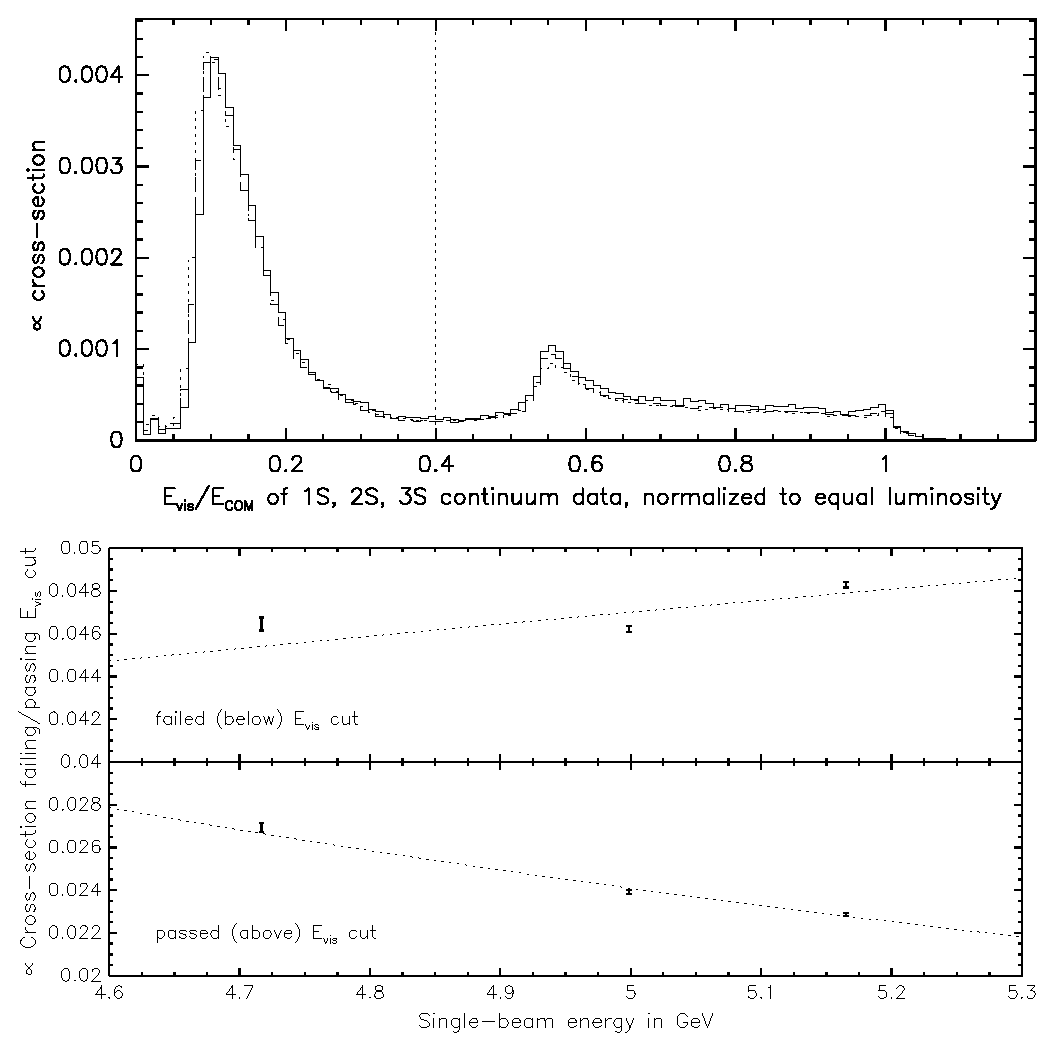
\includegraphics[width=\linewidth]{plots/datasets_twophoton_visen}
  \end{center}
  \caption{\label{datasets:visen_continuum} Top: visible energy from
    unfiltered continuum datasets below $\Upsilon(1S)$,
    $\Upsilon(2S)$, and $\Upsilon(3S)$, with other hadron cuts applied
    except \lfourdec, normalized to equal luminosity using bhabhas.
    Bottom: the integral of the histogram from 0 to 0.4 (``failed
    (below) \visen\ cut'') and from 0.4 to 1.2 (``passed (above)
    \visen\ cut'') versus beam energy.  In each case, $a \log s + b/s$
    has been fit to the points.}
\end{figure}

If I fit the expression
\begin{equation}
  a \log s + b/s \label{datasets:visen_continuum_fitfunc}
\end{equation}
to these three points, I obtain $a/(a+b)$ of 47\% (with an
unbelievable $\chi^2$).  However, if I leave out the first few bins in
\visen, $a/(a+b)$ drops to 17\% (though the three cross-sections still
monotonically increase).  The fit is probably being pulled by unequal
cosmic ray and beam-gas backgrounds in the three continuum datasets.

If I fit the same expression to events that pass the \visen\ cut
(bottom of Figure \ref{datasets:visen_continuum}), $a/(a+b)$ is
0.15\%, negligibly small.  Also, the $\chi^2$ of this fit is 5.8,
which is marginally consistent with one degree of freedom (2\%
confidence level).  From later studies, I know that 1--2\% of the
events that pass the hadron cut can be cosmic rays; inserting
backgrounds on this scale by hand at worst doubles $a/(a+b)$.
Therefore, two-photon backgrounds are negligible after hadron cuts and
the continuum subtraction.

The other backgrounds to be subtracted are beam-gas and cosmic rays.
After the continuum subtraction, it is possible that these backgrounds
have a negative contribution, since the continuum dataset may contain
more beam-gas or cosmic rays than the signal dataset.  Continuing the
technique of subtracting the most heterogeneous control samples first,
the next background to go is beam-gas, because the single-beam
datasets contain cosmic rays.  Here, the scale factors $S_{e^-}$ and
$S_{e^+}$ are the ratios of beam-gas events in the
continuum-subtracted signal to beam-gas events in the single-beam
datasets.  This subtraction is illustrated in Figure
\ref{datasets_beamgas}: beam-gas events are selected in the signal
dataset and in the control dataset, and the control dataset is
normalized to have equal beam-gas.  Note that the beam-gas fraction is
nearly proportional to integrated luminosity, because after the
continuum subtraction, there is little beam-gas left (except for a
little positron-induced beam-gas in the $\Upsilon(2S)$).  This is
another correction whose uncertainty will be taken to be all of
itself.

\begin{figure}[p]
  \begin{center}
    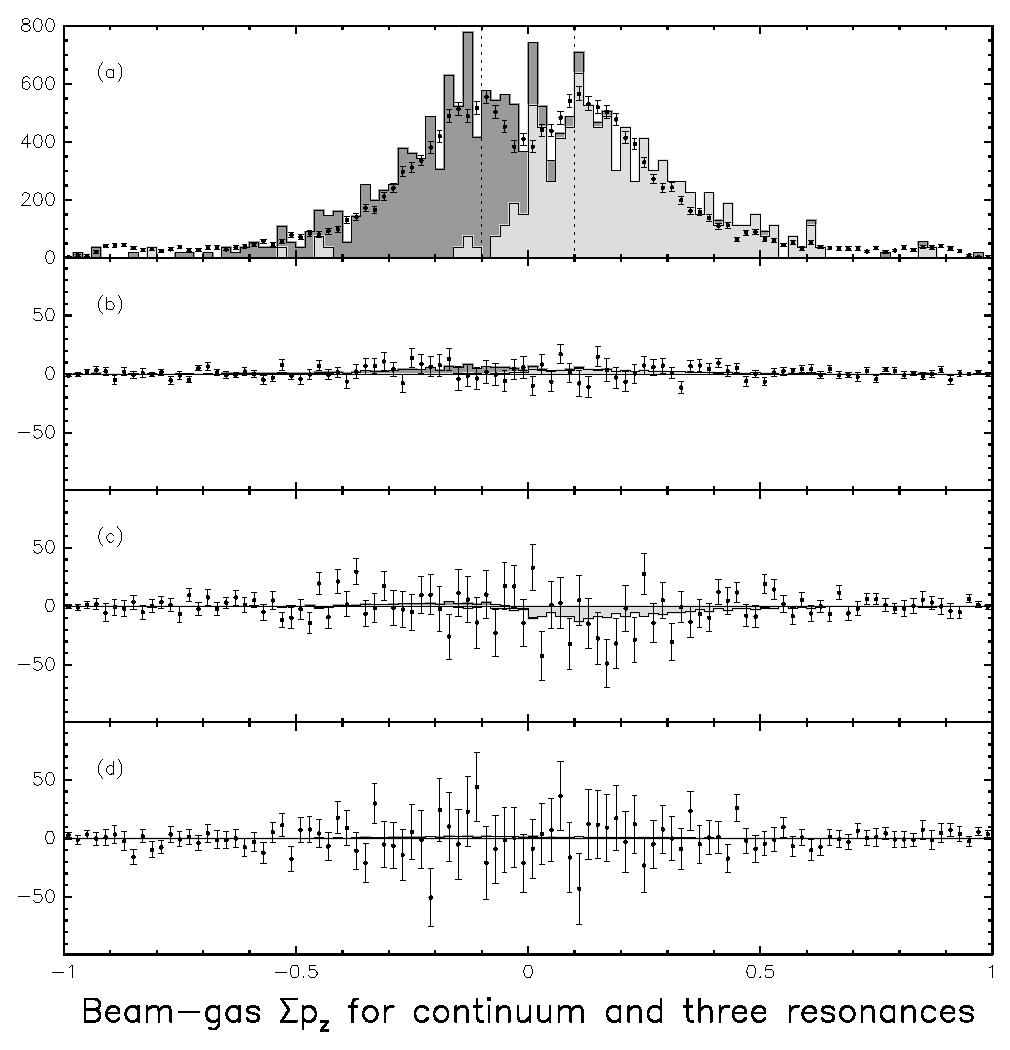
\includegraphics[width=\linewidth]{plots/datasets_beamgas}
  \end{center}
  \caption{\label{datasets_beamgas} Net Z momentum / \ebeam\ from the
    unfiltered dataset, after other beam-gas cuts, in four cases, top
    to bottom: (a) sum of all continuum, (b) continuum-subtracted
    $\Upsilon(1S)$, (c) continuum-subtracted $\Upsilon(2S)$, and (d)
    continuum-subtracted $\Upsilon(3S)$.  The lightly-shaded histogram
    is from positron single-beam and the darker histogram stacked on
    top of it is from electron single-beam.  Dotted lines in
    sub-Figure (a) indicate beam-gas cuts.}
\end{figure}

Finally, cosmic rays are subtracted in the same way.  Cosmic ray cuts
are applied to signal and no-beam control, and $S_0$ is taken to be
their ratio.  This subtraction is illustrated in Figure
\ref{datasets_cosmic}.

Monte Carlo with all $\Upsilon$ decays should look like the unfiltered
data with continuum, beam-gas, and cosmic rays subtracted.

\begin{figure}[p]
  \begin{center}
    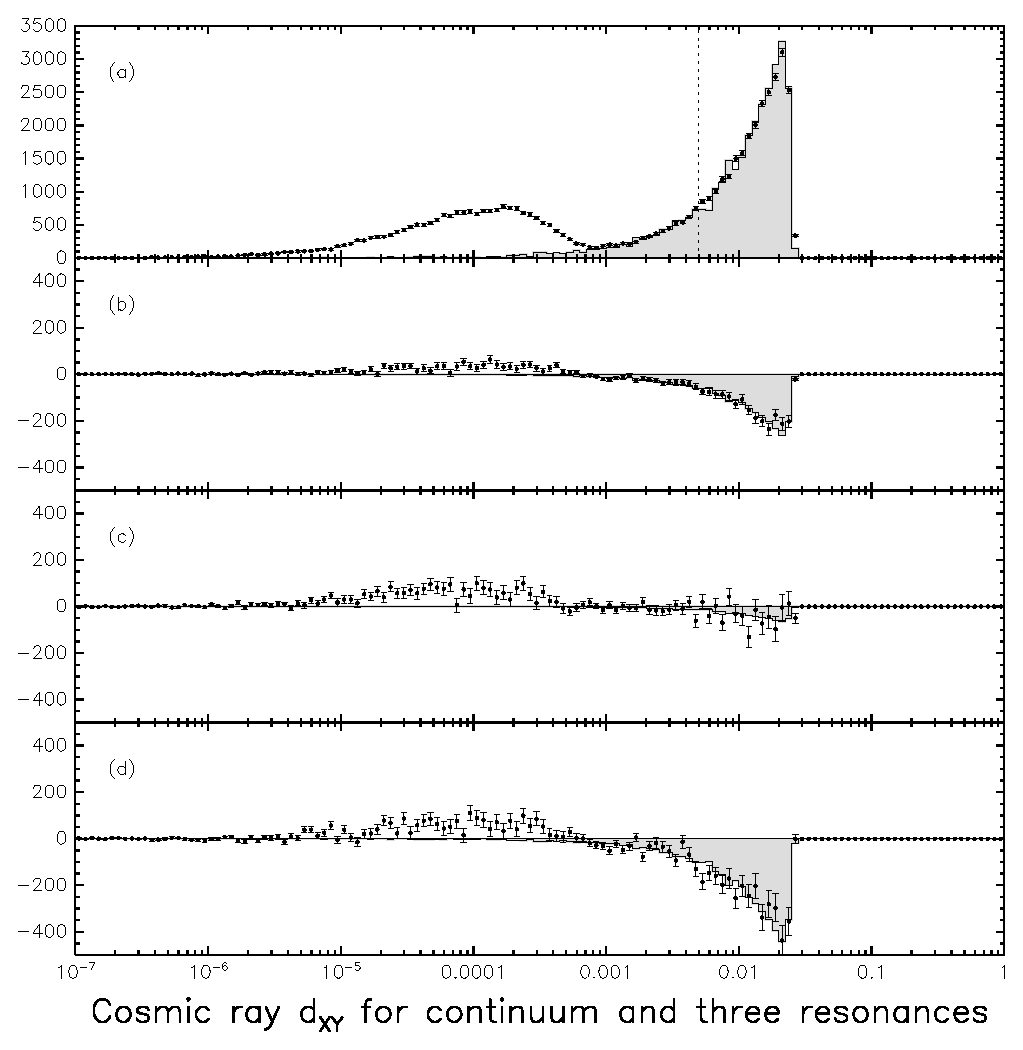
\includegraphics[width=\linewidth]{plots/datasets_cosmic}
  \end{center}
  \caption{\label{datasets_cosmic} Closest track to beam spot XY, in
    log $x$ scale, after other cosmic ray cuts.  The four cases are,
    from top to bottom: (a) sum of all continuum, (b) continuum- and
    beam-gas-subtracted $\Upsilon(1S)$, (c) same for $\Upsilon(2S)$,
    and (d) same for $\Upsilon(3S)$.  The shaded histogram is from the
    no-beam sample, and the dotted line is the cosmic ray cut.  The
    cosmic ray ``peak'' in log $x$ is a flat background in linear $x$.
    The units are meters (so 0.01 is a centimeter, etc.).}
\end{figure}

\section{Scale Factors in the Database Dataset}

The database dataset will be used for lineshape fitting, and I would
rather leave the continuum in the hadron count and fit to it as a
parameter than to subtract it explicitly (and therefore need to
explicitly propagate its uncertainty).  However, beam-gas and cosmic
rays can vary from run to run, so they still must be subtracted
explicitly.

As mentioned above, luminosity will be measured in the database
dataset by counting gamgam events.  Gamgams scale as $1/s$, so the
scale factor for converting hadron counts into something proportional
to hadronic cross section is
\begin{equation}
  S_c^{\mbox{\scriptsize database}} = \mbox{\# gamgams on-res} /
  \mbox{\# gamgams off-res} \times (s_\subs{off-res} /
  s_\subs{on-res})\mbox{.}
\end{equation}
The lineshape fits will be performed after all hadron cuts have been
applied, so the two-photon background is negligible.

As for beam-gas and cosmic rays, we are only interested in how many
survive the hadron cuts.  Passing the no-beam sample through hadron
cuts tells us how many cosmic rays survive (provided that I scale the
no-beam sample to have the same number of cosmic rays as a given run
number), but doing the equivalent thing for beam-gas requires first
removing the cosmic rays from the single-beam samples.  To express
this symbolically,
\begin{flushright}
  \begin{tabular}{r c p{0.7\linewidth}}
    $H_x$, $C_x$, $E_x$, $P_x$ &=& \#events surviving hadron, cosmic
    ray, electron beam-gas, or positron beam-gas, respectively, from
    dataset $x$ \\
  \end{tabular}
  \begin{tabular}{r c p{0.7\linewidth}}
    $x$ &\mbox{ }& can be no-beam, $e^-$-beam, $e^+$-beam, or run, for a
    given run number to be studied \\
  \end{tabular}
  \begin{tabular}{r c p{0.7\linewidth}}
    $N_C$, $N_E$, $N_P$ &=& \#events surviving hadron cuts in
    that run which are really cosmic rays, electron beam-gas, or
    positron beam-gas, respectively.
  \end{tabular}
\end{flushright}
\begin{eqnarray}
  N_C &=& H_\subs{no-beam} \times C_\subs{run} / C_\subs{no-beam}
  \label{datasets_N_C} \\
  N_E &=& (H_\subs{$e^-$-beam} - H_\subs{no-beam} \times
  C_\subs{$e^-$-beam} / C_\subs{no-beam}) \times E_\subs{run} /
  E_\subs{$e^-$-beam} \label{datasets_N_E} \\
  N_P &=& (H_\subs{$e^+$-beam} - H_\subs{no-beam} \times
  C_\subs{$e^+$-beam} / C_\subs{no-beam}) \times P_\subs{run} /
  P_\subs{$e^+$-beam} \label{datasets_N_P}
\end{eqnarray}

The first step in this process (the parenthesized parts of Equations
\ref{datasets_N_E} and \ref{datasets_N_P}) is illustrated in Figure
\ref{datasets:cosmicscale}, where it is also shown that there is very
little feed-through between the beam-gas and cosmic ray cuts.  The
results of these counts, for every run in the database dataset, are
presented in Figure \ref{datasets_databasecontamination}.  For clarity
they are presented as a fraction of the number of continuum
hadrons: if these levels were perfectly flat, there would be no need
to apply any correction, because the backgrounds would be subtracted
along with the continuum.

Beam-gas is a small correction, and it isn't clear how much
non-beam-gas data feeds into the beam-gas cuts (see Figure
\ref{datasets:dxydzcuts}-b).  Therefore, I will apply 50\% $\pm$ 50\%
of the correction.  For a typical run, this means that 0.15\% is
subtracted from the number of hadrons and 0.15\% is added to its
uncertainty.  Cosmic rays are a bigger correction, and the cosmic ray
count represents the number of true cosmic rays to at least 7\% of
itself (see Figure \ref{datasets:dxydzcuts}-a), so the full cosmic ray
correction is applied to each run, propagating only statistical
errors.  Counting statistics from the no-beam sample (which is a 7\%
uncertainty) apply to the whole dataset uniformly, but that can't make
more than a 1\% $\times$ 7\% = 0.07\% difference in the total hadron
count.  I'll just take 0.07\% as a systematic error on $\Gamma_{ee}$.

\begin{figure}[p]
  \begin{center}
    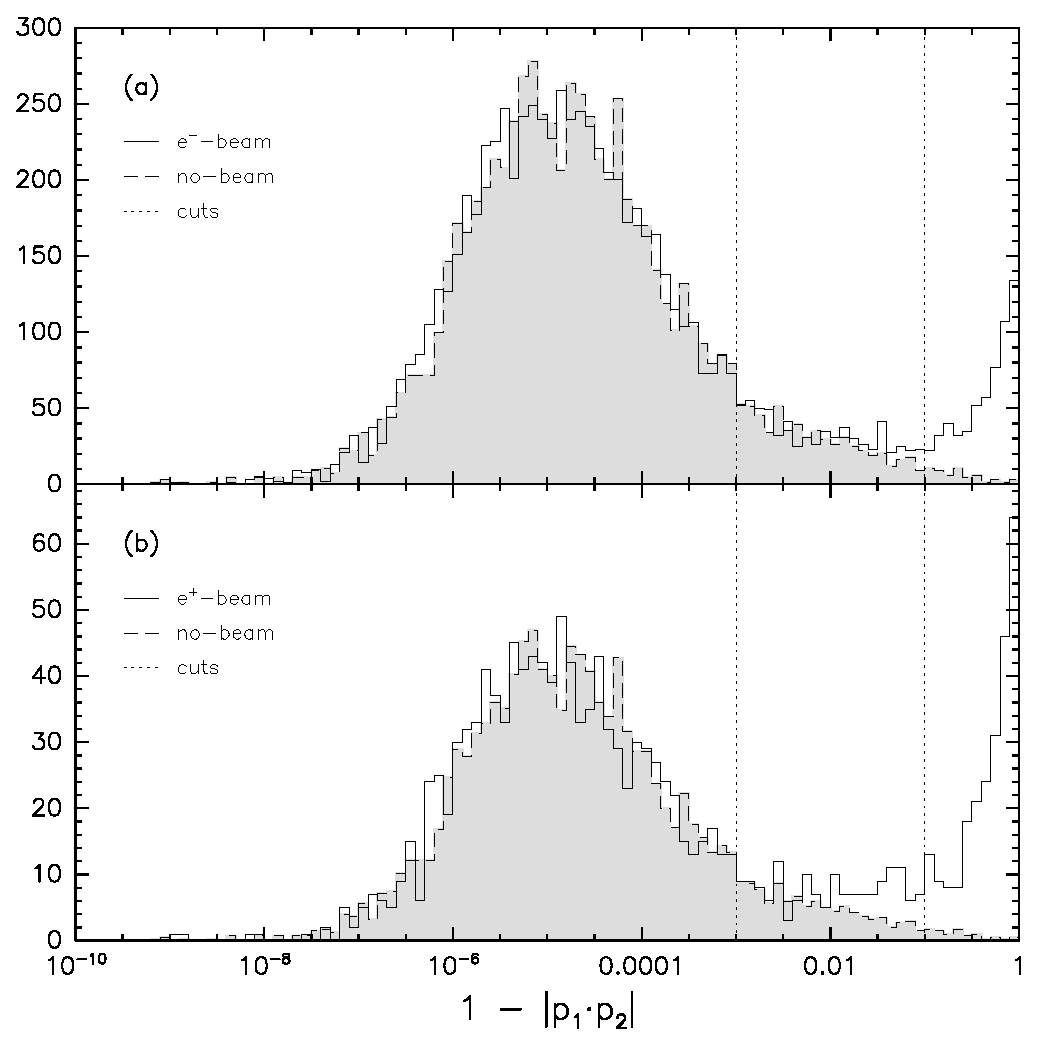
\includegraphics[width=\linewidth]{plots/datasets_cosmicscale}
  \end{center}
  \caption{\label{datasets:cosmicscale} Cosmic-ray back-to-backness
    parameter 1 $-$ \pdotp, in log $x$ scale, after other cosmic ray
    cuts.  Top (a) is electron single-beam and bottom (b) is positron
    single-beam; both are overlaid with the same no-beam sample
    (shaded).  Back-to-back cosmic rays peak around $10^{-5}$, but
    randomly-oriented beam-gas events ``peak'' near 1.  (They are flat
    in linear $x$.)}
\end{figure}

\begin{figure}[p]
  \begin{center}
    \includegraphics[width=\linewidth]{plots/datasets_databasecontamination}
  \end{center}
  \caption{\label{datasets_databasecontamination} Non-beam interaction
    backgrounds that survive hadron cuts ($N_C$, $N_E$, and $N_P$) as
    a percentage of continuum hadrons.  Top to bottom: (a) cosmic
    rays, (b) electron beam-gas, and (c) positron beam-gas.  Dotted
    lines separate $\Upsilon(3S)$, $\Upsilon(1S)$, and $\Upsilon(2S)$
    (from left to right).  Runs used in the unfiltered dataset are
    circled.}
\end{figure}

\begin{figure}[p]
  \begin{center}
    \includegraphics[width=\linewidth]{plots/datasets_database_dxydzcuts}
  \end{center}
  \caption{\label{datasets:dxydzcuts} Geometry cuts which distinguish
    cosmic rays and beam-gas from beam-beam collision data.  Top to
    bottom: (a) closest track to the beam spot in XY for all database
    data (solid histogram) overlaid by no-beam sample (points), with
    other cosmic ray cuts applied, (b) Z of primary vertex for all
    database data (solid histogram) overlaid by a sum of the
    single-beam samples (points), with other beam-gas cuts applied.
    Both are in log $x$ scale with units of meters.}
\end{figure}


%% \chapter{Signal Monte Carlo}
%% \section{Upsilon Monte Carlo}

An implementation of EvtGen was used to simulate $\Upsilon$ decays,
with each of the following generated separately: $\Upsilon \to
e^+e^-$, $\mu^+\mu^-$, $\tau^+\tau^-$, $ggg$, $gg\gamma$, $q\bar{q}$,
and $\Upsilon(2,3S) \to$ all cascade decays.

The three modes with free quarks and gluons are hadronized by JetSet
7.4 before being passed to the detector simulation.  This
hadronization step is an approximation, and that approximation must be
tested.  Another assumption made by the Monte Carlo is that the above
is an exhaustive list of $\Upsilon$ decays (where ``all cascade
decays'' includes only modes listed in the PDG [\ref{cite:pdg}]).  The
study described in the next Chapter will check these assumptions for
$\Upsilon(1S)$, though I will need to assume that cascade decays of
the $\Upsilon(2S)$ and $\Upsilon(3S)$ are well-described by the Monte
Carlo.

The detector simulation and reconstruction were executed using the
same version of code as in the database and unfiltered datasets.  This
is the ``MC code release'' in Table \ref{datasets:unfiltered}
(reconstruction code is guaranteed to be the same as that in the
corresponding ``data code release'').  Where data at one resonance
were processed using two different versions of the code
($\Upsilon(1S)$ and $\Upsilon(2S)$), the same Monte Carlo events were
passed through the different code versions, as a stringent test of
code reproducibility.

This Monte Carlo sample does suffer from one known bug: the
bunch-finding simulation, which is supposed to reproduce CLEO's
identification of which storage ring bunch actually collided to
produce the event, sometimes (rarely) returns too many tested bunches
and an incorrectly identified bunch number.  These failures can be
recognized, and all Monte Carlo tests (except the test for sensitivity
to this bug) rejected bad bunch-finding events.

Extra $\Upsilon$ Monte Carlo was generated for two decay modes.  The
first of these is $\Upsilon(2S) \to \pi^+\pi^- \Upsilon(1S)$, the
``cascade'' decay mode to be studied extensively in the next Chapter.
The other is $\Upsilon(2S,3S) \to \gamma \chi_b(1P,2P) \to \gamma
\gamma \gamma$.  This is a possible background to the gamgam event
type which is sought in Chapter \ref{chp:gamgambkgnds}.  No such
events are seen in real data.

All control files used to generate and process Monte Carlo are listed
in Appendix \ref{chp:appendixmc}.

\section{Gamgam Monte Carlo}

\section{Bhabha Monte Carlo}

Whatever is used for absolute luminosity\ldots




%% \chapter{Upsilons from Di-Pion Cascades}
%% \section{Obtaining an Unbiased Upsilon Sample}

Another way of looking at the $\Upsilon(1S)$ is through the
$\Upsilon(2S) \to \pi^+\pi^- \Upsilon(1S)$ cascade.  The recoil mass
of the two pions has a resolution of 1.5 MeV, so combinatoric
backgrounds can be highly suppressed and the sideband is nearly
linear.  But most importantly, the two pions can be chosen to satisfy
both the trigger and the database event filter, so that the
distribution of $\Upsilon(1S)$ events from the cascades study is
completely unbiased.  All decays of the $\Upsilon(1S)$ will have equal
efficiency, even completely invisible decays to two neutrinos.

One might ask if a similar study can be done for the other resonances:
unfortunately, they cannot.  The $\Upsilon(3S)$ is inaccessible
because the $\Upsilon(4S)$ has a very large decay width to $B\bar{B}$,
which overwhelms any di-pion cascades, and the $\Upsilon(3S) \to
\pi^+\pi^- \Upsilon(2S)$ produces pions with momenta $\le$ 90 MeV, for
which the tracking efficiency is poor.  Also, it isn't worthwhile
adding $\Upsilon(3S) \to \pi^+\pi^- \Upsilon(1S)$ to the
$\Upsilon(1S)$-cascade sample, as this mode adds only 12\% more
events.

There are two differences between $\Upsilon(1S)$ events from the
cascade sample and $\Upsilon(1S)$ events from the database dataset or
unfiltered dataset.  The first is a slight boost due to the recoil of
the two pions, but the maximum $\beta$ and $\gamma$ for the
$\Upsilon(1S)$ is 0.058 and 1.0033, respectively.  Another is the
possibility of track confusion with the pions.  An $\Upsilon(1S)$
track might overlap one of the pion tracks and go undiscovered, or two
tracks could be fitted to one pion, where one of them is identified as
the pion and the other is assumed to belong to the $\Upsilon(1S)$.
Both of these effects would be captured in a Monte Carlo simulation,
so $\Upsilon(2S) \to \pi^+\pi^- \Upsilon(1S)$ Monte Carlo is passed
through the same analysis as data.  Measurements from cascade Monte
Carlo can be compared with measurements from direct $\Upsilon(1S)$
Monte Carlo, and this can be used to determine a translation factor.

After two tracks in the event have been identified as belonging to the
cascade pions, they are excluded from the calculation of all cut
variables, \dxy, \dz, \pone, and \visen, and I directly measure the
cut efficiency by asking how many $\Upsilon(1S)$ events pass and how
many fail.  Ideally, I would exclude pions from the trigger as well,
but the low-level trigger variables are not available in the database
dataset.  Instead, I will bound the trigger efficiency by measuring a
looser cut and a tighter cut.

\subsection{Constraints on the Two Pion Tracks}

As a reminder, the following is a set of sufficient conditions for an
event to appear in the database dataset (see page
\pageref{wonderfuldiscovery}):
\begin{enumerate}
  \item the event passes a hardware trigger,
  \item it has two or more quality tracks,
  \item it has \hotvisen\ $>$ 4\% \ecom, and
  \item it passes \lfourdec.
\end{enumerate}
I need to choose pion tracks such that the above criteria are
satisfied by the pions alone, leaving the $\Upsilon(1S)$ free to decay
however it likes.

The first criterion can be satisfied by requesting only events which
pass the TwoTrack trigger, and then making sure that my pions alone
generate the two AXIAL tracks needed to satisfy that trigger line.  An
independent study of trigger tracking efficiency [\ref{cite:inga}]
found that if a track is reconstructed in software and has a
transverse momentum ($p_T$) $>$ 150 MeV, an AXIAL track is found at
the same $\phi$ ($\pm$ 5$^\circ$) with 99.93 $\pm$ 0.07\% efficiency.
Therefore, I will require all of my pions to have $p_T$ $>$ 150 MeV.

I am also interested in $\Upsilon(1S)$ events that pass some trigger
requirements.  After the pions guarantee two AXIAL tracks, the Hadron
trigger line only requires 1 additional AXIAL track and 1 CBLO.  All
the trigger lines that I am interested in require at least 1 AXIAL
track and 1 CBLO from the $\Upsilon$, so I acquire another sample of
di-pion cascades that passes the Hadron trigger, with the same
restrictions on pion tracks.  This way, some of my measurements can
evade the TwoTrack prescale.

I will call these two cascades samples ``little'' (from the TwoTrack
trigger line) and ``big'' (from the Hadron trigger line).  The little
sample is completely unbiased, and the big sample is biased in a way
that partly simulates the trigger.

Criteria \#2 and \#3 can be satisfied by requiring the two pions to be
quality tracks.  The energy of all quality tracks (assuming each to
have the mass of a charged pion) is included in \visen, and the
kinematics of the decay gives the two recoil pions 563 MeV.  The 4\%
threshold is 401 MeV, so this is always automatically satisfied.

A sufficient condition for \lfourdec\ is to require two tracks with
the following cuts (on quantities saved after pattern recognition but
before track fitting).  I require the two pion tracks to satisfy them.
\begin{itemize}
  \item The track must have some Z information (meaning that it
    reached the stereo layers of the DR, which is equivalent to the
    $p_t$ cut),

  \item it must have more than 40\% of its expected number of hits,

  \item $|\cos\theta|$ $<$ 0.93,

  \item $\chi^2$ $<$ 20 $\times$ the number of degrees of freedom, and

  \item it must approach the DR origin within 2.5 cm in XY and 15 cm
    in Z.
\end{itemize}

\subsection{Excluding Cascade Pion Curlers}

There is one last consideration to make before measuring cut
efficiencies: while the tracks identified as pions have been excluded
from the calculation of all $\Upsilon(1S)$ variables, a pion might
complete a full orbit around its gyration circumference and yet remain
in the detector to be measured again.  Such circular loops are
identified by the track recognition software as two (or more) tracks,
known as ``curlers.''  Because of the vertexing requirements I placed
on the pions, I always identify the track associated with the first
half-orbit.

Curlers can be eliminated from the cascades sample by cutting on the
pions' $p_z$.  The arclength (in XY projection) of an orbit is given
by
\begin{equation}
  2\pi \, \frac{p_T}{3\times 10^{-4} \, \cdot \, 1.4 \mbox{T}} \,
  \frac{\mbox{T cm}}{\mbox{MeV}}
\end{equation}
and the speed of the particle (in XY projection, $c=1$) by
\begin{equation}
  \frac{p_T}{\sqrt{{m_\pi}^2 + |\vec{p}|^2}}
\end{equation}
so the time to complete a half-orbit is
\begin{equation}
  \frac{2\pi}{4.2} \, \sqrt{{m_\pi}^2 + |\vec{p}|^2} \,
  \frac{\mbox{cm}}{\mbox{MeV}}\mbox{ (in units of cm).}
\end{equation}
Similarly, the time for the particle to move a distance $L$ in the Z
direction is
\begin{equation}
  \frac{\sqrt{{m_\pi}^2 + |\vec{p}|^2}}{p_z} \, L
\end{equation}
so the particle completes a half-orbit as it translates a distance $L$
in the Z direction if its momentum Z-component is
\begin{equation}
  \frac{2.1}{\pi} \, L \, \frac{\mbox{MeV}}{\mbox{cm}} \mbox{.}
\end{equation}
The axial section of the DR is 90 cm long in Z: this corresponds to a
$|p_z|$ of 60 MeV.  I will only accept cascade pions with a $p_z$
outside of this range.

\subsection{Recoil Mass Peak and Sideband Subtraction}

Now that I have chosen pairs of tracks which guarantee inclusion in my
sample, I use the following algorithm to reconstruct a recoil mass
peak:
\begin{enumerate}
  \item Calculate
    \begin{equation}
      m_{\pi\pi \mbox{\scriptsize -rec}} = \sqrt{(2
        E_\subs{beam} - \sqrt{|\vec{p}_1|^2 + {m_\pi}^2} -
	  \sqrt{|\vec{p}_2|^2 + {m_\pi}^2})^2 - |\vec{p}_1 +
	      \vec{p}_2|^2}
    \end{equation}
  for each pair of good tracks with momenta $\vec{p}_1$ and
  $\vec{p}_2$ at their intersection point in XY.  Each pair of tracks
  must also have opposite charges.

  \item From the set of all $m_{\pi\pi \mbox{\scriptsize -rec}}$
  combinations that are within 20 MeV of the $\Upsilon(1S)$ mass,
  intersect each other within 5 mm of the beamspot in XY and 5 cm in
  average Z (with a 2.5 cm tolerance for missing each other in Z),
  I randomly choose one.  If the set is empty, I skip the event.
\end{enumerate}

The random choice is introduced in step \#2 to make sure that the
combinatoric background doesn't peak under the signal.  Figure
\ref{cascades_recoilmass} is a plot of the recoil mass, showing the
9.454--9.472 GeV signal region and the 9.441--9.480 GeV sideband.
(The sideband includes events from both sides of the peak, excluding
the signal region.)

\begin{figure}[p]
  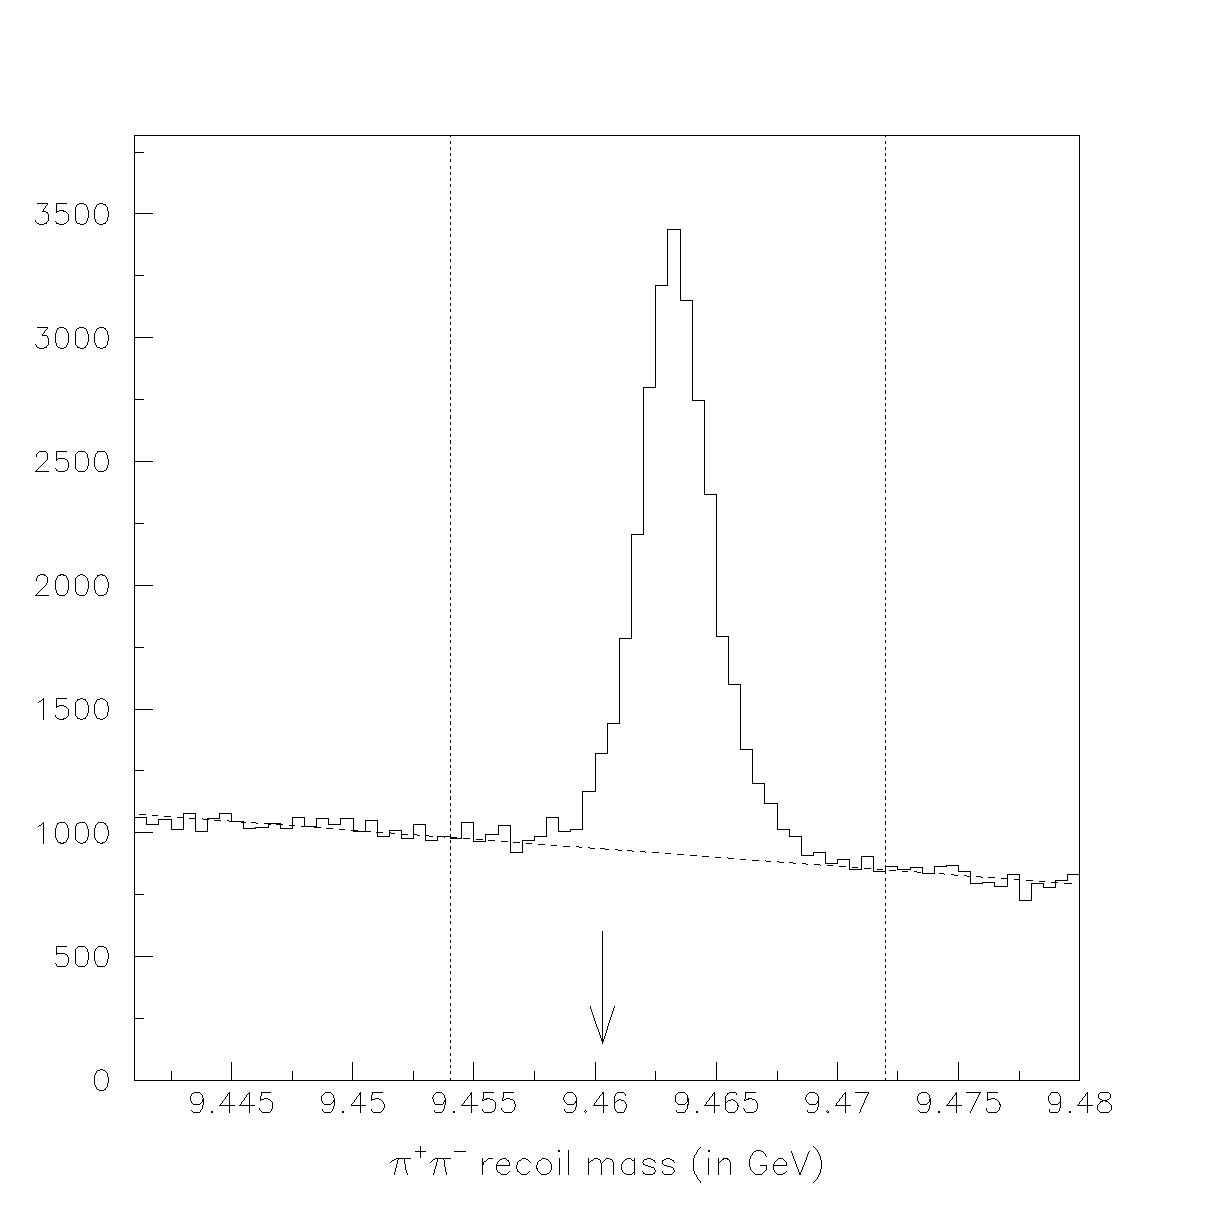
\includegraphics[width=\linewidth]{plots/cascades_recoilmass}
  \caption{\label{cascades_recoilmass} Recoil mass of the two pions in
  $\Upsilon(2S) \to \pi^+\pi^- \Upsilon(1S)$, from the TwoTrack
  trigger line (top) and from the Hadron trigger line (bottom).
  Dotted lines separate signal from sideband, and the dashed lines are
  quadratic fits to the sideband.  The arrows point to the true mass
  of the $\Upsilon(1S)$.}
\end{figure}

The combinatoric background in Figure \ref{cascades_recoilmass} is a
smooth distribution whose characteristic width is much greater than
the 39 MeV-wide plot window.  It can therefore be expanded as a
polynomial.  The distribution looks linear, but I want to bound the
error I incur from truncating the polynomial.  To do this, I use the
following fit function:
\begin{multline}
  f(m; c_0, c_1, c_2) = c_0(1) + c_1 (m - 9.458357142857055) + \\
  + c_2 (m^2-18.92233477371051 m+89.51347812358851) \label{cascades:eqn_fitfunc}
\end{multline}
where $m$ is the di-pion recoil mass, $c_0$, $c_1$, and $c_2$ are the
fit parameters.  (Yes, all of those digits are necessary!)  The three
parenthesized polynomials were chosen to be orthogonal to each other
in the sideband region, so that the fit parameters are uncorrelated
and can be individually varied for a systematic error.

I use the best-fit of the sideband to Equation
\ref{cascades:eqn_fitfunc} to interpolate under the peak, and
integrate for the number of events in the sideband and the number of
combinatoric background events in the signal region.  The ratio of
these tells me how to subtract sideband from signal, which I do to
produce plots of every variable that defines the hadron event type.
Cut efficiencies are read off the plots, and errors in $c_0$, $c_1$,
and $c_2$ are propagated into those efficiencies.  In every fit, the
quadratic term is consistent with being zero, as the background
distribution is nearly linear.  This uncertainty in $c_2$ is the
truncation error I wanted to determine.

\section{Minimal and Maximal Triggers}

With an unbiased sample of $\Upsilon(1S)$ events, I can find the
efficiency of any cut independently of all the others.  That is,
except for the trigger: the number of AXIAL tracks is not available in
the database dataset, so I cannot subtract two and recalculate the
trigger decision.  Unfortunately, I do need to know the trigger
efficiency independently of all other cuts, and I need to know the
efficiency of all other cuts with the trigger applied.  Therefore, I
must construct something like the trigger out of information which is
available to me.  (Here, the trigger in question is ``Hadron or RadTau
or ElTrack.'')

I construct two such things: what I call the ``minimal trigger,'' which
is a necessary condition for the trigger to pass an event, and the
``maximal trigger,'' which is a sufficient condition.  The efficiency
of the minimal trigger will be greater than the efficiency of the true
trigger, and the efficiency of the maximal trigger will be less than
the efficiency of the true trigger.  (The true trigger efficiency is
close to 100\%, so I will only really need the maximal trigger for
trigger efficiency measurements.  But for measurements with the
trigger applied, I will need both.)

After the two pions generate two AXIAL tracks, the Hadron trigger line
additionally requires 1 AXIAL track and 1 CBLO from the $\Upsilon(1S)$
event (as mentioned above).  The true trigger requires more than this
from a direct $\Upsilon(1S)$ event ($e^+e^- \to \Upsilon(1S)$), so the
Hadron trigger line is a minimal trigger for cascade $\Upsilon(1S)$
events.  (It is possible that one of the cascade pions is somehow
responsible for the third AXIAL track or the CBLO, but that only makes
the minimal trigger more minimal.)  When the minimal trigger is
applied, I am free to use the ``big'' cascades sample for more
statistical power.

Since I know that any reconstructed track with $p_T$ $>$ 150 MeV (call
it a high-$p_T$ track) generates an AXIAL track with high probability,
the number of high-$p_T$ tracks is less than or equal to the number of
AXIAL tracks.  I can construct a cut which is tighter than the trigger
(the ``maximal trigger'') like this:
\begin{center}
  (\#high-$p_T$ tracks $\ge$ 3 and \#CBLO $\ge$ 1) or \mbox{\hspace{6 cm}} \\
  (\#STEREO tracks $\ge$ 2 and (\#CBLO $\ge$ 2 or \#CBMD $\ge$ 1)) or \\
  \mbox{\hspace{5 cm}} (\#high-$p_T$ tracks $\ge$ 1 and \#CBMD $\ge$ 1).
\end{center}
I can satisfy \#CBLO $\ge$ 1 by requesting the Hadron trigger line,
and \#CBMD $\ge$ 1 by requesting the ElTrack trigger line, as long as
the two pions did not contribute any energy to the CC.  This can be
guaranteed by forcing both pions to have $p_T$ $<$ 200 MeV, so that
their gyration orbits are 5 cm too small to reach the CC.  This
additional constraint can change the shape of the combinatoric
background distribution, so I need a different fit when I use the
maximal trigger.  Since the maximal trigger includes the minimal
trigger, I can use the ``big'' cascades sample.

The second line of the maximal trigger is exactly the same as RadTau,
and it can be obtained by asking for the RadTau trigger line itself
because the two pions do not satisfy it.  The proof of this comes from
looking at events that satisfy TwoTrack and ElTrack but not Hadron.
ElTrack gives the event a CBMD, which satisfies the neutral part of
RadTau, and refusing the Hadron trigger line limits the event to only
two AXIAL tracks, so any STEREO tracks must be extensions of the AXIAL
tracks the pions generated.  There are 39 such events in my cascade
sample (almost certainly all combinatoric background, not real cascade
decays).  Of these, 8 satisfy RadTau, but all 8 have large $p_T$,
while I am restricting my two pions to have small $p_T$.  The
distribution of $p_{T1} + p_{T2}$ for RadTau-satisfying events has a
mean of 482 MeV and a standard deviation of 5 MeV (they are all at the
extreme limit of the kinematically-allowed range), while I only accept
events with $p_{T1} + p_{T2}$ $<$ 400 MeV in the maximal trigger.
(This is the extra constraint I imposed at the end of the previous
paragraph.)  This is 16 standard deviations away.  Therefore, pions
chosen for the maximal trigger never generate STEREO tracks, and any
STEREO tracks in the event must have come from the $\Upsilon(1S)$.

\section{Results: Plots and Cut Efficiencies}

All combinatoric background fits successfully converged with accurate
error matrices, parabolic errors close to their fully non-linear
errors, correlations between the parameters less than 20\%, and
$\chi^2$ confidence levels between 10\% and 96\%.

The distributions of \dxy, \dz, \pone, \visen, and the number of
quality tracks are shown in Figures \ref{cascades_logd0close},
\ref{cascades_logwz}, \ref{cascades_p1}, \ref{cascades_visen}, and
\ref{cascades_tracks}.

\begin{figure}[p]
  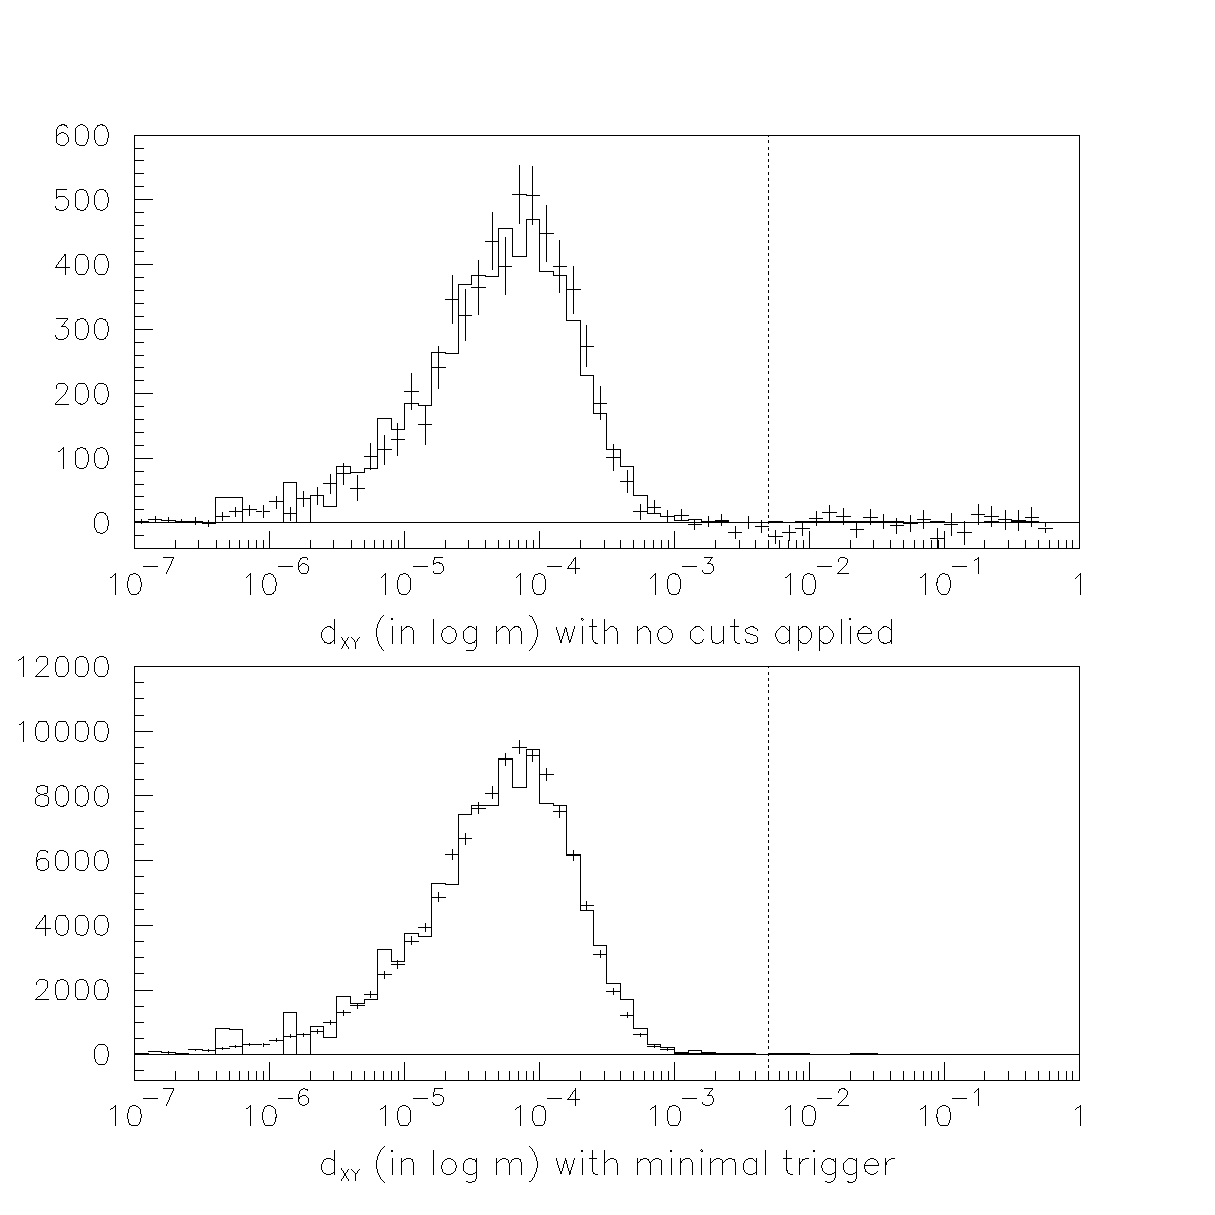
\includegraphics[width=\linewidth]{plots/cascades_logd0close}
  \caption{\label{cascades_logd0close} Closest track to beam spot XY
  in log $x$ scale ($\pi^+\pi^-$ removed, sideband-subtracted),
  without any cuts (top) and after requiring the minimal trigger
  (bottom).  The dotted line is the cut boundary, and the solid
  histogram is Monte Carlo.}
\end{figure}

\begin{figure}[p]
  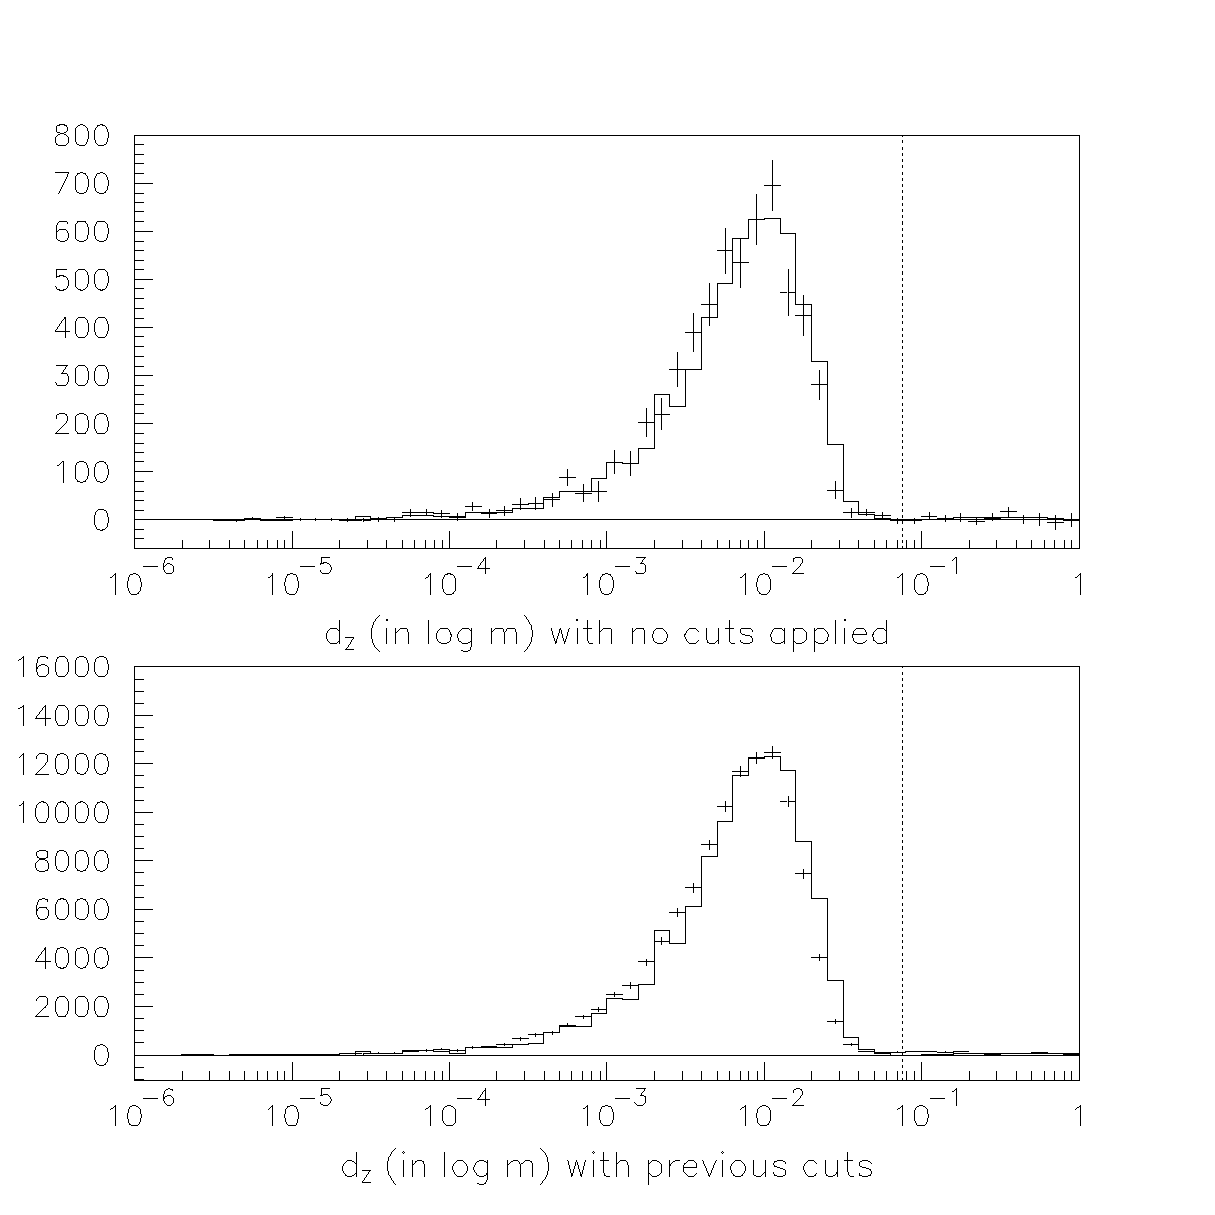
\includegraphics[width=\linewidth]{plots/cascades_logwz}
  \caption{\label{cascades_logwz} Z of primary vertex in log $x$ scale
  ($\pi^+\pi^-$ removed, sideband-subtracted), without any cuts (top)
  and after requiring previous cuts (bottom).  The dotted line is the
  cut boundary, and the solid histogram is Monte Carlo.}
\end{figure}

\begin{figure}[p]
  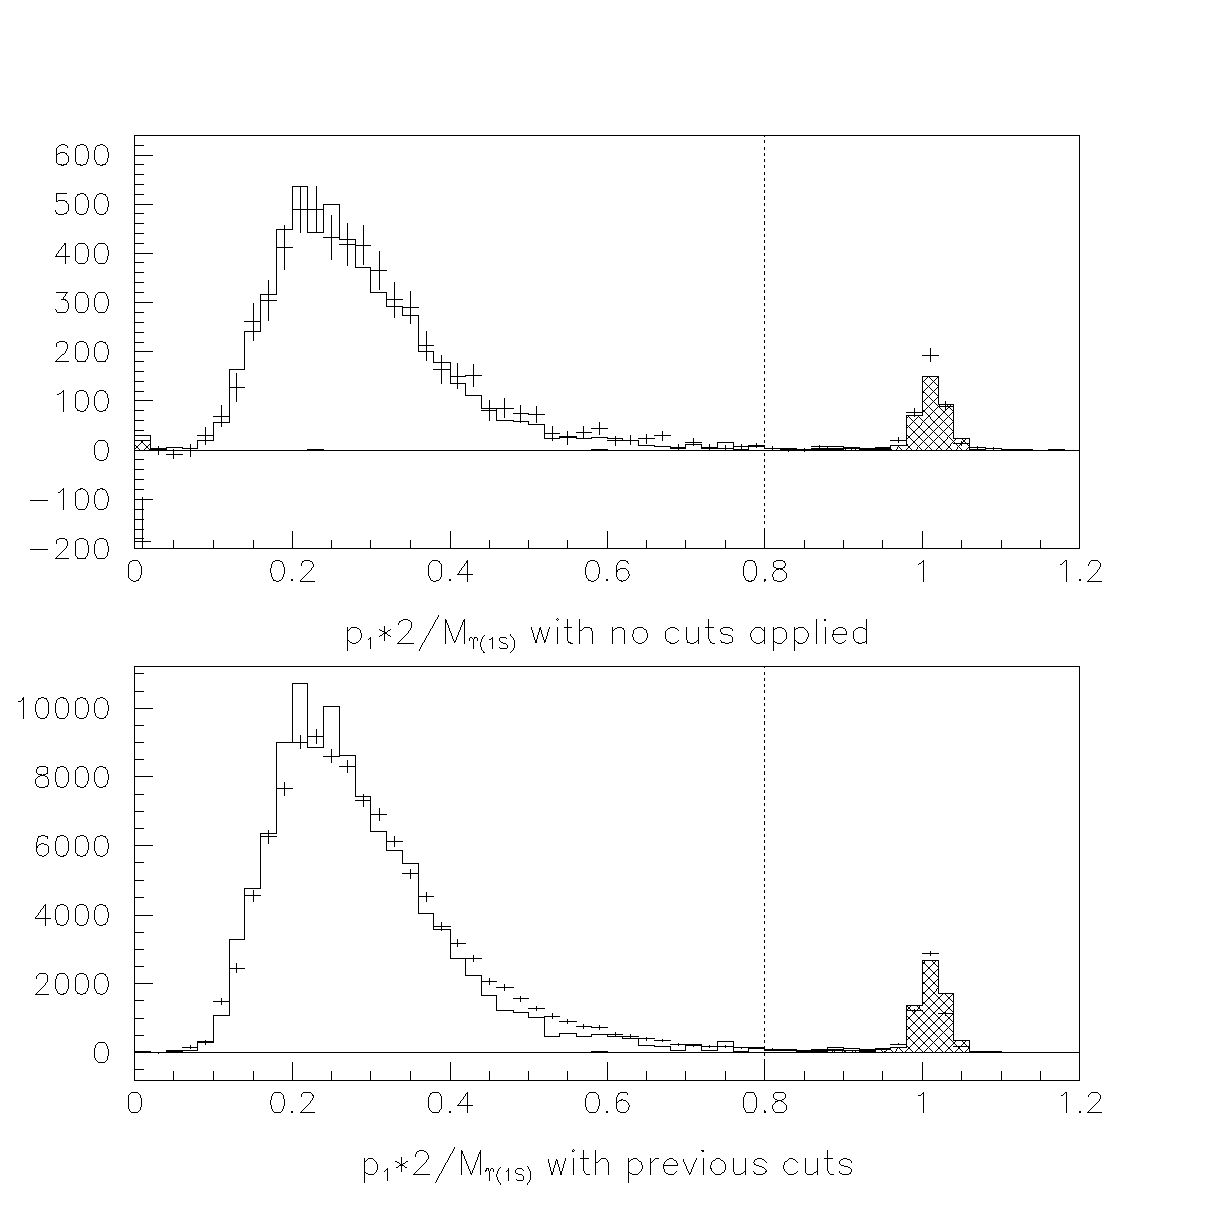
\includegraphics[width=\linewidth]{plots/cascades_p1}
  \caption{\label{cascades_p1} Momentum of biggest track divided by
  $M_{\Upsilon(1S)}/2$ ($\pi^+\pi^-$ removed, sideband-subtracted),
  without any cuts (top) and after requiring previous cuts (bottom).
  The dotted line is the cut boundary, and the solid histogram is
  Monte Carlo.  The cross-hatched histogram is Monte Carlo
  $\Upsilon(1S) \to e^+e^-$ and $\mu^+\mu^-$.}
\end{figure}

\begin{figure}[p]
  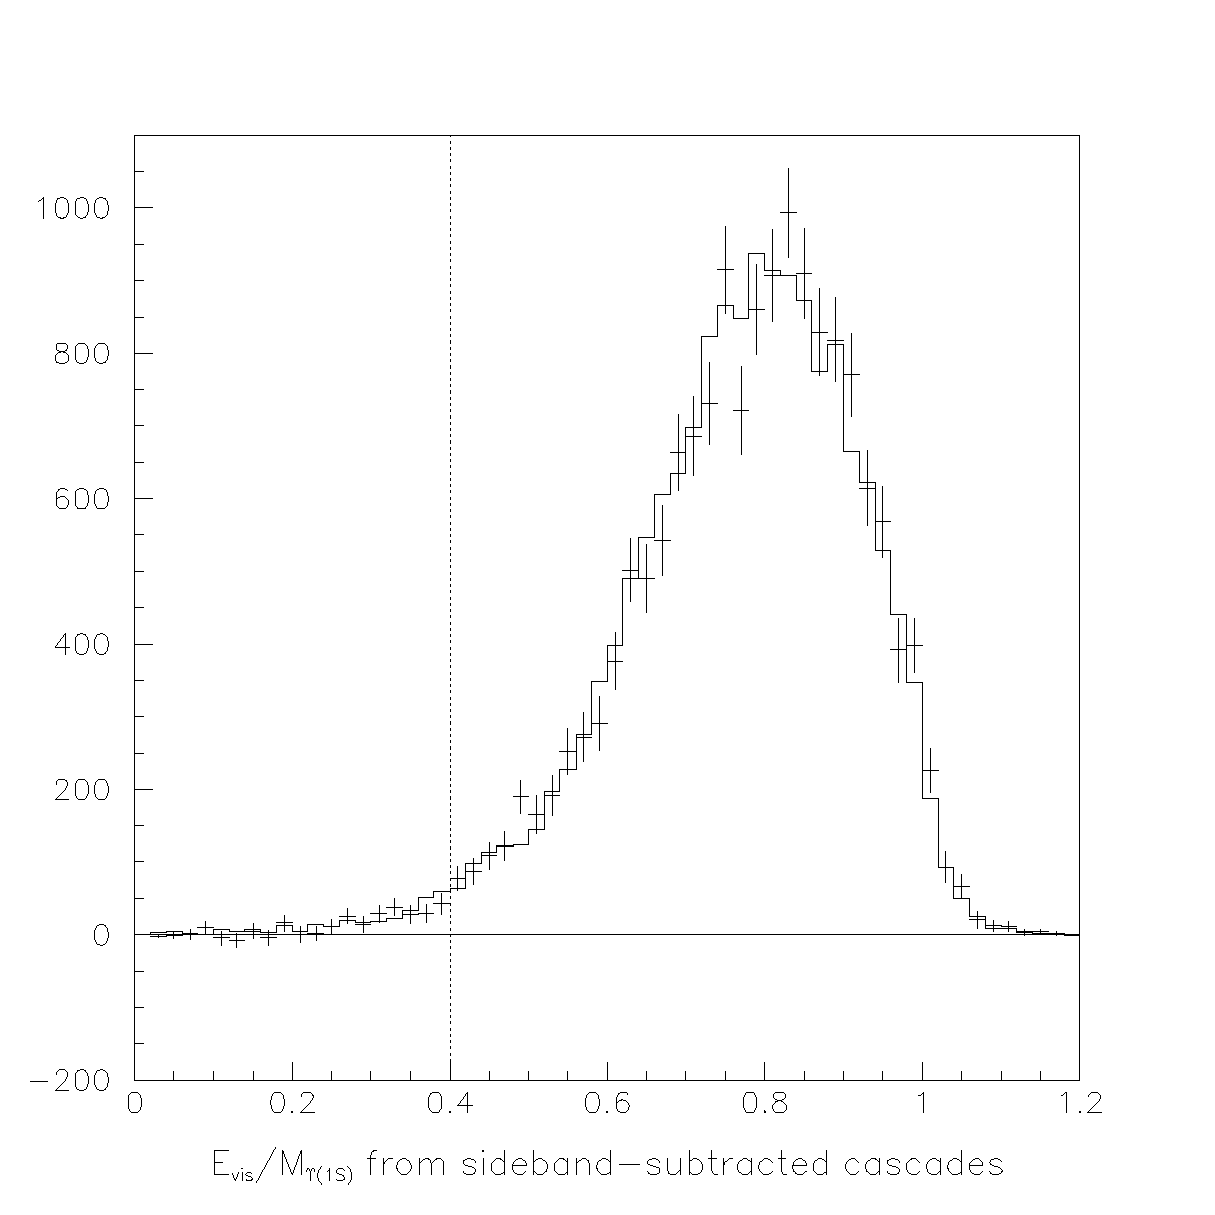
\includegraphics[width=\linewidth]{plots/cascades_visen}
  \caption{\label{cascades_visen} Visible energy divided by
  $M_{\Upsilon(1S)}$ ($\pi^+\pi^-$ removed, sideband-subtracted),
  without any cuts (top) and after requiring previous cuts (bottom).
  The dotted line is the cut boundary, and the solid histogram is
  Monte Carlo.}
\end{figure}

\begin{figure}[p]
  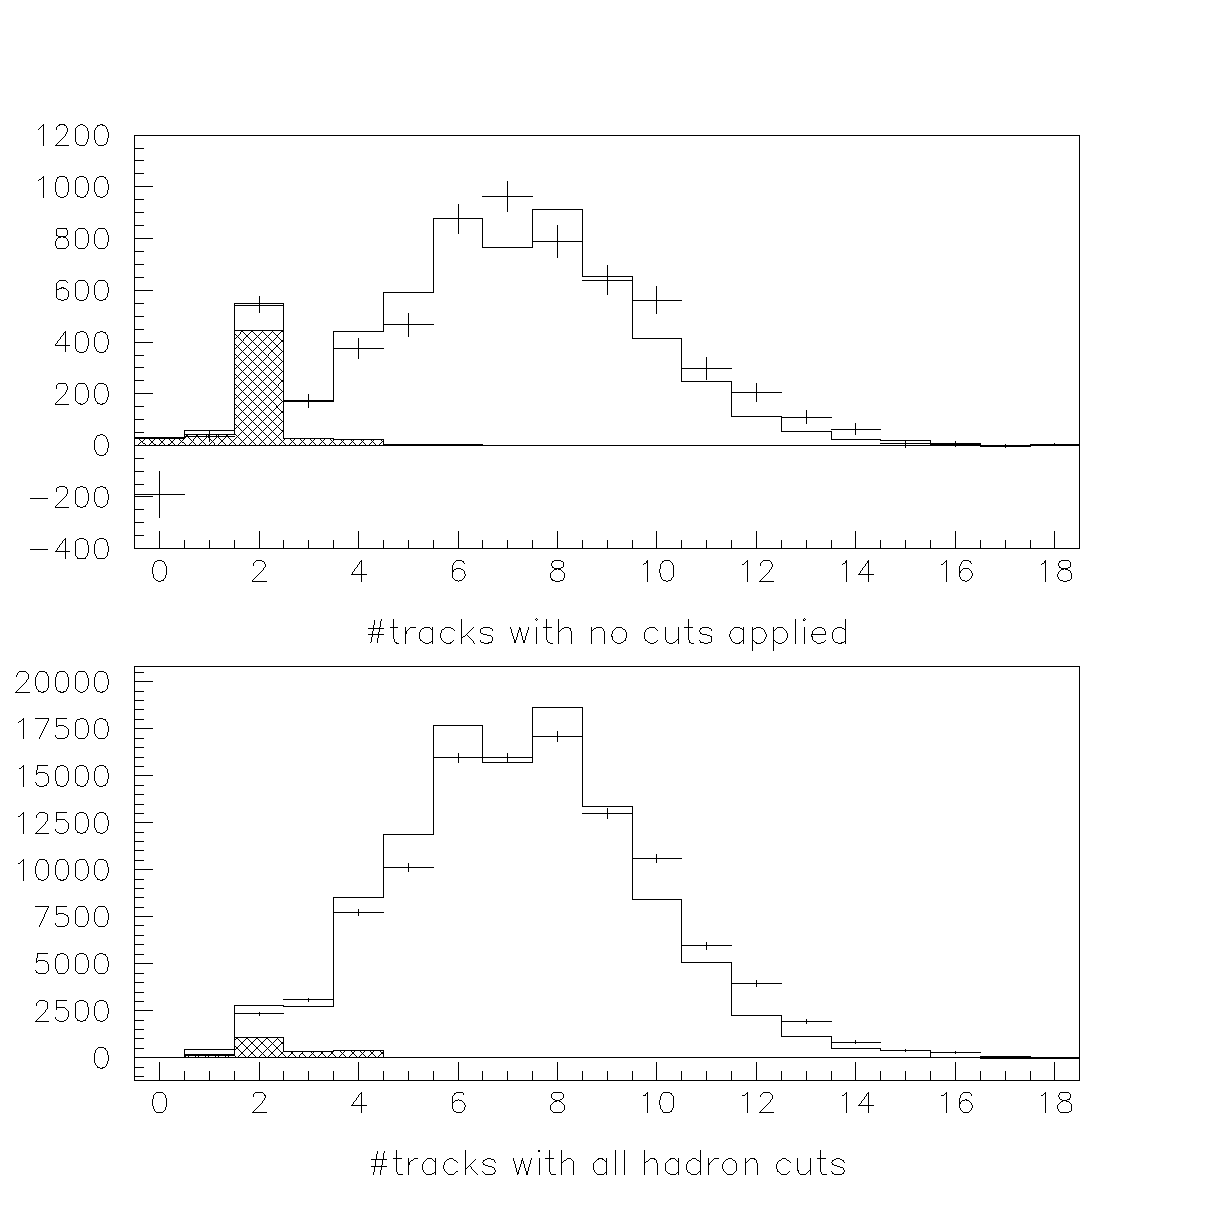
\includegraphics[width=\linewidth]{plots/cascades_tracks}
  \caption{\label{cascades_tracks} Number of quality tracks
  ($\pi^+\pi^-$ removed, sideband-subtracted), without any cuts (top)
  and after requiring all hadron cuts (bottom).  The solid histogram
  is Monte Carlo, and the cross-hatched histogram is Monte Carlo
  $\Upsilon(1S) \to e^+e^-$, $\mu^+\mu^-$, and $\tau^+\tau^-$ (in
  the bottom plot, almost entirely $\tau^+\tau^-$).}
\end{figure}

In Table \ref{cascades_table}, cut efficiencies have been calculated
by counting events with the cut applied ($A$), counting events with
the negation of the cut applied ($B$) and reporting
\begin{equation}
  \frac{A}{A+B} \pm \frac{\sqrt{{\sigma_A}^2 B^2 + {\sigma_B}^2
  A^2}}{(A+B)^2} \mbox{.}
\end{equation}
These statistical uncertainties have been added in quadrature with
sideband fit uncertainties (which were usually smaller than 0.05\%).
Cumulative cuts either have the minimal trigger applied or the maximal
trigger applied; the value I quote is the average of the two with half
the difference added in quadrature to the error.  (This correction is
also usually smaller than the statistical uncertainties.)

The minimal trigger efficiency in data is 102.5 $\pm$ 1.9\%; it has
statistically fluctuated above the maximum allowed value of 100\%.
(The sideband subtraction made this possible.)  The probability
distribution for the trigger efficiency is
\begin{equation}
  P(\varepsilon) = \exp(-(\varepsilon - 102.5)^2/2/1.9^2) / \sqrt{2 \pi} / 1.9 \mbox{,}
\end{equation}
so if I impose the constraint that the efficiency cannot be above
100\%, only the tail below 100\% remains (9.4\% of the a priori
probability).  This distribution has a mean and standard deviation of
99.11 $\pm$ 0.77\%.  This is what I will quote as the value and error
of the minimal trigger efficiency in data, though I'm sufficiently
uncomfortable about it that I devote the next Chapter to measuring the
trigger efficiency by other means.

The maximal trigger efficiency {\it given} the minimal trigger is very
well known in data (99.55 $\pm$ 0.12\%) because some of the background
is suppressed and this measurement comes from a data sample which is
not prescaled.  Therefore I compute the total efficiency of the
maximal trigger by applying
\begin{equation}
  P(\mbox{maximal trigger}) = P(\mbox{maximal trigger} | \mbox{minimal
  trigger}) \times P(\mbox{minimal trigger})\mbox{.}
\end{equation}
The Monte Carlo has much smaller backgrounds, so its maximal trigger
efficiency can be measured directly.

The most precise measurements of cut efficiency are cumulative, the
efficiency of each cut with all previous cuts applied.  These have
been listed between the two horizontal lines in Table
\ref{cascades_table}.  The total efficiency is just the product of
these times the trigger efficiency, though I can avoid
multiply-counting errors by measuring the efficiency of all cuts
except the trigger as a single cut.  This is presented below the
second line in the Table.  For the efficiency of all cuts, I must
multiply by the trigger efficiency, which is assumed to be the average
of the minimal and maximal trigger efficiencies with half the
difference as error.  (In data, the minimal and maximal trigger
efficiencies have almost entirely correlated errors, so this error is
counted only once.)

\begin{table}
  \caption{\label{cascades_table} Efficiency of each cut in cascade
  data, cascade Monte Carlo, and direct $e^+e^- \to \Upsilon(1S)$
  Monte Carlo.  Each line includes all decay modes except when
  otherwise noted.  Direct Monte Carlo errors are in the last digit
  presented.}
  \begin{center}
    \begin{tabular}{p{0.4\linewidth} c c c}
      & data & Monte Carlo & direct $\Upsilon$ \\\hline
      minimal trigger                	     & 99.11 $\pm$ 0.77\%   & 98.77 $\pm$ 0.17\% & \\
      maximal trigger                	     & 98.66 $\pm$ 0.78\%   & 97.77 $\pm$ 0.54\% & \\
      true trigger                   	     &                      &                    & 98.50\% \\\hline
      \dxy\ $<$ 5 mm given trigger   	     & 99.951 $\pm$ 0.031\% & 99.89 $\pm$ 0.13\% & 99.97\% \\
      \dz\ $<$ 7.5 cm given previous 	     & 99.23 $\pm$ 0.15\%   & 99.64 $\pm$ 0.21\% & 99.81\% \\
      \pone\ $<$ 80\% \ebeam\ given previous & 94.68 $\pm$ 0.21\%   & 93.48 $\pm$ 1.0\%  & 95.04\% \\
      \pone\ (hadronic decays)               & 99.72 $\pm$ 0.27\%   & 99.80 $\pm$ 0.21\% & 99.87\% \\
      \visen\ $>$ 40\% \ecom\ given previous & 98.90 $\pm$ 0.28\%   & 98.05 $\pm$ 0.62\% & 98.78\% \\\hline
      everything given trigger               & 92.87 $\pm$ 0.42\%   & 91.2 $\pm$ 1.3\%   & \\
      assumed trigger efficiency             & 98.89 $\pm$ 0.78\%   & 98.27 $\pm$ 0.56\% & \\
      everything                             & 91.84 $\pm$ 0.84\%   & 89.6 $\pm$ 1.3\%   & 93.89\% \\
      everything (hadronic decays)           & 97.68 $\pm$ 0.92\%   & 98.37 $\pm$ 0.61\% & 98.72\% \\
    \end{tabular}
  \end{center}
\end{table}

For two cuts (``\pone\ $<$ 80\% \ebeam'' and ``everything''), I want
to calculate the efficiency of only hadronic decay modes: all modes
except $\Upsilon(1S) \to e^+e^-$, $\mu^+\mu^-$, and $\tau^+\tau^-$.
For this I rely on previous measurements of the $\Upsilon(1S)$
branching fractions and the Monte Carlo's simulation of the leptonic
decays.  Without assuming lepton universality, these branching
fractions are
\begin{eqnarray}
  \mathcal{B}_{ee} &=& 2.38 \pm 0.11\% [\ref{cite:pdg}] \\
  \mathcal{B}_{\mu\mu} &=& 2.49 \pm 0.07\% [\ref{cite:istvan}] \\
  \mathcal{B}_{\tau\tau} &=& 2.67 \pm 0.15\% [\ref{cite:pdg}] \mbox{.}
\end{eqnarray}
From
\begin{equation}
  \varepsilon_\subs{all modes} = \varepsilon_\subs{had}
  (1 - \mathcal{B}_{ee} - \mathcal{B}_{\mu\mu} -
  \mathcal{B}_{\tau\tau}) + \varepsilon_{ee} \mathcal{B}_{ee} +
  \varepsilon_{\mu\mu} \mathcal{B}_{\mu\mu} + \varepsilon_{\tau\tau}
  \mathcal{B}_{\tau\tau}
\end{equation}
I can derive
\begin{equation}
  \varepsilon_\subs{had} = \frac{\varepsilon_\subs{all modes} -
  \varepsilon_{\tau\tau} \mathcal{B}_{\tau\tau}}{1 - \mathcal{B}_{ee}
  - \mathcal{B}_{\mu\mu} - \mathcal{B}_{\tau\tau}}
\end{equation}
by assuming that $\varepsilon_{ee}$ and $\varepsilon_{\mu\mu}$ are
zero.  (They are less than 0.3\% for the cuts in question.)  For the
\pone\ cut alone, $\varepsilon_{\tau\tau}$ is 93\%, and for
everything, $\varepsilon_{\tau\tau}$ is 57\%.  In these two cases, the
propagated error is
\begin{equation}
  \sqrt{2.41\times 10^{-6} + (-5.56 + 5.40 {\varepsilon_\subs{all modes}})\times 10^{-6} {\varepsilon_\subs{all modes}} + 1.17 {\sigma_{\varepsilon_\subs{all modes}}}^2}
\end{equation}
and
\begin{equation}
  \sqrt{0.91\times 10^{-6} + (-3.41 + 5.40 {\varepsilon_\subs{all modes}})\times 10^{-6} {\varepsilon_\subs{all modes}} + 1.17 {\sigma_{\varepsilon_\subs{all modes}}}^2} \mbox{,}
\end{equation}
respectively.  In Monte Carlo, I simply turn off leptonic decays, and
gain significantly in precision.

\section{Cascade Contributions to Efficiency Measurement}

From the Table, I conclude that the most problematic translations from
cascade efficiencies to direct $e^+e^- \to \Upsilon(1S)$ efficiencies
are due to the leptonic modes.  With these removed, cascade data and
cascade Monte Carlo agree on every cut efficiency, as do cascade Monte
Carlo and direct Monte Carlo.  But this may only be because the
cascade data and cascade Monte Carlo are couched in large
uncertainties.

The cascades study puts limits on errors introduced by using the Monte
Carlo for cut efficiencies.  The uncertainties presented in Table
\ref{cascades_contributions} are derived from adding the cascade
data--cascade Monte Carlo differences in quadrature with their errors.

\begin{table}[!ht]
  \caption{\label{cascades_contributions} Uncertainties in Monte Carlo
  modeling of hadronic decays for each cut}
  \begin{center}
    \begin{tabular}{p{0.5\linewidth} c}
      trigger                                   & 1.34\% \\
      \dxy\ $<$ 5 mm   	   		        & 0.15\% \\
      \dz\ $<$ 7.5 cm 	   		        & 0.48\% \\
      \pone\ $<$ 80\% \ebeam\ (hadronic decays) & 0.35\% \\
      \visen\ $>$ 40\% \ecom                    & 1.09\% \\
      \lfourdec                                 & not measured with cascades \\
    \end{tabular}
  \end{center}
\end{table}

The trigger efficiency can be more tightly bound using a different set
of arguments, to be presented in the next chapter.  The trigger
efficiency in this study deviates from 100\% primarily because of the
leptonic final states, which can fail to trigger when they miss the CC
barrel.  Removing the lepton modes can improve the Monte Carlo
cascades measurement, but not the data cascades measurement.

The second-to-last cut, ``\visen\ $>$ 40\% \ecom,'' will be handled
differently because the cascade Monte Carlo uncertainties are too
large for a good comparison.  It will be measured using both the
unfiltered dataset and this cascades study.  The unfiltered dataset
has a large background of two-photon events at visible energies below
30\% \ecom, so I will only use the unfiltered dataset to measure the
30--40\% part.  The cascades dataset tells me that 0.28\% $\pm$ 0.19\%
of $\Upsilon(1S)$ events have visible energy below 30\%.  I will
simply add the two measurements to find out how many $\Upsilon$ decays
generate 0--40\% \visen/\ecom.

The last cut, \lfourdec, is too complicated to consider removing the
two pions, so it is left entirely to the unfiltered dataset.


%% \chapter{Trigger Efficiency}
%% \section{Efficiency of the Trigger for Event Type Hadron}

The trigger for hadronic events was chosen to be very efficient in
order to make it more easily understood.  The Monte Carlo simulation
predicts a 99.8\% trigger efficiency for $\Upsilon(1S)$ hadronic
decays, and 99.6\% for the $\Upsilon(2S)$ and $\Upsilon(3S)$.  I can
therefore immediately present 0.2\% and 0.4\% upper bounds on the
errors in these predictions, but I will need to do more work to prove
that the true trigger efficiency isn't much lower than this.  One
could imagine hadronic decays failing the trigger which are not
present in the Monte Carlo simulation, or that the real trigger is not
as responsive as the simulation assumes.  The cascades study was able
to limit these possibilities within an error of 1.34\%, but further
reduction is possible with an independent argument.

I will break the argument into two parts.  First, I will extract a
large data sample from the database dataset with the TwoTrack trigger
line to verify the Monte Carlo's prediction of the efficiency of the
CC part of the trigger.  Then I will build a simpler simulation of the
trigger, which I can control, and use this to show that the trigger
efficiency is insensitive to reasonable variations of input.

\subsection{Uncertainty in CC Simulation}

To verify the CC part of the trigger, I define a new event type called
cccheck.  A cccheck event must
\begin{itemize}
  \item satisfy the TwoTrack trigger and \lfourdec,
  \item have two or more quality tracks,
  \item have charged energy $>$ 15\% \ecom,
  \item \dxy\ $<$ 5 mm,
  \item \dz\ $<$ 7.5 cm,
  \item and have \pone\ $<$ 80\% \ebeam.
\end{itemize}
These events are essentially the same as events of type hadron, except
that no CC energy is required, not even in the trigger.  For these
events, I can then ask, ``how many satisfy the analysis trigger
(Hadron or RadTau or ElTrack)?''  If data and Monte Carlo yield the
same result, then the Monte Carlo correctly reproduces the CC part of
the trigger.  The data are continuum-subtracted on-resonance runs from
the database dataset, with a bhabha continuum subtraction as described
in Chapter \ref{chp:datasets}.  The results of this comparison are
presented in Table \ref{trigger_neutraltable}.  Beam-gas and cosmic
ray corrections alter these values negligibly.

\begin{table}[p]
  \caption{\label{trigger_neutraltable} Probability that cccheck
  events pass ``Hadron or RadTau or ElTrack'' in data and Monte
  Carlo.  Uncertainties in Monte Carlo are negligible.}
  \begin{center}
    \begin{tabular}{l c c c}
      & $\Upsilon(1S)$ & $\Upsilon(2S)$ & $\Upsilon(3S)$ \\
      data & 99.45 $\pm$ 0.30\% & 99.01 $\pm$ 0.51\% & 97.67 $\pm$ 1.17\% \\
      Monte Carlo & 99.79\% & 99.76\% & 99.73\% \\
    \end{tabular}
  \end{center}
\end{table}

\begin{figure}[p]
  \begin{center}
    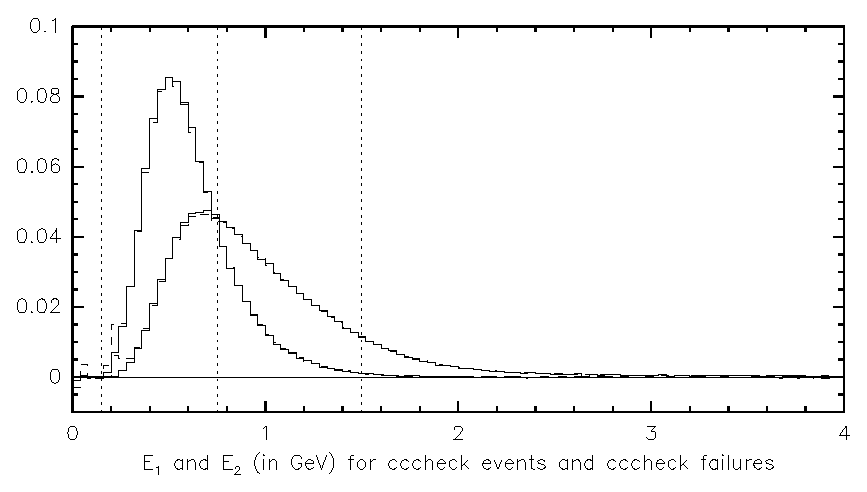
\includegraphics[width=\linewidth]{plots/trigger_neutralpart}
  \end{center}
  \caption{\label{trigger_neutralpart} Biggest and second-biggest
    shower energies in cccheck events (solid) and cccheck failures
    (dashed).  (All cccheck failures satisfy database filters.)  The
    CBLO (0.15 GeV), CBMD (0.75 GeV), and CBHI (1.5 GeV) thresholds
    are indicated by dotted lines.}
\end{figure}

The measured probabilities are in agreement, but their uncertainty is
large for the $\Upsilon(3S)$, which has the largest
continuum-subtraction.  Both the $\Upsilon(2S)$ and $\Upsilon(3S)$ are
open to cascade decays (into $\Upsilon$ and $\chi_b$), so I would
expect their trigger efficiencies to be similar, as it is in the Monte
Carlo.  Therefore, I will apply the $\Upsilon(2S)$ CC trigger
uncertainty to $\Upsilon(3S)$ data and obtain the following errors on
hadronic trigger efficiency: 0.45\% for the $\Upsilon(1S)$, 0.91\% for
the $\Upsilon(2S)$ and $\Upsilon(3S)$.  These errors are sums of the
data--Monte Carlo discrepancies and the data uncertainties in
quadrature.  Another error, from the DR simulation, will be applied to
this.

One might argue that these specially-chosen events have sculpted
shower energy distributions.  This is shown to be not true in Figure
\ref{trigger_neutralpart}: the two biggest showers (which are the only
ones that matter for triggering) have the same distributions in
cccheck events as in other $\Upsilon$ decays.

\subsection{Uncertainty in DR Simulation}

Unfortunately, I cannot perform the same study for the tracking part
of the trigger because no unbiased all-neutral trigger line exists for
CLEO-III.  Instead, I will reproduce the Monte Carlo simulation in a
way that I can control, and vary the input (within uncertainties) to
verify that the trigger response is largely unaffected.

My Toy Monte Carlo has the following algorithm.
\begin{enumerate}

  \item Randomly choose a ``number of quality tracks'' from an input
    distribution.  The distribution from the Full Monte Carlo is
    presented on the far left of Figure \ref{trigger_toymcexamples}.

  \item Randomly choose a ``number of CBLO clusters'' and a ``number
    of CBMD clusters.''  The distributions from which \#CBLO and
    \#CBMD are chosen depend on the given number of quality tracks, to
    try to reproduce some of the correlations exhibited by real
    events.  This is why the number of quality tracks is picked first:
    it best characterizes the event type.  The middle of Figure
    \ref{trigger_toymcexamples} shows two sample \#CBMD distributions,
    one for 0-track events and another for 4-track events.

    The CBLO clusters and CBMD clusters are not correlated with each
    other, but in the Toy Monte Carlo \#CBLO $<$ \#CBMD happens only
    0.18\% of the time.

  \item Randomly choose a ``number of AXIAL tracks.''  This, too,
    depends on the number of quality tracks.  The far right of Figure
    \ref{trigger_toymcexamples} shows the AXIAL track distributions
    given four quality tracks from the Full Monte Carlo and from data.
    By swapping input distributions, I will find the trigger's
    sensitivity to data--Monte Carlo differences.

  \item Randomly choose a ``number of STEREO tracks,'' given a number
    of AXIAL tracks.  This should be tied to AXIAL tracks rather than
    quality tracks to account for the large correlation between these
    two variables.

  \item Construct a trigger decision out of \#CBLO, \#CBMD, \#AXIAL,
    and \#STEREO, and repeat 100,000 times.  This will be
    enough to calculate the trigger efficiency to an uncertainty of
    0.03\%.  All trigger efficiencies quoted from the Toy Monte Carlo
    have this same small uncertainty.

\end{enumerate}

\begin{figure}[t]
  \begin{center}
    \includegraphics[width=\linewidth]{plots/trigger_toymcexamples}
  \end{center}
  \vspace{-1.3 cm}
  \caption{\label{trigger_toymcexamples} A few sample distributions
    which are used by the Toy Monte Carlo.  Left: \#quality tracks
    from the Full Monte Carlo.  Middle: \#CBMD distributions from the
    Full Monte Carlo, given zero quality tracks (solid) or four
    quality tracks (dotted).  Right: \#AXIAL distributions from the
    Full Monte Carlo (solid) and data (dotted), each for 4 quality
    tracks.}
\end{figure}

All tests will be performed with the Toy Monte Carlo, so differences
in trigger efficiency should be measured relative to the Toy Monte
Carlo with default inputs, not the Full Monte Carlo.  Yet I need to
know how well the Toy Monte Carlo reproduces the Full Monte Carlo, so
this will be my first comparison test.  The default input
distributions (\#quality tracks, \#CBLO, etc.) for the Toy Monte Carlo
are taken from the Full Monte Carlo, so this test only determines how
much is lost by not fully simulating events in the Toy Monte Carlo.
Any difference between the default Toy Monte Carlo and the Full Monte
Carlo will be taken as a systematic error, which will be applied once
to the trigger uncertainty.  The following comparison yields
differences less than 0.14\%.
\begin{center}
  \begin{tabular}{l c c c}
    & $\Upsilon(1S)$ & $\Upsilon(2S)$ & $\Upsilon(3S)$ \\\hline
    Full MC & 99.68\% & 99.44\% & 99.50\% \\
    Toy MC (default) & 99.67\% & 99.54\% & 99.64\% \\
  \end{tabular}
\end{center}

The second test estimates sensitivity to track-finding errors in the
trigger.  While the default Toy Monte Carlo gets its \#AXIAL tracks
and \#STEREO tracks from the Full Monte Carlo, the ``get trigger
tracks from data'' variant uses distributions extracted from raw data.
These raw data were not selected for a particular event type, so they
contain bhabha events as well as hadrons, but only in the two-quality
track column.  These data were also filtered by the trigger itself.
Events with zero AXIAL tracks exist in the sample (from the
BarrelBhabha trigger line) but there are very few one-AXIAL track
events.  Nevertheless, associating AXIAL track distributions with a
hadronic number of quality tracks distribution should unfold these
distortions.

As an alternate method, I derived another \#AXIAL tracks distribution
from the Full Monte Carlo, but tuned it to look like data.  The
\#AXIAL track distributions in data tend toward slightly lower values
than those in the Full Monte Carlo, which is to say that the AXIAL
track finding efficiency is lower in data than it is in Monte Carlo.
For an example of this, see the far right of Figure
\ref{trigger_toymcexamples}; the dotted data distribution is smeared
8.3\% lower than the solid Full Monte Carlo distribution (every
twelfth track is dropped).  To generate this distribution, I apply the
following convolution to the Full Monte Carlo \#AXIAL track
distribution:
\begin{equation}
  t'(n) = \sum_{k=0}^\infty t(n+k)
  \left(\begin{array}{c} n+k \\ n
  \end{array}\right) (1 - p)^n p^k
  \label{trigger_trackconvolutioneqn}
\end{equation}
where $t(n)$ is the number of tracks distribution before convolution,
$t'(n)$ after, and $p$ = 0.083 is the probability of losing one track.
This will place a more stringent bound on the track-finding systematic
since it will always lower the trigger efficiency, unlike the
data-based method (described in the previous paragraph), which has
competing effects.

In both methods, the maximum deviation is 0.18\%.
\begin{center}
  \begin{tabular}{l c c c}
    & $\Upsilon(1S)$ & $\Upsilon(2S)$ & $\Upsilon(3S)$ \\\hline
    Toy MC (default) & 99.67\% & 99.54\% & 99.64\% \\
    Get trigger tracks from data & 99.56\% & 99.42\% & 99.49\% \\
    Drop every 12$^{\mbox{\scriptsize th}}$ AXIAL track from MC & 99.50\% & 99.36\% & 99.47\%
  \end{tabular}
\end{center}

The third and fourth tests estimate sensitivity to charged particle
multiplicity and to track reconstruction efficiency.  As can be seen
in the cascades study (Figure \ref{cascades_tracks}), the Monte Carlo
generally underestimates the number of quality tracks.  This could be
because the Monte Carlo generates too few charged particles or because
the Monte Carlo has too low of a track reconstruction efficiency, or
too many Monte Carlo tracks fail track quality cuts (equivalent to
reconstruction efficiency).  The third test will be to swap the Monte
Carlo's quality track distribution for one from data, and the fourth
test will be to vary the track finding efficiency in the Monte Carlo.

To swap the Monte Carlo's quality track distribution for one from
data, I need only read values off of Figure \ref{cascades_tracks}.
There is one caveat: the $\Upsilon(1S)$ represented in the cascades
study is boosted and can suffer from track confusion with the two
pions.  Therefore, I must first replace the \#quality tracks
distribution from the Full Monte Carlo with one from the cascade Monte
Carlo.  This is also read off of Figure \ref{cascades_tracks}; it is
the solid histogram.

The number of tracks distribution from data is not perfectly known,
and it would be good to propagate this uncertainty.  In particular,
the trigger is most sensitive to the number of 0- and 1-track events.
A second \#quality tracks distribution was derived from data, which
has the 0- and 1-track bins raised by 1$\sigma$ in uncertainty.  The
maximum deviation in this study was 0.43\%.
\begin{center}
  \begin{tabular}{l c c c}
    & $\Upsilon(1S)$ & $\Upsilon(2S)$ & $\Upsilon(3S)$ \\\hline
    Toy MC (default) & 99.67\% & 99.54\% & 99.64\% \\
    Get \#quality tracks from cascade MC & 99.77\% & & \\
    Get \#quality tracks from cascade data & 99.87\% & & \\
    Raise 0- and 1-track bins 1$\sigma$ in data & 99.44\% & & \\
  \end{tabular}
\end{center}

To vary the quality track finding efficiency in the Monte Carlo (the
fourth and last test), I will use the convolution defined in Equation
\ref{trigger_trackconvolutioneqn} and its approximate inverse:
\begin{equation}
  t(n) \approx \frac{t'(n) - t'(n+1)(n+1)p}{1 - np}\mbox{.}
\end{equation}
(This was derived by keeping only first-order terms in $p$ and solving
a recurrence relation.)  Track reconstruction efficiency is in
agreement between data and Monte Carlo to at least 2\%
[\ref{cite:trackeff}], so I set $p$ = 0.02 and calculate
\begin{center}
  \begin{tabular}{l c c c}
    & $\Upsilon(1S)$ & $\Upsilon(2S)$ & $\Upsilon(3S)$ \\\hline
    add 2\% more tracks & 99.69\% & 99.61\% & 99.67\% \\
    Toy MC (default) & 99.67\% & 99.54\% & 99.64\% \\
    drop 2\% of tracks & 99.69\% & 99.53\% & 99.64\%.
  \end{tabular}
\end{center}
All deviations are smaller than the uncertainty of 0.03\%, so this
last test contributes no systematic error.

The systematic errors from these four tests, along with the
uncertainty in the CC simulation from the last Subsection, are
presented in Table \ref{trigger_finalerrors}.  The total error is
0.71\% for $\Upsilon(1S)$ and 1.07\% for $\Upsilon(2S)$ and
$\Upsilon(3S)$, mostly due to uncertainty in the CC simulation.

\begin{table}[p]
  \caption{\label{trigger_finalerrors} Summary of all systematic
    errors in trigger efficiencies for $\Upsilon$ events.  Arrows
    indicate systematic errors which were copied from one resonance to
    another.}
  \begin{center}
    \begin{tabular}{l c c c}
      & $\Upsilon(1S)$ & $\Upsilon(2S)$ & $\Upsilon(3S)$ \\\hline
      Uncertainty in CC simulation             & 0.45\% & 0.91\% & $\longrightarrow$ \\
      Uncertainty in DR simulation             &        &        &        \\
      \mbox{\hspace{0.5 cm}} difference between Full MC and Toy MC      & 0.03\% & 0.10\% & 0.14\% \\
      \mbox{\hspace{0.5 cm}} trigger track-finding (convolution method) & 0.17\% & 0.18\% & 0.17\% \\
      \mbox{\hspace{0.5 cm}} \#quality tracks MC $\to$ cascade MC       & 0.10\% & $\longrightarrow$ & $\longrightarrow$ \\
      \mbox{\hspace{0.5 cm}} \#quality tracks from data                 & 0.10\% & $\longrightarrow$ & $\longrightarrow$ \\
      \mbox{\hspace{0.5 cm}} raise 0- and 1-track bins in data          & 0.43\% & $\longrightarrow$ & $\longrightarrow$ \\
      \mbox{\hspace{0.5 cm}} quality track finding efficiency           & 0.04\% & 0.08\% & 0.04\% \\\hline
                                               & 0.66\% & 1.04\% & 1.04\%
    \end{tabular}
  \end{center}
\end{table}

\subsection{Cross-check: Plotting Low-Level Trigger Variables} \label{trigger:subsection_lowlevel}

One last way to confirm that 0.7--1\% is a reasonable uncertainty to
place on the trigger efficiency is to extract low-level trigger
variables from the unfiltered dataset.  In addition to being free from
cuts, re-processing raw data allowed me to access \#AXIAL tracks,
\#STEREO tracks, \#CBLO clusters, and \#CBMD clusters directly.
Therefore, I can plot them in data and overlay Monte Carlo for a
comparison.

In Figures \ref{trigger_lowlevel_1s}, \ref{trigger_lowlevel_2s}, and
\ref{trigger_lowlevel_3s}, I present the four low-level trigger
variables for the $\Upsilon(1S)$, $\Upsilon(2S)$, and $\Upsilon(3S)$,
respectively.  Data have been continuum-subtracted,
beam-gas-subtracted, and cosmic ray-subtracted, and only hadronic
decays are shown.  (Leptonic decays have been left out of the Monte
Carlo, and the Monte Carlo lepton samples have been used to subtract
the leptonic modes from the data.)  Because the data must have passed
the trigger decision, the same requirement is applied to the Monte
Carlo.  (Unfiltered Monte Carlo is overlaid with dotted lines, but
these lines are hardly distinguishable from the filtered Monte Carlo
histograms.)

\begin{figure}[p]
  \begin{center}
    \includegraphics[width=\linewidth]{plots/trigger_lowlevel_1s}
  \end{center}
  \caption{\label{trigger_lowlevel_1s} Low-level trigger variables for
    $\Upsilon(1S)$ hadronic decays passing the trigger, from data
    (cross-hairs) and Monte Carlo (histograms).  Dashed lines indicate
    cut thresholds, and dotted histograms are Monte Carlo without the
    trigger cut.}
\end{figure}

\begin{figure}[p]
  \begin{center}
    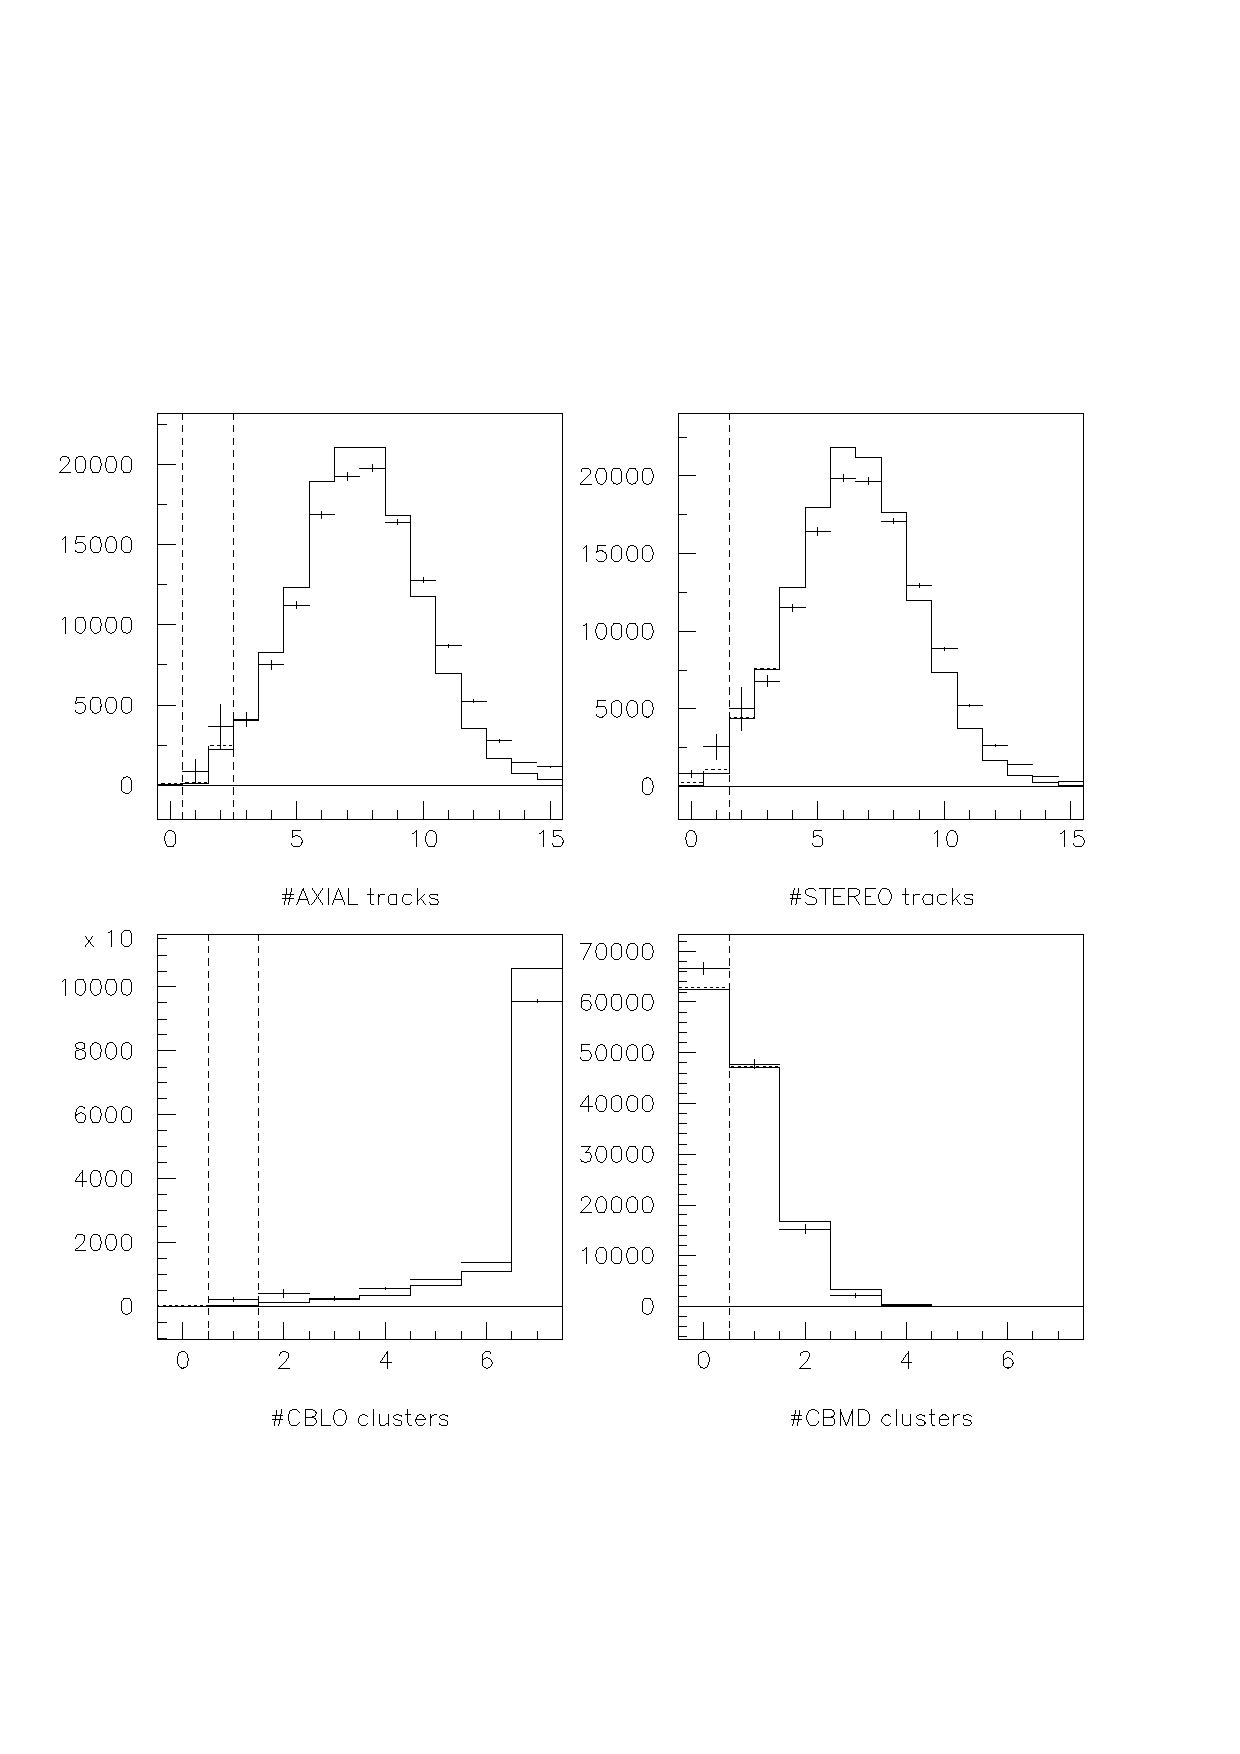
\includegraphics[width=\linewidth]{plots/trigger_lowlevel_2s}
  \end{center}
  \caption{\label{trigger_lowlevel_2s} Low-level trigger variables for
    $\Upsilon(2S)$ hadronic decays passing the trigger, from data
    (cross-hairs) and Monte Carlo (histograms).  Dashed lines indicate
    cut thresholds, and dotted histograms are Monte Carlo without the
    trigger cut.}
\end{figure}

\begin{figure}[p]
  \begin{center}
    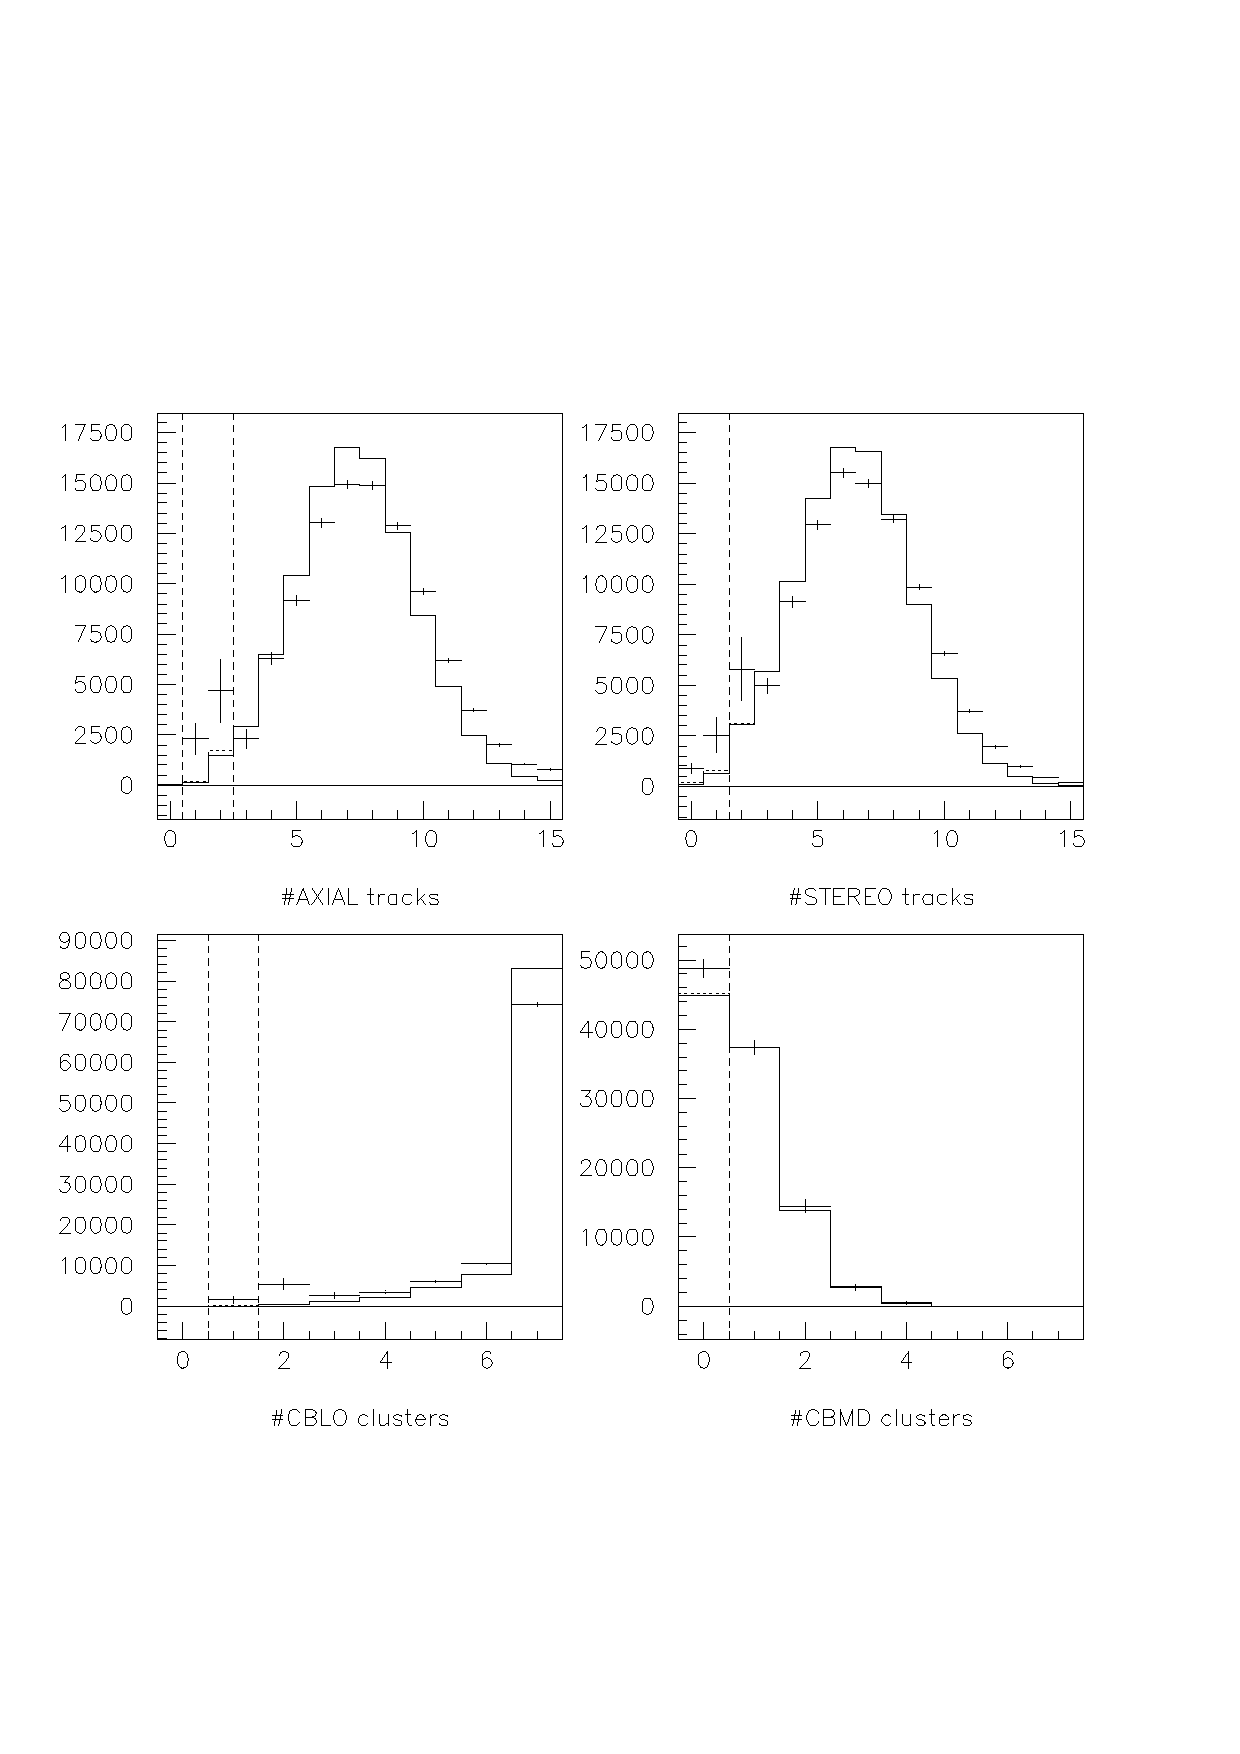
\includegraphics[width=\linewidth]{plots/trigger_lowlevel_3s}
  \end{center}
  \caption{\label{trigger_lowlevel_3s} Low-level trigger variables for
    $\Upsilon(3S)$ hadronic decays passing the trigger, from data
    (cross-hairs) and Monte Carlo (histograms).  Dashed lines indicate
    cut thresholds, and dotted histograms are Monte Carlo without the
    trigger cut.}
\end{figure}

Four discrepancies are apparent: the number of tracks distribution is
wider and higher in data, there are more CBLO clusters in the Monte
Carlo (7 is an overflow bin), there are fewer zero-CBMD events in the
Monte Carlo, and the $\Upsilon(1S)$ and $\Upsilon(3S)$ also have fewer
two-CBLO events in the Monte Carlo.

The number of quality tracks distributions in cascade data and cascade
Monte Carlo have the same discrepancy as the one seen here (Figure
\ref{cascades_tracks}), so the error is more likely to be due to the
generator's charged multiplicity distributions than modeling of DR hit
response.

The CC cluster discrepancies may all be symptoms of incorrectly
simulating the way a Monte Carlo shower is partitioned into tiles.
The two-CBLO bin, in data, is highly correlated with \#CBMD in such a
way that indicates that many showers are on the border between being
recognized as one CBMD or two CBLO.  This same correlation is present
in the Monte Carlo, but to a much lesser degree, which accounts for
both the zero-CBMD bin and the two-CBLO bin being low.  The Monte
Carlo's overestimate of \#CBLO may be due to the same error.

However, these discrepancies are easily overwhelmed by the systematic
errors I have already placed on the trigger efficiency.  Considering
that the trigger inefficiency, as measured in Monte Carlo, is 0.2\%
and 0.4\% (for the $\Upsilon(1S)$, and for the $\Upsilon(2S)$ and
$\Upsilon(3S)$, respectively), the errors I have assumed are
approximately three times the size of the effect.  The advantage of
the complete study is that I have been able to account for the
possibility that the Monte Carlo isn't simply missing a large source
of inefficiency.  Because these comparisons with data must be done
after the trigger has already filtered the events, such a possibility
could sneak through a simple data--Monte Carlo comparison.

\section{Efficiency of the Trigger for Event Type Gamgam}

Unlike hadronic decays of the $\Upsilon$, where the completeness of
the Monte Carlo has to be checked, gamgams are theoretically
well-understood.  This gives me freedom to measure gamgam cut
efficiencies in any order, so I choose to measure the trigger
efficiency after all other cuts have been applied.

My gamgam count is not going to be used to determine the total
integrated luminosity of all scans, but the integrated luminosity
ratios from one run to another.  Therefore, I am only interested in
how gamgam's trigger efficiency changes from run to run.  This is not
something I can learn from the Monte Carlo; I will need to find a way
to derive this information from the data.

BarrelBhabha, the trigger used for gamgams, requires two CBHI
clusters, one on either side of the CC barrel (one on the east and one
on the west).  There is also a very weak $\phi$ back-to-back
requirement, but it is easily satisfied by my events, especially after
I impose a strict back-to-back requirement.  BarrelBhabha suffers an
inefficiency at $\cot\theta$ = 0 (the center of the barrel) because
both CBHI clusters may be detected on the same side of the CC barrel,
due to measurement error.  This can be hard to predict, so I avoid
that region with a $|\cot\theta|$ minimum.

As its name suggests, bhabhas also satisfy the BarrelBhabha trigger.
This allows me to measure the trigger efficiency by collecting bhabhas
on a different trigger line (Hadron or RadTau or ElTrack) and then
asking if the bhabha event also satisfies BarrelBhabha.  The event
selection for bhabhas depends almost entirely on tracking
requirements, and the ElTrack trigger line is independent of
BarrelBhabha systematics inasmuch as tile inefficiencies don't appear
symmetrically on both sides of the detector.  To measure trigger
efficiency given the other gamgam cuts, each bhabha event is
additionally subjected to all gamgam cuts except
\begin{itemize}
  \item BarrelBhabha trigger line,
  \item zero quality tracks, and
  \item $|\sin(\phi_1 - \phi_2)|$ $<$ 0.04 (showers back-to-back
    in $\phi$).
\end{itemize}
The last requirement is only satisfied by particles that don't bend in
the detector's magnetic field.  The $\phi$ back-to-backness of bhabhas
is limited by a cut on \eisr.

An initial measurement of BarrelBhabha trigger efficiency revealed
holes in $\theta$ and $\phi$ that were present for different run
periods.  These holes were excluded in the gamgam cuts (and,
subsequently, the bhabhas which are used to measure BarrelBhabha
efficiency).  These are the first two ``reject'' lines in gamgam's
definition in Table \ref{cuts:eventtypes}.  A third region was
rejected because Surik Mehrabyan discovered a pair of mis-mapped
cables, which were later fixed (this could, in principle, affect the
trigger efficiency measurement).  With these restrictions, almost all
efficiencies are now 99.8\%.  Eleven outliers were investigated in the
CLEO-III e-log: most of them had ``CC trigger stripes in phi''
comments.  I have rejected these runs and listed them in Table
\ref{datasets:badruns} as having ``gamgam trigger issues.''  The final
plot of trigger efficiency versus run is in Figure
\ref{trigger_gamgam_vrun}.

The scatter in this plot is almost entirely due to statistical error.
If the number of standard deviations from the mean are plotted in a
histogram (a ``pull'' distribution, Figure \ref{trigger_gamgam_hist}),
the Gaussian width is 1.12.  The uncertainties in hadronic
cross-section will be dominated by the gamgam count, not the bhabha
correction (because bhabhas far outnumber gamgams), so there is no
harm in leaving this correction in.

\begin{figure}[p]
  \begin{center}
    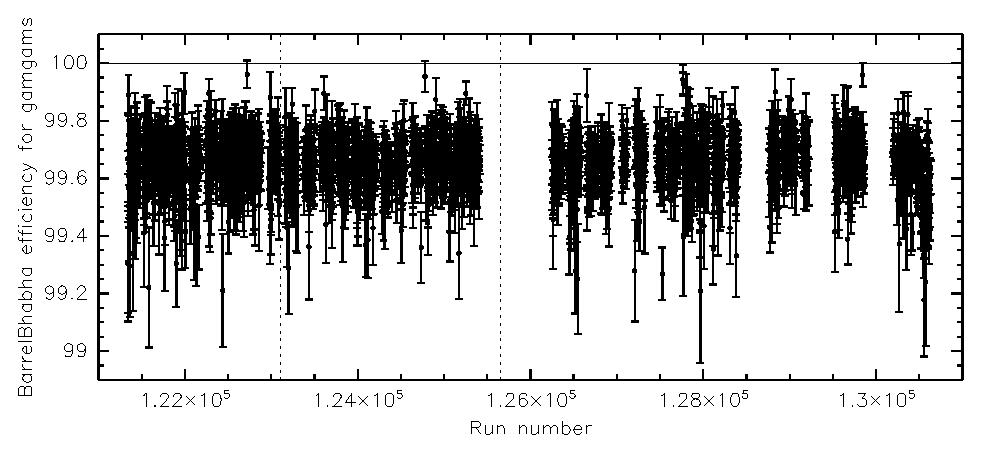
\includegraphics[width=\linewidth]{plots/trigger_gamgam_vrun}
  \end{center}
  \caption{\label{trigger_gamgam_vrun} BarrelBhabha trigger efficiency
  for gamgams, given gamgam cuts.  Dotted lines separate
  $\Upsilon(3S)$, $\Upsilon(1S)$, and $\Upsilon(2S)$ (from left to
  right).}
\end{figure}

\begin{figure}[p]
  \begin{center}
    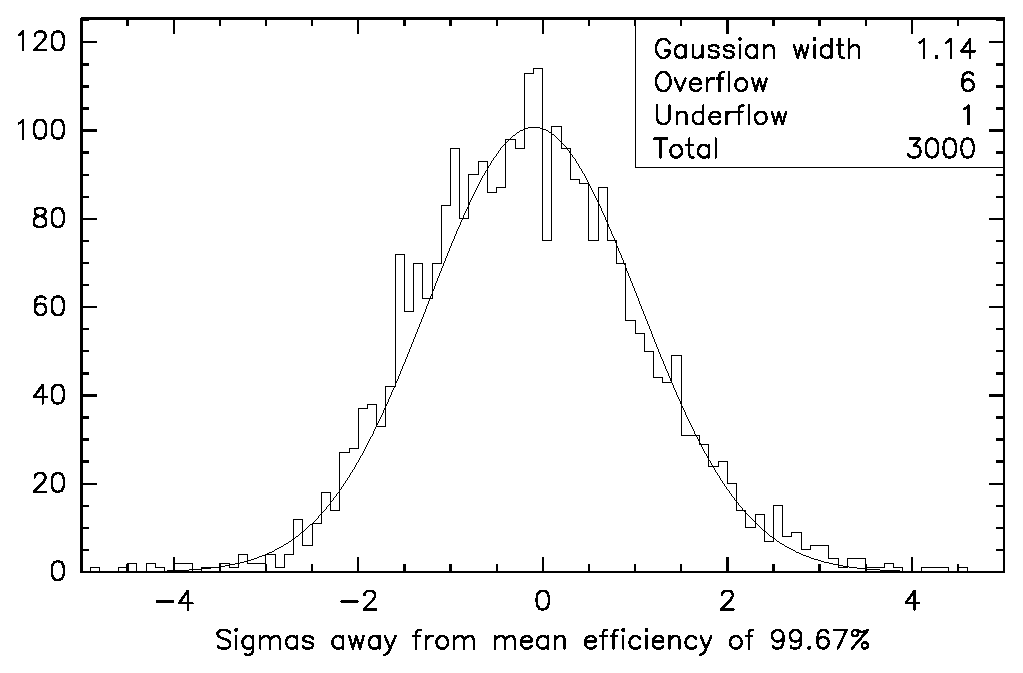
\includegraphics[width=\linewidth]{plots/trigger_gamgam_hist}
  \end{center}
  \caption{\label{trigger_gamgam_hist} Standard deviations from
    average BarrelBhabha efficiency in number of sigmas (pull
    distribution).  Each entry is a run from the database dataset.}
\end{figure}


%% \chapter{Signal Efficiency}
%% Until now, I haven't been explicit about my definition of ``signal.''
Ultimately, $\Gamma_{ee}$ will be derived from the total integrated
$\Upsilon$ cross-section, so in that sense, every $\Upsilon$ decay is
my signal.  However, leptonic final states ($e^+e^-$, $\mu^+\mu^-$,
and $\tau^+\tau^-$, but not cascades that might contain leptons)
should be suppressed to avoid large continuum subtractions and
possible systematics due to interference with these modes.  In fact,
the quantity which is most often quoted in place of $\Gamma_{ee}$ is
$\Gamma_{ee}\Gamma_\subs{had}/\Gamma_\subs{tot}$, which is derived
from the integrated hadronic cross-section.  (Here, ``hadronic
cross-section'' means all modes other than leptonic final states.)

To translate from $\Gamma_{ee}\Gamma_\subs{had}/\Gamma_\subs{tot}$ to
$\Gamma_{ee}$, one multiplies by a factor of
\begin{equation}
  \frac{\Gamma_\subs{tot}}{\Gamma_\subs{had}} = \frac{1}{1 - 3
  \mathcal{B}_{\mu\mu}}  \mbox{ (assuming lepton universality).}
\end{equation}
This process is exactly the same as defining all $\Upsilon$ decays as
the signal and using Monte Carlo to correct for missing leptonic
modes.  Nevertheless, I'm going to stick with tradition and define all
non-leptonic decay modes of $\Upsilon$ to be my signal, and $\Upsilon
\to e^+e^-$, $\mu^+\mu^-$ as backgrounds.  The third leptonic mode,
$\Upsilon \to \tau^+\tau^-$, is 57\% efficient for the cuts that
define event type hadron.  It could therefore be considered a large
background, but it {\it is} part of what I will be adding back in
later.  Furthermore, I can't simply subtract it, as it has complicated
interference behavior through the resonance scan.  I treat it,
therefore, as a second signal.

I do not often make this distinction between signal and leptonic modes
in comparisons of data and Monte Carlo.  In comparing two histograms, I
could leave the leptons in the data and in the Monte Carlo, or I could
use the Monte Carlo to subtract them from the data.  Both of these
result in exactly the same comparison.  Therefore, I will usually
leave the leptons in the data when I am only comparing with Monte
Carlo.  (The only place in this paper where I did remove leptons from
data is in Subsection \ref{trigger:subsection_lowlevel}.)

\section{Measurement Technique}

My technique for measuring hadronic efficiencies will be as follows.
\begin{enumerate}

  \item Trigger: I have set a 0.66\%, 1.04\%, 1.04\% error on the
    Monte Carlo's estimate of this (which is essentially 100\%).

  \item \dxy: The cascades study tells me that I can trust the Monte
    Carlo for this cut, within 0.15\% ``validity uncertainty.''  (See
    Table \ref{cascades_contributions}.)  The looseness of this cut
    suggests that I can apply the same 0.15\% to the $\Upsilon(2S)$
    and $\Upsilon(3S)$.

  \item \dz: Same thing except that the validity uncertainty is
    0.48\%.

  \item \pone: The validity uncertainty is 0.35\% for hadronic decays.
    This cut strongly discriminates between cascades to leptons and
    all other hadronic decays, so I will want to break the Monte Carlo
    up into different modes and propagate uncertainties from branching
    fractions.

  \item \visen: Limitations in the cascades study prohibit me from
    applying the same technique.  I instead add a cascades
    measurement of very low visible energy (0--30\% \ecom) to an
    unfiltered-dataset measurement of low visible energy (30--40\%
    \ecom) for a total cut efficiency.

  \item \lfourdec: This is highly efficient after all cuts, so I
    simply count surviving events from the unfiltered dataset.

\end{enumerate}

After visually checking for data/Monte Carlo discrepancies, I will
read off the efficiency of cuts \#1--\#4 from Monte Carlo, vary
branching fractions in the Monte Carlo, and then add to the error the
validity uncertainties I determined from cascades.  The efficiency of
the \visen\ cut given \#1--\#4 will be measured using the
cascades+unfiltered data technique, and then multiplied for the total
efficiency of cuts \#1--\#5.  Then I will use the data to show that
the last cut has negligible impact.

This means that I am not a priori trusting the Monte Carlo.  The
$\Upsilon(1S)$ efficiency doesn't really depend on the Monte Carlo at
all: the validity uncertainties derived from the cascades study is the
difference between the true efficiency and the Monte Carlo's estimate.
Likewise, all hadronic decay modes shared by the $\Upsilon(2S)$ and
$\Upsilon(3S)$ ($ggg$, $gg\gamma$, and $q\bar{q}$) are actually tied
to the true $\Upsilon(1S)$ efficiency through these validity
uncertainties.  My assumption is that the $\Upsilon(1S)$ efficiencies
apply to the $\Upsilon(2S)$ and $\Upsilon(3S)$ for non-cascade decays.
For cascade decays, however, I am trusting the Monte Carlo: in
principle, the true $\chi_b$ efficiency might be very different from
the Monte Carlo's estimate.  But I assume that because the Monte Carlo
has successfully reproduced $ggg$ hadronization, it will also
correctly reproduce $gg$ hadronization.

I explicitly trust the Monte Carlo's prediction of all leptonic
efficiencies, including the mode $\Upsilon \to \tau^+\tau^-$.  Only
branching fraction uncertainties are propagated.
 
\section{Overlays of Unfiltered Data and Monte Carlo}

Monte Carlo simulations of $\Upsilon(1S)$ decays were shown to be
consistent with the data in cascade decays, but its validity for
direct $\Upsilon(1S)$ production or for the $\Upsilon(2S)$ or
$\Upsilon(3S)$ has yet to be seen.

Overlays of unfiltered data and Monte Carlo are presented in Figures
\ref{efficiency_dxy}, \ref{efficiency_dz}, \ref{efficiency_p1}, and
\ref{efficiency_visen}.  Cuts were applied cumulatively, so the first
two (\dxy\ and \dz) are significantly distorted by backgrounds.
(Continuum, beam-gas, and cosmic rays have all been subtracted, but
\dxy\ and \dz\ aren't perfectly represented by the single- and no-beam
samples.)  That is why these first two cuts are very loose: to bolster
confidence in the predicted efficiency of the cut in the face of large
backgrounds.  Only special classes of signal events which vertex far
from the origin wouldn't be visible in these plots, but the cascades
study would have caught this possibility.  (The ``validity
uncertainties'' are upper limits on these branching fractions.)

\begin{figure}
  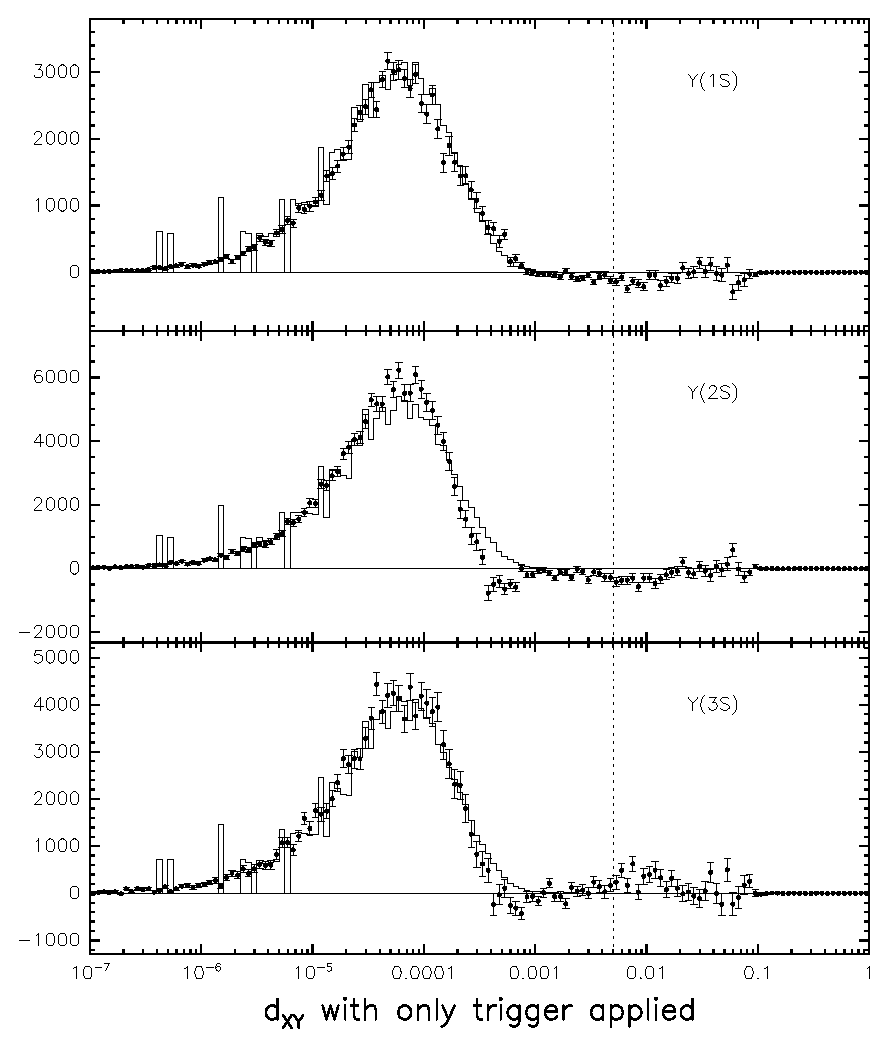
\includegraphics[width=\linewidth]{plots/efficiency_dxy}
  \caption{\label{efficiency_dxy} Closest track to the beamspot in XY,
    presented in log $x$ scale, for the three resonances (data with
    errorbars), compared with Monte Carlo (solid histogram).  The cut
    boundary is indicated by the dotted line.}
\end{figure}

\begin{figure}
  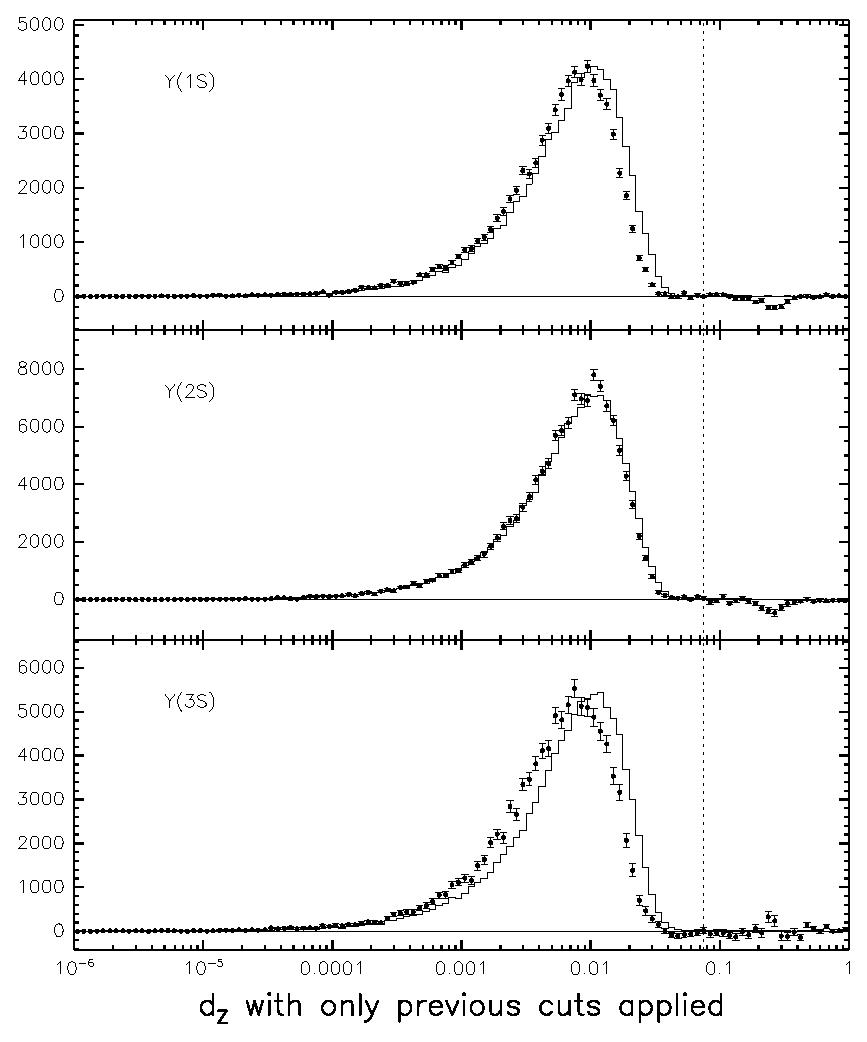
\includegraphics[width=\linewidth]{plots/efficiency_dz}
  \caption{\label{efficiency_dz} Event vertex Z, presented in log $x$
    scale, for the three resonances (data with errorbars), compared
    with Monte Carlo (solid histogram).  The cut boundary is indicated
    by the dotted line.}
\end{figure}

\begin{figure}
  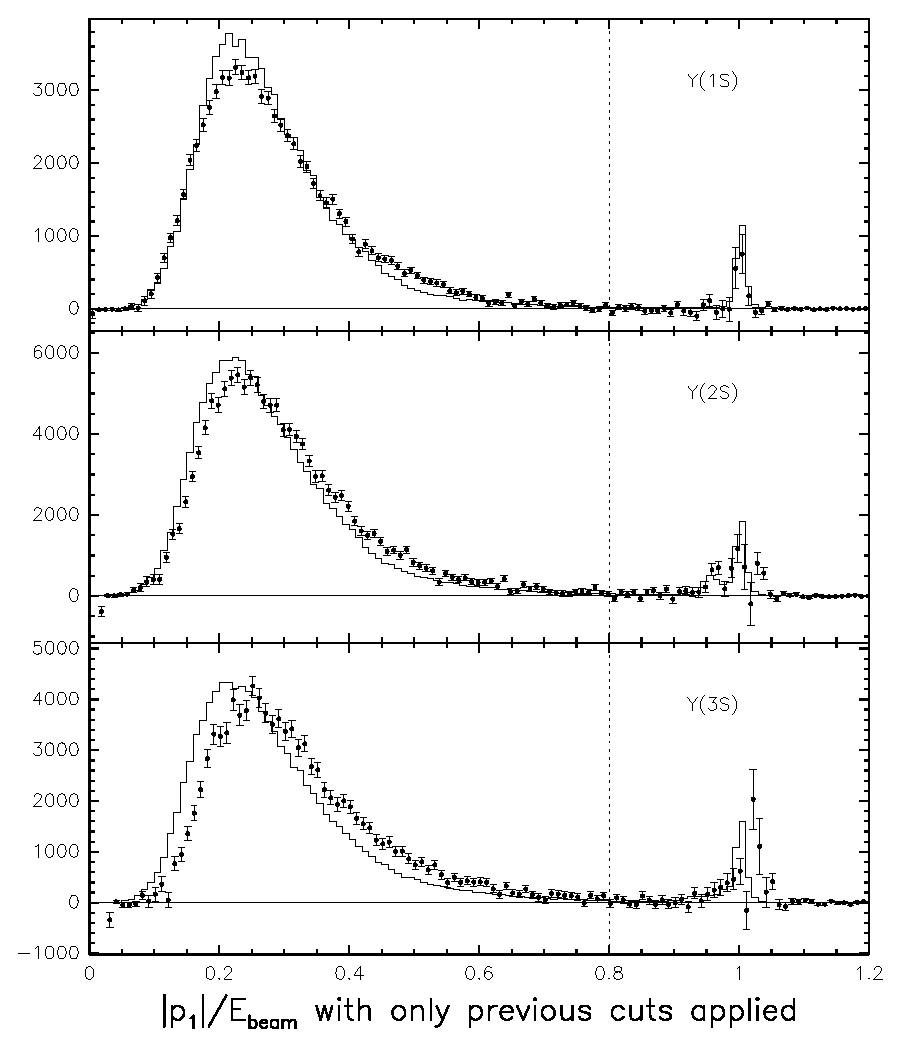
\includegraphics[width=\linewidth]{plots/efficiency_p1}
  \caption{\label{efficiency_p1} Largest track momentum divided by
    \ebeam\ for the three resonances (data with errorbars), compared
    with Monte Carlo (solid histogram).  The cut boundary is indicated
    by the dotted line.}
\end{figure}

\begin{figure}
  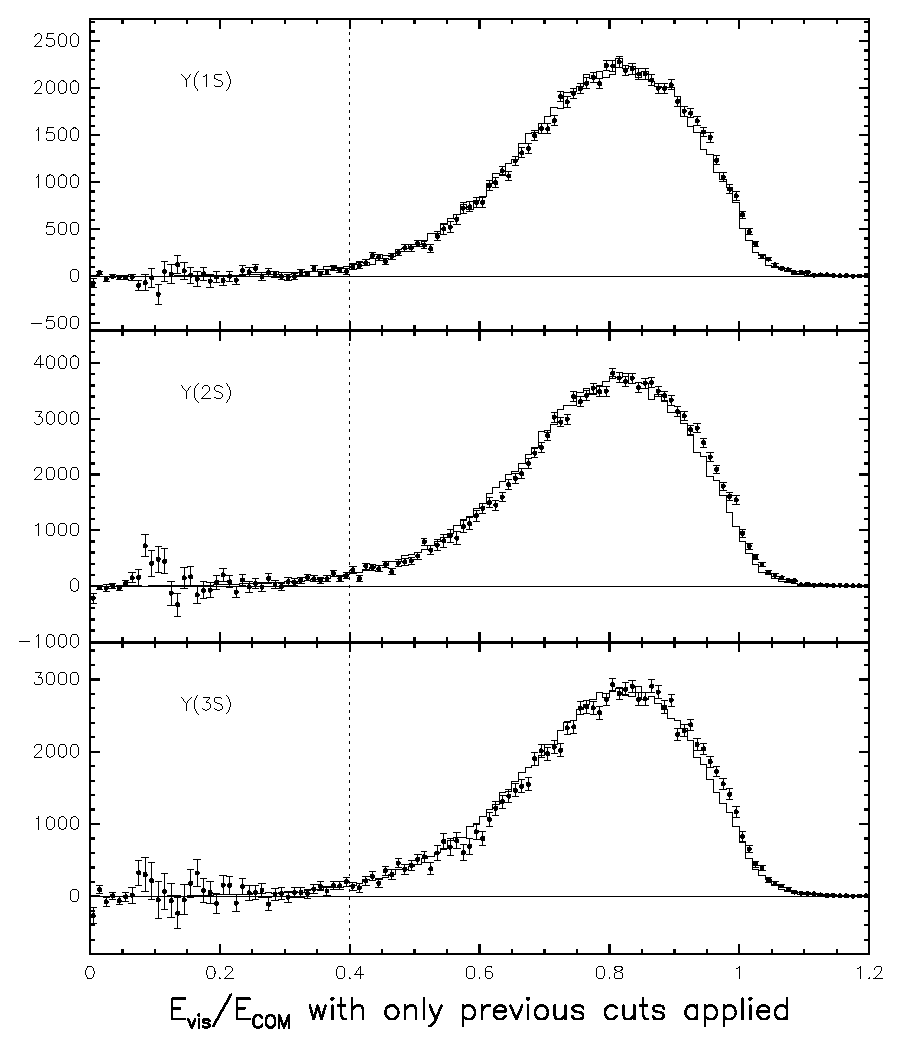
\includegraphics[width=\linewidth]{plots/efficiency_visen}
  \caption{\label{efficiency_visen} Visible energy divided by \ecom\
    for the three resonances (data with errorbars), compared with
    Monte Carlo (solid histogram).  The cut boundary is indicated by
    the dotted line.}
\end{figure}

The third and fourth cuts, \pone\ and \visen, are much tighter, but
can be observed in a low-background environment.  The difference in
the shape of \pone\ from 10\% to 60\% \ebeam\ between data and Monte
Carlo is disturbing.  But it is present in the $\Upsilon(1S)$, and can
even be seen in cascade plots (Figure \ref{cascades_p1}), and yet the
data/Monte Carlo difference is only 0.35\%.  In Figure
\ref{efficiency_overlay}, we see that the three resonances don't seem
to differ in the tail, so the 0.35\% applies to each.  Also in Figure
\ref{efficiency_overlay}, we see that the three resonances have very
similar \visen\ distributions, so they can share a visible energy
correction.

\begin{figure}
  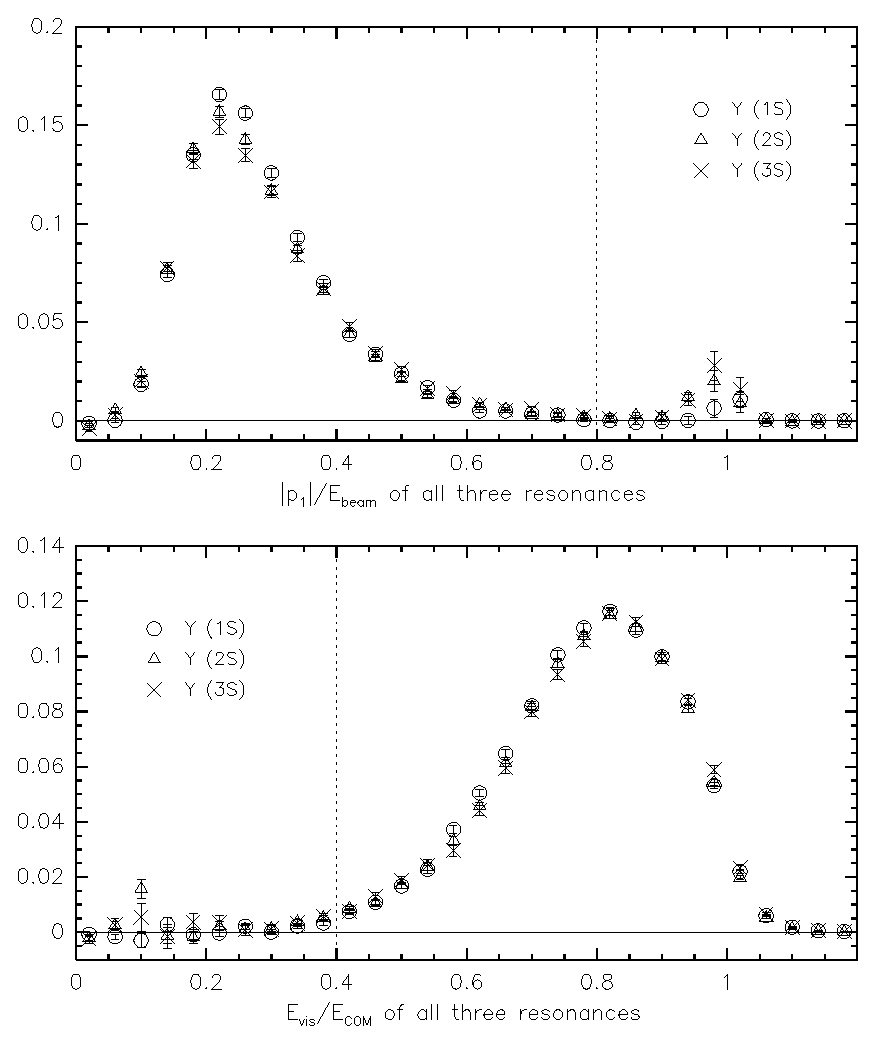
\includegraphics[width=\linewidth]{plots/efficiency_overlay}
  \caption{\label{efficiency_overlay} Largest track momentum (as a
  fraction of \ebeam) and visible energy (as a fraction of \ecom) for
  all three resonances overlaid upon each other, rather than the
  Monte Carlo.  Cut boundaries are indicated by the dotted lines.}
\end{figure}

\section{Cut Efficiencies from Monte Carlo}

The only cut efficiency that will be measured using signal Monte Carlo
is the combination of cuts \#1--\#4 (trigger through \pone).  With the
exception of $\tau^+\tau^-$, all modes are either very efficient or
very inefficient.  This will trivialize the Monte Carlo's dependence
on variations in branching fractions.  The mode-by-mode efficiencies
are listed in Table \ref{efficiency_montecarlo}, and the aggregate
efficiency in Table \ref{efficiency_montecarlo3}.

I used the following to combine the individual mode efficiencies:
\begin{eqnarray}
  \mathcal{B}_{q\bar{q}} &=& R \mbox{ } \mathcal{B}_{\mu\mu} \\
  \mathcal{B}_{\mbox{\scriptsize cascades}} &=& 0 \mbox{ } (1S), \mbox{\hspace{0.25 cm}} 45.4 \pm 1.5\% \mbox{ } (2S), \mbox{\hspace{0.25 cm}} 45.2 \pm 1.5\% \mbox{ } (3S) \\
  \mathcal{B}_{ggg} &=& \frac{1 - (3+R)\mathcal{B}_{\mu\mu} - \mathcal{B}_{\mbox{\scriptsize cascades}}}{1 + \Gamma_{gg\gamma / ggg}} \\
  \mathcal{B}_{gg\gamma} &=& (\Gamma_{gg\gamma/ggg}) \, \mathcal{B}_{ggg}
\end{eqnarray}
The leptonic branching fraction $\mathcal{B}_{\mu\mu}$ was measured to
high precision recently by Istvan Danko, with the values 2.49 $\pm$
0.07\% ($\Upsilon(1S)$), 2.03 $\pm$ 0.09\% ($\Upsilon(2S)$), and 2.39
$\pm$ 0.12\% ($\Upsilon(3S)$) [\ref{cite:istvan}].  The ratio of quark
pairs to muon pairs, $R$, is 3.58 $\pm$ 0.14 [\ref{cite:novoR}].  For
cascade branching fractions, I added together all cascade modes in the
PDG [\ref{cite:pdg}].

There seems to be a discrepancy in the literature regarding the value
of $\Gamma_{gg\gamma}/\Gamma_{ggg}$; a direct measurement
[\ref{cite:cleoggg}] yields 2.75\% $\pm$ 0.16\% and the world-average
of $\alpha_s$ run to $M_\Upsilon$ predicts a value of 3.65\% $\pm$
0.05\% [\ref{cite:pdgggg}], using the formula
\begin{equation}
\frac{\Gamma_{gg\gamma}}{\Gamma_{ggg}} = \frac{36 \, {e_b}^2}{5} \frac{\alpha_{QED}}{\alpha_s(M_\Upsilon)}
\left( 1 + 2.2(6) \, \frac{\alpha_s(M_\Upsilon)}{\pi} + \mbox{\ldots} \right) \mbox{.}
\end{equation}
My value, 3.20 $\pm$ 0.45\%, straddles these two, with an error
large enough to encompass both.

It matters very little what value I use, since the aggregate
efficiency is insensitive to all cut variations, as seen in Table
\ref{efficiency_montecarlo2}.  Included in this table is sensitivity
to a known bug in my Monte Carlo sample (I toggle between unaffected
and all events), sensitivity to code release (the same events were
processed in different code releases), and the statistical error in
the Monte Carlo sample.

\begin{table}[t]
  \caption{\label{efficiency_montecarlo} Monte Carlo efficiencies for
    each mode for cuts \#1--\#4 (up to and including \pone)}
  \begin{center}
    \begin{tabular}{l c c c}
       & $\Upsilon(1S)$ & $\Upsilon(2S)$ & $\Upsilon(3S)$ \\\hline
      $e^+e^-$ & 0.24\% & 0.23\% & 0.28\% \\
      $\mu^+\mu^-$ & 0.16\% & 0.13\% & 0.19\% \\
      $\tau^+\tau^-$ & 77.25\% & 78.66\% & 77.03\% \\
      $ggg$ & 99.75\% & 99.78\% & 99.78\% \\
      $gg\gamma$ & 96.44\% & 96.69\% & 96.44\% \\
      $q\bar{q}$ & 97.99\% & 98.20\% & 98.37\% \\
      cascade $\to e^+e^-$ or $\mu^+\mu^-$ & & 0.90\% & 0.76\% \\
      cascade $\to$ other modes & & 99.53\% & 99.48\% \\
    \end{tabular}
  \end{center}
\end{table}

\begin{table}[p]
  \caption{\label{efficiency_montecarlo3} Aggregate hadronic Monte
    Carlo efficiency for cuts \#1--\#4 (up to and including \pone)}
  \begin{center}
    \begin{tabular}{l c c c}
       & $\Upsilon(1S)$ & $\Upsilon(2S)$ & $\Upsilon(3S)$ \\\hline
      Hadronic efficiency of cuts \#1--\#4 & 99.52\% & 97.92\% & 98.19\% \\
    \end{tabular}
  \end{center}
\end{table}

\begin{table}[p]
  \caption{\label{efficiency_montecarlo2} Hadronic Monte Carlo
    sensitivity to variations in branching fractions and other
    parameters}
  \begin{center}
    \begin{tabular}{l c c c}
       & $\Upsilon(1S)$ & $\Upsilon(2S)$ & $\Upsilon(3S)$ \\\hline
      $\mathcal{B}_{\mu\mu}$ (affects $q\bar{q}$ fraction) & 0.006\% & 0.010\% & 0.012\% \\
      $R$ (affects $q\bar{q}$ fraction)                    & 0.005\% & 0.005\% & 0.005\% \\
      $gg\gamma/ggg$                                       & 0.013\% & 0.006\% & 0.006\% \\
      $\mathcal{B}_\subs{cascades}$                        &         & 0.054\% & 0.044\% \\
      $\mathcal{B}_{ee}$ and $\mathcal{B}_{\mu\mu}$ of lower resonances &         & 0.003\% & 0.003\% \\\hline
      Bunch-finder bug                                      & 0.28\%  & 0.33\%  & 0.19\% \\
      Code release                                         & 0.011\% & 0.002\% & \\
      Finite sample                                        & 0.43\%  & 0.31\%  & 0.31\% \\\hline
      Sum in quadrature                                    & 0.51\%  & 0.46\%  & 0.37\% \\
    \end{tabular}
  \end{center}
\end{table}

\section{Cut Efficiencies from Unfiltered Data}

As can be seen in Figure \ref{efficiency_visen}, there is a great
uncertainty in the 0--30\% \ecom\ region of \visen, because a large
continuum peak is being subtracted there.  This uncertainty is all the
more acute since it is unclear what scale factor $S_c$ to use to
subtract these events, as many of them may be two-photon.  The region
from 30\% to 40\% \ecom\ is less uncertain, and it is here that signal
efficiency begins.  That is why I will measure only this part of the
\visen\ cut efficiency in the unfiltered dataset, leaving the rest for
the cascade dataset, which has substantially less background.

Why not measure the entire cut with cascades?  For one thing, I am
concerned about accepting a 1\% correction to $\Gamma_{ee}$ without
testing it in a non-boosted, $\pi^+\pi^-$-free environment.  Most of
the signal events that fail the \visen\ cut are in the 30--40\% \ecom\
region, so they are accessible to the unfiltered dataset.  By
splitting the measurement into two parts, I obtain a correction which
is consistent with zero from the cascades and a significant correction
from the unfiltered dataset.

The 30--40\% \ecom\ region accounts for 0.52 $\pm$ 0.12\% of the
events in the $\Upsilon(1S)$ plot, 1.01 $\pm$ 0.14\% of the events in
the $\Upsilon(2S)$ plot, and 0.85 $\pm$ 0.21\% of the events in the
$\Upsilon(3S)$ plot.  Toggling cosmic ray and beam-gas backgrounds
only changes the results by 0.01\%, 0.02\%, and 0.10\%, respectively.

Nor is there a significant dependence on ``database partition.''  Most
calibrations are applied to month-long sets of runs called database
partitions: $\Upsilon(3S)$ is split into db16 and db17 (a small part
is in db22, but the unfiltered dataset doesn't include any of these
runs), $\Upsilon(1S)$ is split into db18 and db19 (a small part is in
db17, but again, the unfiltered dataset doesn't include any such
runs), and $\Upsilon(2S)$ is split between db21, db22, db23, db25, and
db27 (the unfiltered dataset distinguishes between runs from db21 and
runs from db23, db25, and db27).  The efficiencies differ between
datasets by 0.22\%, 0.18\%, and 0.25\% for the $\Upsilon(1S)$,
$\Upsilon(2S)$, and $\Upsilon(3S)$.

Another source of systematic error is the fact that the continuum
scale factor, $S_c$, can vary through the plot.  Where the continuum
is dominated by two-photon events, the continuum subtraction should
use 1.005 $\times$ $S_c$, and where it is dominated by everything
else, the continuum subtraction should use $S_c$ as it was calculated
in Chapter \ref{chp:datasets}.  Taking an extreme case, I used 1.005
$\times$ $S_c$ in the 30--40\% \ecom\ region and $S_c$ everywhere
else.  The measurement changed by 0.02\%, 0.05\%, and 0.10\% for
$\Upsilon(1S)$, $\Upsilon(2S)$, and $\Upsilon(3S)$, respectively.

These systematic errors are listed and combined in Table
\ref{efficiency_datapart}.  A branching fraction to events with
\visen\ less than 40\% was obtained by adding the unfiltered dataset
result (30--40\%) to the cascades dataset (0--30\%).  The \visen\ cut
efficiency is the compliment of this.

\begin{table}[t]
  \caption{\label{efficiency_datapart} Summary of the \visen\ cut
    measurement.  Arrows indicate a result from one resonance being
    applied to another.}
  \begin{center}
    \begin{tabular}{l c c c}
       & $\Upsilon(1S)$ & $\Upsilon(2S)$ & $\Upsilon(3S)$ \\\hline
      Branching fraction in 30--40\%      & 0.52\% & 1.01\% & 0.85\% \\\hline
      Statistical error                   & 0.12\% & 0.14\% & 0.21\% \\
      Beam-gas and cosmic rays            & 0.01\% & 0.02\% & 0.10\% \\
      Database partition                  & 0.22\% & 0.18\% & 0.25\% \\
      Continuum-subtraction               & 0.02\% & 0.05\% & 0.10\% \\
      Sum of errors in quadrature         & 0.24\% & 0.23\% & 0.35\% \\\hline
      Branching fraction to 0--30\%       & 0.28 $\pm$ 0.19\% & $\longrightarrow$ & $\longrightarrow$ \\
      Branching fraction to 0--40\%       & 0.80 $\pm$ 0.31\% & 1.29 $\pm$ 0.30\% & 1.13 $\pm$ 0.31\% \\
      Efficiency of \visen\ cut                      & 99.20 $\pm$ 0.31\% & 98.71 $\pm$ 0.30\% & 98.87 $\pm$ 0.31\% \\
      Efficiency from cascades            & 98.90 $\pm$ 0.28\% & & \\
    \end{tabular}
  \end{center}
\end{table}

The last cut, \lfourdec, has an efficiency of of 99.96 $\pm$ 0.03\%,
100.02 $\pm$ 0.03\%, and 100.00 $\pm$ 0.03\% in the unfiltered
dataset.

\section{Putting All the Pieces Together}

The hadronic efficiency is the efficiency of cuts \#1--\#4 (trigger
through \pone, from Monte Carlo), times the efficiency of cut \#5
(\visen, from cascades and the unfiltered dataset), times the
efficiency of cut \#6 (\lfourdec, from the unfiltered dataset).  This
efficiency is given in Table \ref{efficiency_finaltable}.  It incurs
errors from trigger efficiency, verification with cascades, the Monte
Carlo uncertainties on cuts \#1--\#4, the data uncertainties on cut
\#5 and on cut \#6.  All of these errors are summarized in Table
\ref{efficiency_finaltable2}.

\begin{table}[p]
  \caption{\label{efficiency_finaltable} Calculation of the total
    hadronic efficiency}
  \begin{center}
    \begin{tabular}{l c c c}
      & $\Upsilon(1S)$ & $\Upsilon(2S)$ & $\Upsilon(3S)$ \\\hline
      Efficiency of cuts \#1--\#4 (trigger through \pone) & 99.52\% &  97.92\% &  98.19\% \\
      Efficiency of cut \#5 (\visen)                      & 99.20\% &  98.71\% &  98.87\% \\
      Efficiency of cut \#6 (\lfourdec)                   & 99.96\% & 100.02\% & 100.00\% \\\hline
      Total hadronic efficiency                           & 98.68\% &  96.68\% &  97.08\% \\
    \end{tabular}
  \end{center}
\end{table}

\begin{table}[p]
  \caption{\label{efficiency_finaltable2} Calculation of total
    hadronic efficiency error.  Arrows indicate a result from one
    resonance being applied to another.}
  \begin{center}
    \begin{tabular}{l c c c c}
      & $\Upsilon(1S)$ & $\Upsilon(2S)$    & $\Upsilon(3S)$    & source table \\\hline
     Trigger                      & 0.66\% 	       & 1.04\%            & 1.04\%            & \ref{trigger_finalerrors} \\
     Verification with cascades   & 0.61\% 	       & $\longrightarrow$ & $\longrightarrow$ & \ref{cascades_contributions} \\
     Monte Carlo uncertainties    & 0.51\% 	       & 0.46\%            & 0.37\%            & \ref{efficiency_montecarlo2} \\
     \visen\ uncertainties        & 0.31\% 	       & 0.30\%            & 0.31\%            & \ref{efficiency_datapart} \\
     \lfourdec\ uncertainty       & 0.03\% 	       & 0.03\%            & 0.03\%            & \\\hline
     Sum in quadrature            & 1.08\%             & 1.33\%            & 1.30\%            & \\
    \end{tabular}
  \end{center}
\end{table}

Now for the second signal efficiency: $\Upsilon \to \tau^+\tau^-$.
The Monte Carlo claims a 57.8\% efficiency, and that is what I will
believe.  Since $\Upsilon \to \tau^+\tau^-$ represents a 0.578
$\times$ 2\% fraction of the data, even a 10\% uncertainty is
completely negligible.  A later cross-check will make use of a
``quality tracks $>$ 4'' cut: for this I will need to know that 3.8\%
of $\tau^+\tau^-$ survive such a cut.


%% \chapter{Search for Gamgam Backgrounds} \label{chp:gamgambkgnds}
%% Luminosity in the database dataset will be measured with gamgams
because $e^+e^-$ and $\mu^+\mu^-$ are both final states of the
$\Upsilon$.  But can any $\Upsilon$ decays pass gamgam cuts?  Gamgam
requires two large, back-to-back showers, and $\Upsilon \to
\gamma\gamma$ is forbidden by angular momentum conservation.  But
$\chi_{b0}$ and $\chi_{b2}$ are $J^{PC}$ = $0^{++}$ and $2^{++}$
particles, respectively, and can therefore decay to $\gamma\gamma$.
One can imagine, then, a cascade in which the $\Upsilon$ radiates a
small photon to become a $\chi_b$, and then the $\chi_b$ decays into
two large, back-to-back photons.  Such an event would pass gamgam cuts
because gamgam does not exclude a small third photon.

To check for this possibility, I searched the database dataset for
events of this type.  In $\Upsilon(2S)$ and $\Upsilon(3S)$
on-resonance and off-resonance data, I plotted the third largest
shower energy (\ethree) for all events that satisfy gamgam cuts in
Figure \ref{gamgam_chibkgnd}.  The lowest energy a $\Upsilon \to
\chi_b$ cascade photon can have is 60 MeV, so I used gamgam events
with \ethree\ $<$ 60 MeV to scale the off-resonance sample.  Rather
than subtracting on- and off-resonance, I have overlaid them.  Monte
Carlo for this decay chain has also been overlaid (with an arbitrary
normalization) to show where \ethree\ peaks can be expected.  (The
Monte Carlo includes $\chi_{b1}$ in the cascade chain.)  No peaks are
seen in data in the right places.  The differences between on- and
off-resonance distributions are due to variations in noise that do not
affect gamgam counting.

\begin{figure}
  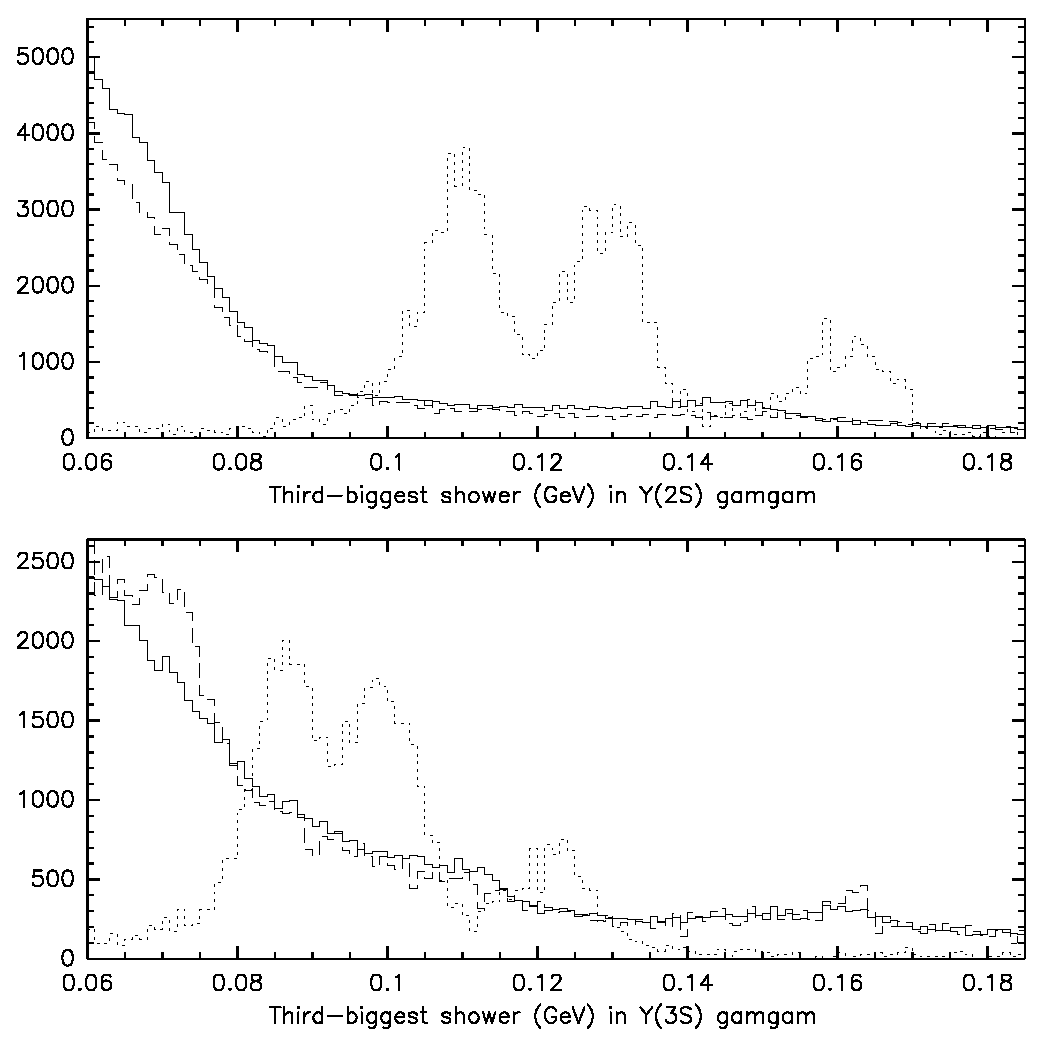
\includegraphics[width=\linewidth]{plots/gamgam_chibkgnd}
  \caption{\label{gamgam_chibkgnd} Energy of the third-largest shower
    in gamgam events.  On-resonance data are solid, scaled
    off-resonance data are dashed, and $\Upsilon \to \gamma
    \chi_{b0,1,2} \to \gamma \gamma \gamma$ Monte Carlo are dotted.}
\end{figure}

Since the database dataset is insensitive to this decay mode, any bias
due to $\gamma\gamma\gamma$ events must be smaller than statistical
errors in the luminosity measurement.  I will ignore its contribution.


%% \chapter{Run-by-Run Dependence of Hadronic Cross-Section}
%% Hadron counting is based almost exclusively on DR cuts and gamgam
counting is based exclusively on CC cuts, so the ratio of these two,
the hadronic cross-section, can be wrong if one system is
unresponsive.  As described in Chapter \ref{chp:cuts}, I have
developed a way to check for failures of DR sensitivity while the CC
is still taking data, and a way to check for failures of CC
sensitivity while the DR is still taking data.

\section{Checking for DR Failures}

``Trackless bhabha'' counts events that look like
gamgams except that the two large showers are not exactly back-to-back
in $\phi$: the two particles that generated the showers must be
deflected from exact collinearity by the magnetic field.  Figure
\ref{runbyrun_trackless0} presents this variable for gamgams and
bhabhas.  The zero-track constraint is also stricter than it is for
gamgams, as not even non-quality tracks or even AXIAL tracks are
allowed.  (Trigger line ElTrack, which requires 1 AXIAL track and 1
CBMD (already guaranteed by BarrelBhabha), is refused.)  The number of
events that satisfy these criteria may be compared with the number of
events with the no-tracks cut released: this is the fraction of real
bhabhas, pointing into the barrel, that fail to generate tracks in the
DR.  I will call this the trackless bhabha fraction.

It is possible that some of the trackless bhabhas counted are actually
radiative gamgams, but the bhabha rate is sufficiently large that this
method is still useful for finding DR failures.  Most runs have a
trackless bhabha fraction of about 0.11\%, so the gamgam background
must be at most this large.  If the trackless bhabha fraction is
$x$\%, then the DR failed to find tracks somewhere between
$(x-0.11)$\% and $x$\%.  For typical statistical errors in the
hadronic cross-section of 2--10\%, a 0.11\% uncertainty in the DR
sensitivity is negligible.

The trackless bhabha fraction is plotted in Figure
\ref{runbyrun_trackless} for all runs in the database dataset.
Twenty-five outliers were identified as having DR problems by the
following method.  Every run was divided into 100 equal time slices,
and the number of trackless bhabhas were counted for each hundredth of
a run.  If any run had more than 80\% of its trackless bhabha events
in the same time slice (usually the first or the last), that run was
identified as having DR problems.  This method identified all the
apparent outliers in Figure \ref{runbyrun_trackless}.

\begin{figure}[p]
  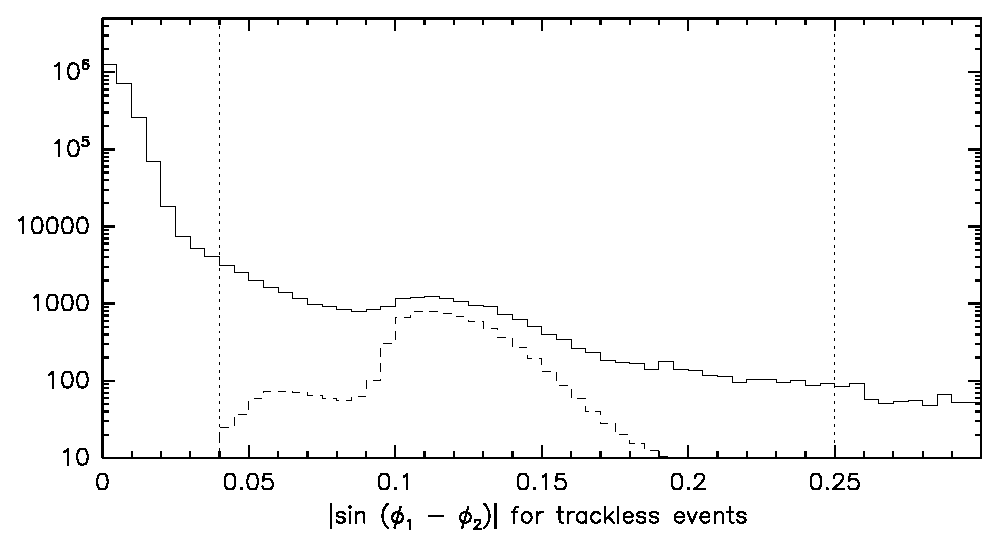
\includegraphics[width=\linewidth]{plots/runbyrun_trackless0}
  \caption{\label{runbyrun_trackless0} Back-to-backness in $\phi$ of
    two largest showers, in events with zero tracks.  The large peak at
    zero are gamgams and the little bump at 0.11 are trackless bhabhas.
    The dashed line shows two-track bhabhas for comparison, and the
    dotted lines are the cut boundaries for trackless bhabhas.}
\end{figure}

\begin{figure}[p]
  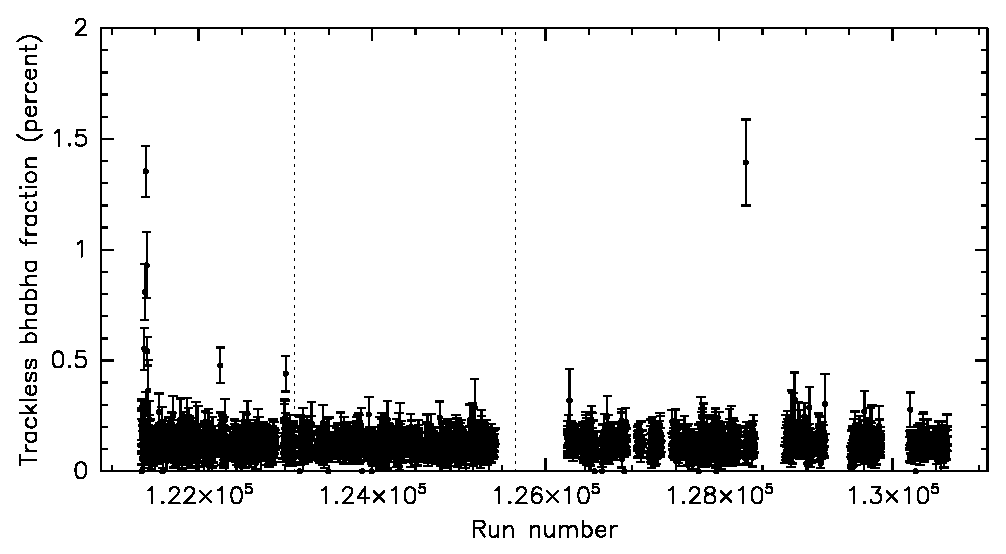
\includegraphics[width=\linewidth]{plots/runbyrun_trackless}
  \caption{\label{runbyrun_trackless} Trackless bhabha fraction (as a
  percent) for every run in the database dataset.  Dotted lines
  separate $\Upsilon(3S)$, $\Upsilon(1S)$, and $\Upsilon(2S)$ (left to
  right).}
\end{figure}

Of these twenty-five outliers, ten are scan runs, which are too
valuable to this analysis to lose.  Therefore, these ten runs were
retained and the other fifteen were rejected before plotting Figure
\ref{runbyrun_trackless}.  (The rejected runs are listed in Table
\ref{datasets:badruns}.)  All of the ten scan runs that had DR
problems had them in the last one-hundredth of the run, as seen in
Figure \ref{runbyrun_trackless2}.  When I count hadrons and gamgams
for these runs, I must count them in only the first 99\% of the run.

\begin{figure}[p]
  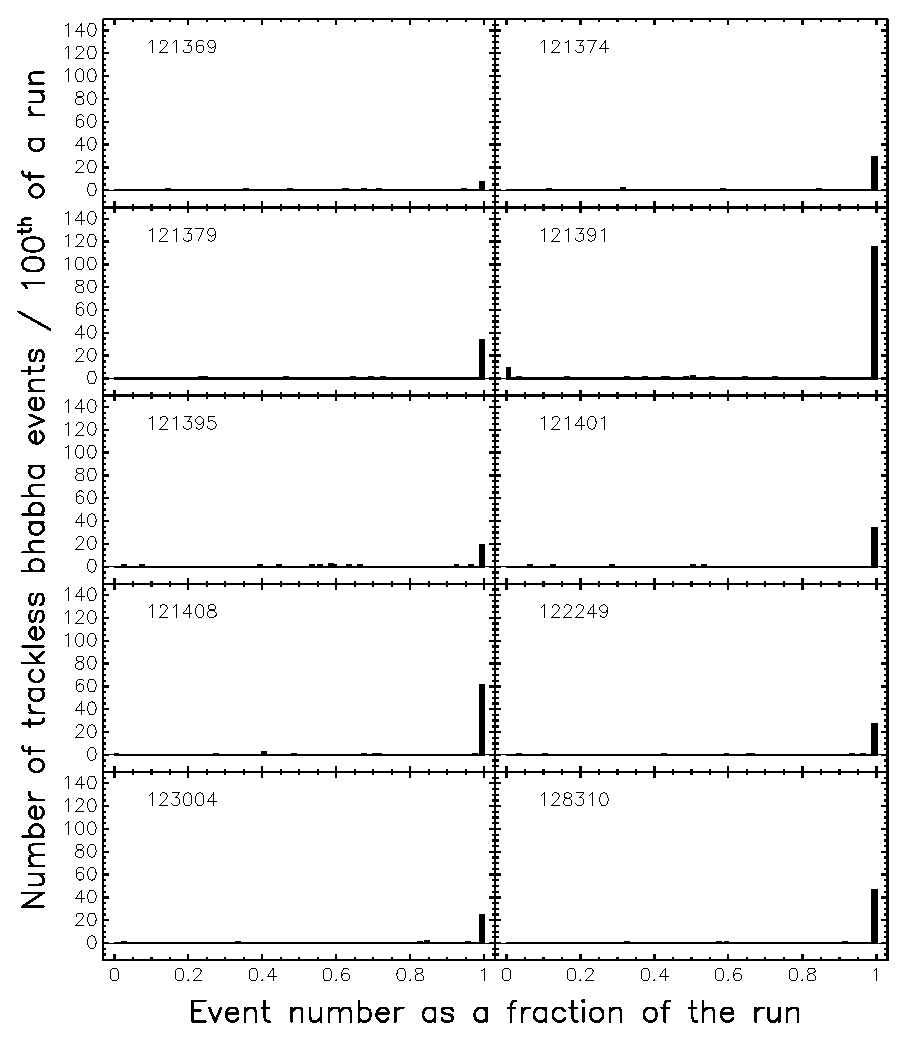
\includegraphics[width=\linewidth]{plots/runbyrun_trackless2}
  \caption{\label{runbyrun_trackless2} Number of trackless bhabhas
  throughout the run for the eight outliers in Figure
  \ref{runbyrun_trackless}.  Histograms are shaded black for
  visibility.}
\end{figure}

\section{Checking for CC Failures}

To check for CC failures, I created the event types DR-trigger bhabha
and DR-trigger mupair.  Both of these require the TwoTrack trigger
only, in order to be independent of the CC, and are built from the
same set of track requirements.  The only difference between these two
event types (and the only reference to a CC variable) is that the
DR-trigger bhabhas require \etwo\ $>$ 40\% \ebeam\ (which is loose)
and DR-trigger mupairs require \etwo\ $<$ 1 GeV.  (These are
non-overlapping criteria.)  This way, if the CC fails, bhabhas will be
identified as mupairs.

The $e^+e^-$ rate, given these cuts, is 13 to 19 times the
$\mu^+\mu^-$ rate, depending on whether the run is on the
$\Upsilon(1S)$ resonance (which contributes fractionally more to the
$\mu^+\mu^-$ rate than to the $e^+e^-$ rate) or in the continuum.
Therefore, a 13\% excess in the ratio
\begin{equation}
  \frac{\mbox{\#DR-trigger mupair}}{\mbox{\#DR-trigger bhabha +
  \#DR-trigger mupair}}
\end{equation}
is a 1\% limit on the fraction of time that the CC is insensitive.
This is because the denominator is independent of CC sensitivity and
CC failures add bhabhas to the mupair count.  I will call this ratio
the mupair fraction.

The mupair fraction is plotted for every run in the database dataset
in Figure \ref{runbyrun_bhamutt}.  No outliers are apparent, but the
statistical uncertainty is too large to place a tight and rigorous
limit on CC failures.  The excess ``mupairs'' in a given run is at
most about 50\%, which translates to a 4\% upper limit on the fraction
of time that the CC is insensitive in a given run.  This is comparable
with the statistical error in hadronic cross-section for a typical
run.

\begin{figure}[p]
  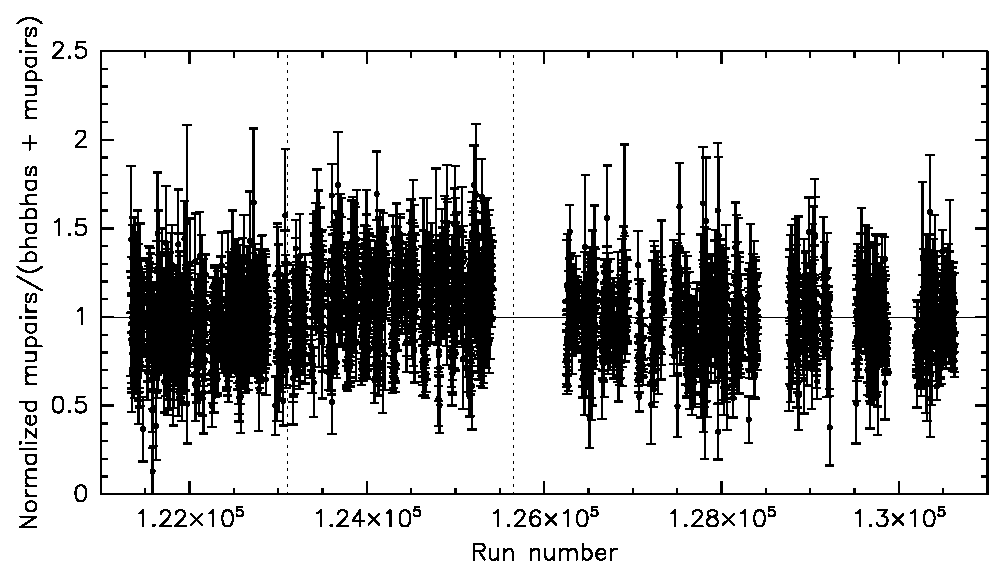
\includegraphics[width=\linewidth]{plots/runbyrun_bhamutt}
  \caption{\label{runbyrun_bhamutt} The mupair fraction, normalized to
  have a weighted mean of 1.0, plotted for every run in the database
  dataset.  Dotted lines separate $\Upsilon(3S)$, $\Upsilon(1S)$, and
  $\Upsilon(2S)$ (left to right).}
\end{figure}

\begin{figure}[p]
  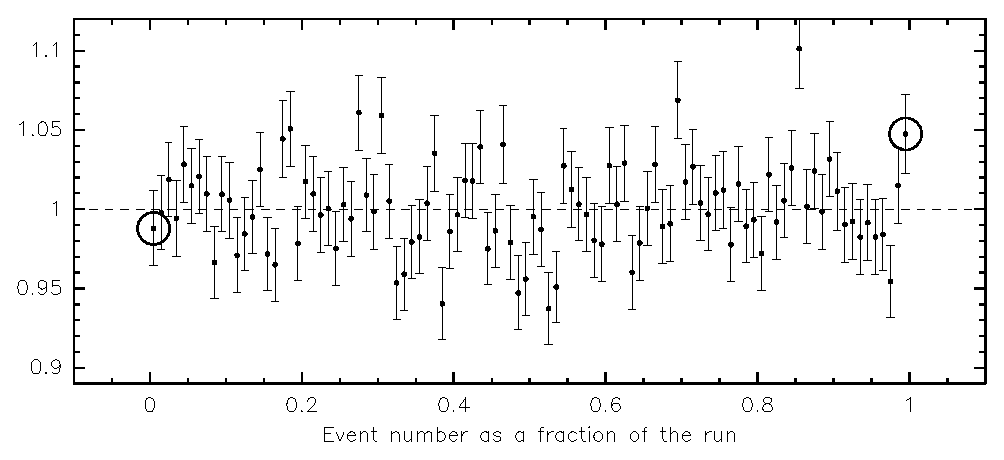
\includegraphics[width=\linewidth]{plots/runbyrun_bhamutt2}
  \caption{\label{runbyrun_bhamutt2} Mupair fraction throughout the
    run, where all runs have been combined.  The first and last bins
    (circled) do not deviate significantly from the average.}
\end{figure}

Assuming, as was the case for DR failures, that detector failure
either happens at the very beginning or the very end of a run, I
plotted the mupair fraction as a function of the run, and combined all
runs together.  In the resulting histogram, the first bin represents
the first hundredth of every run, and the last bin represents the last
hundredth of every run.  If there are CC failures that always happen
at the beginning or the end of the run, they will pile up in these two
bins and I will see a deviation.  The biggest detectable deviations
are 2.7\% for the first hundredth and 5.4\% for the last hundredth
(deviation and uncertainty added in quadrature).  These translate to
0.2\% and 0.4\% limits on the total CC failure rate (good runs
included).  This histogram is plotted in Figure
\ref{runbyrun_bhamutt2}.

Scanning through many of these histograms for individual runs, I did
not see anything peculiar.  I will assume that while the DR can lose
high voltage with the CC still taking data, the CC cannot lose
sensitivity while the DR is still taking data.

\section{Relative Hadronic Cross-section}

Now I am ready to calculate the relative hadronic cross-section.  By
``relative,'' I mean that I will not apply the hadronic efficiency
correction or translate the number of gamgams into an integrated
luminosity in inverse nanobarns: I will just divide the hadron count
by the gamgam count.  I do, however, make corrections that depend on
run number.  The gamgam count has been corrected for BarrelBhabha
trigger efficiency, and the hadron count has been beam-gas-subtracted
(50\% correction with 50\% uncertainty) and cosmic ray-subtracted
(only statistical errors).  In Subsection \ref{runbyrun_ssecvsenergy},
I will also divide by $s$ = \ebeam$^2$ so that hadronic cross-sections
at different energies may be compared.

\subsection{Throughout Each Run}

In presenting relative hadronic cross-sections, I will start at the
most instrumental level and work up to fundamental physics.  First I
plot hadronic cross-section within each run.  Every run was taken at
exactly one beam energy, so this should be constant.  As I did in the
DR and CC tests, I can calculate the hadronic cross-section for each
hundredth of a run, and then perform linear fits to hadronic
cross-section versus time.  The slope of each fit is divided by its
uncertainty and these ``pulls'' are histogrammed in Figure
\ref{runbyrun_hadxs1}-a.  The average slope is zero with only
statistical deviations.  The $\chi^2$ of the linear fits is another
way to spot misshapen distributions: the reduced $\chi^2$ for all the
fits is histogrammed in Figure
\ref{runbyrun_hadxs1}-b.  The average reduced $\chi^2$ is low, but
this may be an effect propagated from low-statistics bins in the
gamgam versus time histograms.

Before drawing these histograms, two outlying runs were identified:
their hadronic cross-section versus time plots are shown in Figure
\ref{runbyrun_hadxs2}.  They have been removed from the dataset.

\begin{figure}[p]
  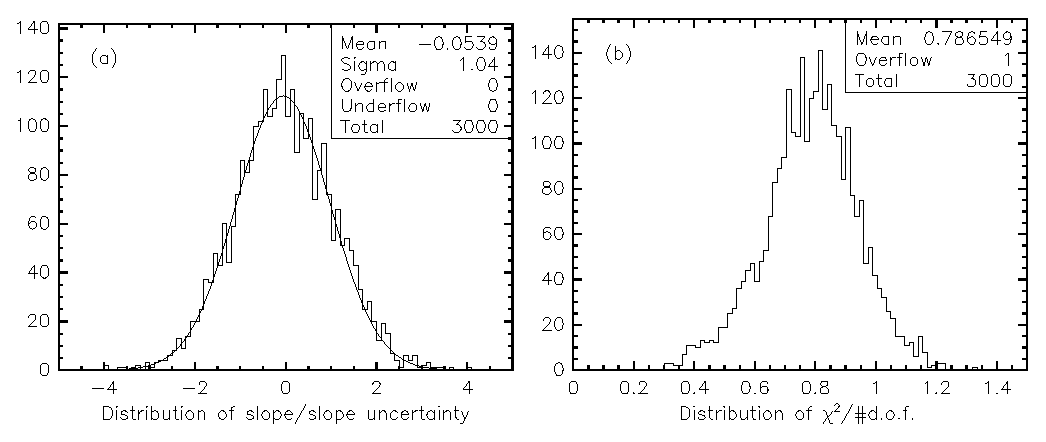
\includegraphics[width=\linewidth]{plots/runbyrun_hadxs1}
  \caption{\label{runbyrun_hadxs1} From left to right: (a) pull
  distribution of slopes in the hadronic cross-section versus time
  fits, as a number of sigmas from zero, and (b) distribution of
  reduced $\chi^2$ for the same fits.  (The outlier is a statistical
  variant.)}
\end{figure}

\begin{figure}[p]
  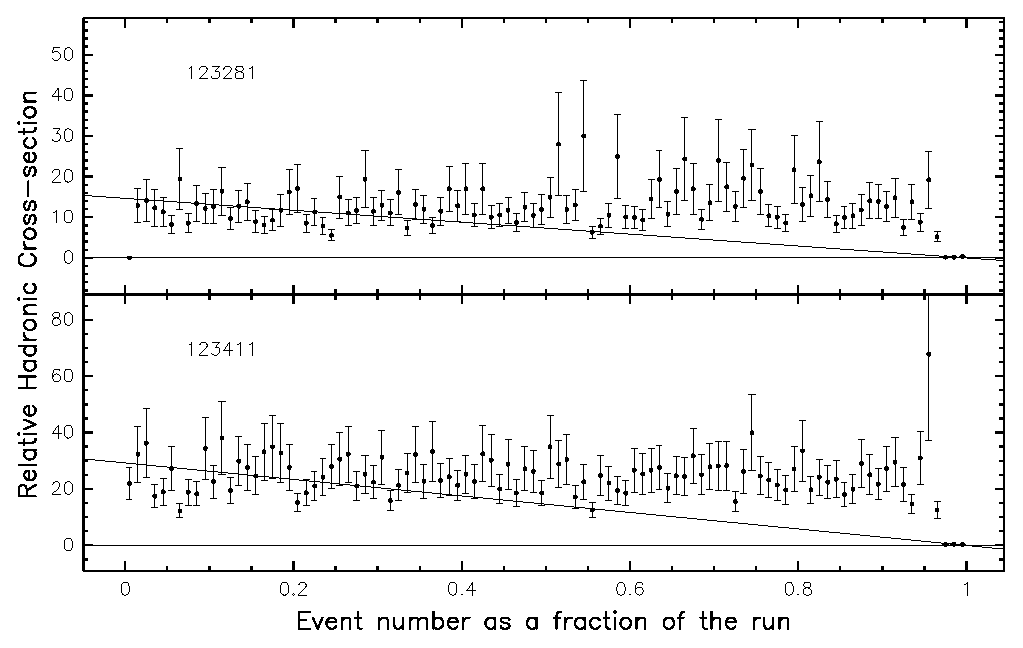
\includegraphics[width=\linewidth]{plots/runbyrun_hadxs2}
  \caption{\label{runbyrun_hadxs2} Two runs that failed to have a
  satisfactory slope (not included in the histograms in Figure
  \ref{runbyrun_hadxs1})}
\end{figure}

\subsection{Run by Run}

Next I will plot the hadronic cross section for each on- and
off-resonance run in the database dataset.  Each of these six samples
(three resonances times on- versus off-resonance) was taken at a
constant beam energy, so the hadronic cross-section should be
constant.  The definition of ``on-resonance'' is a range of energies
only 1.6 MeV wide for each resonance, so this, too, should be
constant.  No $1/s$ correction has been applied in this Subsection, so
continua at the $\Upsilon(1S)$, $\Upsilon(2S)$, and $\Upsilon(3S)$
should all have equal values.  The plots are shown in Figure
\ref{runbyrun_peaksconts}.

\begin{figure}[p]
  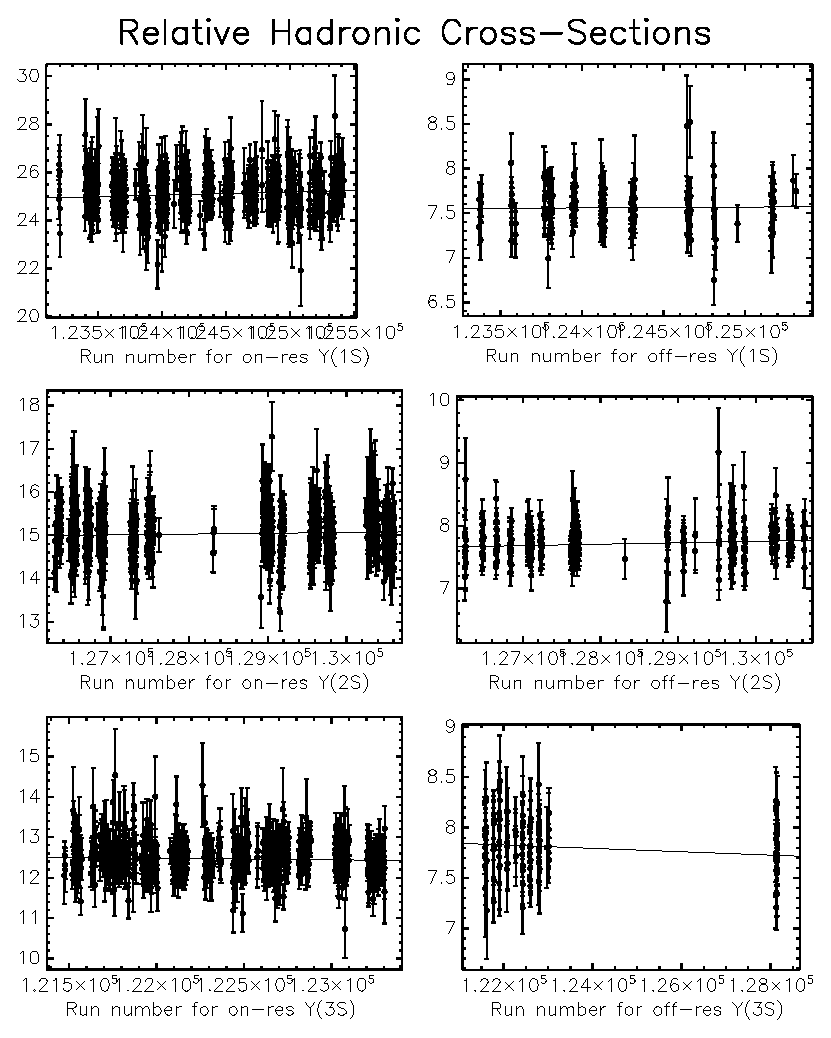
\includegraphics[width=\linewidth]{plots/runbyrun_peaksconts}
  \caption{\label{runbyrun_peaksconts} Relative hadronic cross-section
    versus run number for each of the six constant energies.  A
    straight line has been fitted to each.}
\end{figure}

\begin{figure}[p]
  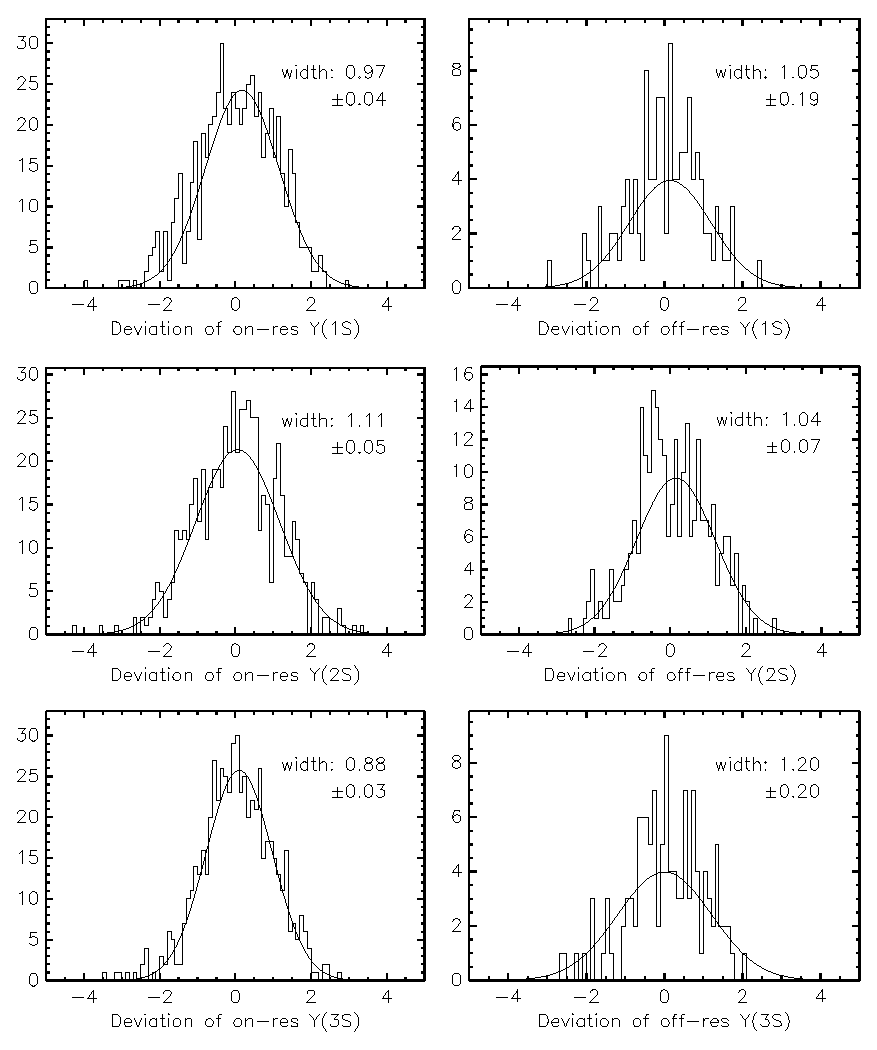
\includegraphics[width=\linewidth]{plots/runbyrun_peaksconts2}
  \caption{\label{runbyrun_peaksconts2} Pull distributions of hadronic
  cross-section in each constant-energy sample.  The widths of fitted
  Gaussians are also displayed.}
\end{figure}

I fitted each constant hadronic cross-section with a straight line.
The significance (value divided by error) of each slope is:
\begin{center}
  \begin{tabular}{c c c c}
    & on-resonance & off-resonance \\
    $\Upsilon(1S)$ & 3.13 & 0.25 \\
    $\Upsilon(2S)$ & 1.76 & 2.45 \\
    $\Upsilon(3S)$ & -1.32 & -1.77. \\
  \end{tabular}
\end{center}
Some of these are marginally significant, so I should try to match
peak and scan data with nearby continuum as much as possible, such
that varying continuum levels are subtracted in a way that cancels the
drift.

Scan and continuum runs aren't always consecutive in the
$\Upsilon(2S)$ dataset, so I will be forced to use continuum from
different eras for a continuum subtraction.  However, at run 127642,
the CC begins to intermittently read out some showers (along the tile
boundaries in the barrel) with higher energies than it should.  This
could raise the hadron count because two-photon events, which are
normally cut out for having too little \visen, may be artificially
raised above the cut threshold.  In fact, combining all $\Upsilon(2S)$
peak and continuum, before and after 127642, I see the peak data raise
2.49 standard deviations (0.078 $\pm$ 0.031 in \#hadrons/\#gamgams
units) and the continuum raise 1.56 standard deviations (0.042 $\pm$
0.027 in the same units).  I will avoid crossing this boundary for
continuum-subtractions.

%% peak
%% (14.991370234331351, 0.024844739090064256)
%% (15.069660152908128, 0.019256898584188539)
%% 0.078 +- 0.031  is 2.49 sigmas

%% cont
%% (7.6884592194542147, 0.020992094512067197)
%% (7.7303710804873385, 0.016947379302405009)
%% 0.042 +- 0.027  is 1.56 sigmas

%% peak bhabha
%% (1.1453608108322908, 0.00069472852035430026)
%% (1.1514073256621737, 0.00053750979311212863)

%% cont bhabha
%% (59.556019903921154, 0.069744336836371058)
%% (59.524565678673258, 0.055778459450481861)
%% 0.031 +- 0.089  is 0.35 sigmas

The $\Upsilon(3S)$ off-resonance dataset has a very large gap before
its last group of runs: extra $\Upsilon(3S)$ was acquired during
$\Upsilon(2S)$ running.  The late $\Upsilon(3S)$ sample includes runs
that are near the peak, but not close enough for my classification.
They have been labeled ``scan'' runs.  I won't mix late $\Upsilon(3S)$
with early $\Upsilon(3S)$.

As a last consistency check, I calculate how far each run is from the
weighted mean of its class as a number of standard deviations.  The
resulting six pull distributions should each be unit Gaussians, and
most of them are, as can be seen in Figure \ref{runbyrun_peaksconts2}.
I cannot explain the narrow width of the $\Upsilon(3S)$.

\subsection{Versus Energy} \label{runbyrun_ssecvsenergy}

Finally, the physics: I will now plot hadronic cross-section as a
function of center-of-mass energy.  To do this properly, I will need
to multiply $\mbox{\#hadrons}/\mbox{\#gamgams}$ by a factor of $1/s$.
The plot of all hadronic cross-sections versus energy is in Figure
\ref{runbyrun_thescans}.  The (nearly) horizontal line on all three
plots is a $1/s$ fit to all continuum data simultaneously; the
$\chi^2/$\#d.o.f. of that fit is 554/525 = 1.06 (an 80\% confidence
level).

There appears to be a distortion in the $\Upsilon(3S)$ lineshape: the
runs responsible for this distortion are all from an era before the
first (intentional) $\Upsilon(3S)$ scan.  In the following Chapter, I
will determine the dates when alterations to the beam energy
calibration are likely to have taken place: the runs responsible for
this distortion may be before the first such calibration, and their
energies therefore can't be determined.  Data like these will not be a
part of any lineshape fit.

\begin{figure}[p]
  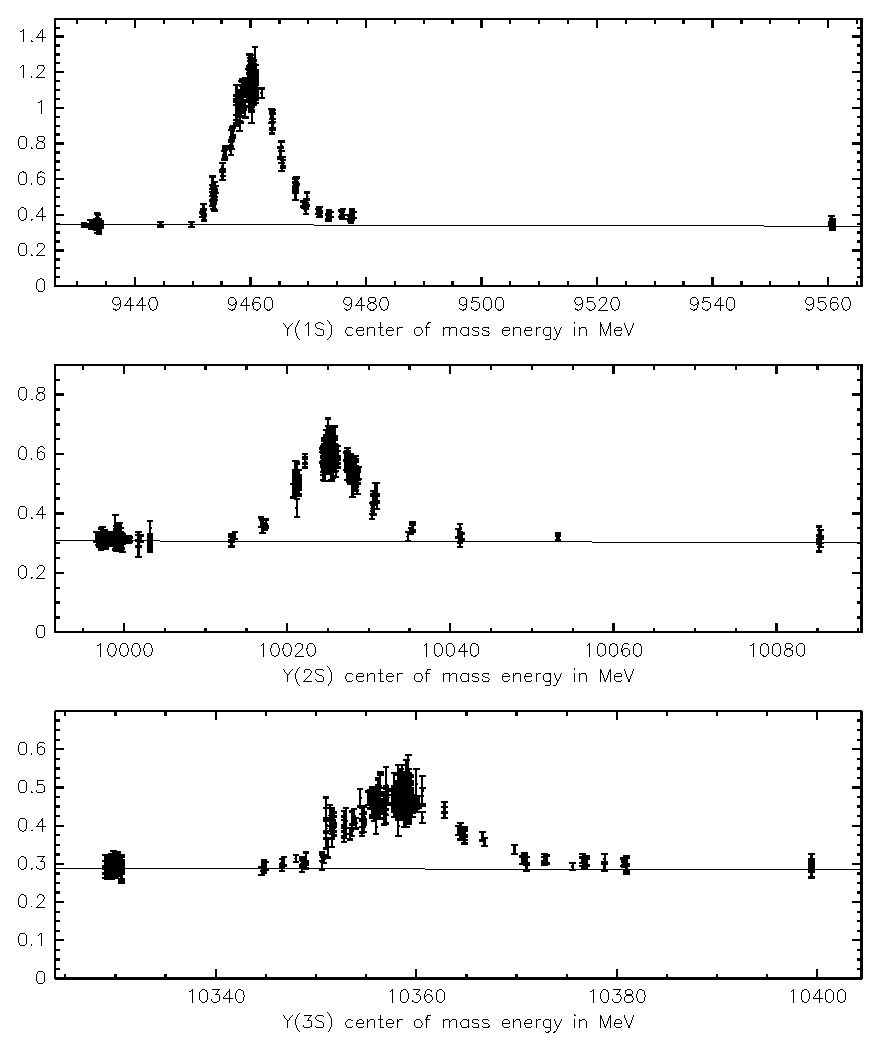
\includegraphics[width=\linewidth]{plots/runbyrun_thescans}
  \caption{\label{runbyrun_thescans} Relative hadronic cross-section
  versus energy reveals the $\Upsilon$ resonance peaks.  The (nearly)
  horizontal line is a $1/s$ fit to all continuum data.}
\end{figure}


\chapter{Lineshape Fitting}
\section{Scan and Fitting Methods}

Each resonance was scanned about ten times: approximately once a week,
CESR's beam energy was varied to independently scan the $\Upsilon$
lineshape.  This is because the measurement of beam energy can't be
guaranteed to its quoted precision from one week to the next, since
the NMR probe that measures it can be displaced during machine
studies, and a fit to lineshape data with unknown energy measurement
errors would be meaningless.  So each of these individual scans is
complete: it can be used to measure $\Gamma_{ee}$ independently.

Fitting each scan independently and then averaging $\Gamma_{ee}$,
however, would not be an optimal use of data.  Some scans don't have a
continuum point (cross-section measurement 20 MeV below the $\Upsilon$
mass), and only one scan at each resonance has a dedicated high-energy
point (20--50 MeV above the $\Upsilon$ mass).  Being far from the
resonance, these measurements aren't sensitive to shifts in beam
energy calibration on the order of an MeV.  (Shifts in apparent beam
energy between individual scans are $\lesssim$1 MeV.)  To optimally
use all the data, each resonance is fitted once with all scans
included, as well as a high-statistics continuum point and a
high-energy point.  Each scan's beam energy calibration is represented
as a floating parameter in the fit.

Each of these three fits allows the continuum background to float
freely: I am not restricting it to any functional form over the
hundreds of MeV from one resonance to the next.  Under a resonance
lineshape (a span of tens of MeV), I will have to assume a given
functional form, and the data are insufficient to let it float in the
fit.






\section{The Scan Periods}

\section{Fitting Continuum Points}

\section{Fitting Each Resonance}

\section{Simulating Beam Energy Calibration Shifts}







%% \chapter{Luminosity Calibration}
%% %% \input{luminosity.tex}

%% \chapter{Conclusion: the Value of $\Gamma_{ee}$}
%% %% \input{conclusion.tex}

%% \appendix

%% \chapter{Files for Monte Carlo Generation} \label{chp:appendixmc}

%% \section{User DECAY.DEC files}

%% These tell the Monte Carlo what branching fractions to assume for
%% each decay mode.

%% \subsection{For Upsilon(1S)}

%% \inputfile{y1ee.dec}
%% \inputfile{y1mumu.dec}
%% \inputfile{y1tautau.dec}
%% \inputfile{y1ggg.dec}
%% \inputfile{y1gggam.dec}
%% \inputfile{y1qq.dec}

%% \subsection{For Upsilon(2S)}

%% The $e^+e^-$, $\mu^+\mu^-$, $\tau^+\tau^-$, $ggg$, $gg\gamma$, and
%% $q\bar{q}$ decays are equivalent to those decays in the
%% $\Upsilon(1S)$.

%% \vspace{1 cm}
%% \inputfile{y2scas.dec}
%% \inputfile{y2pipi.dec}
%% \inputfile{y2pho3.dec}

%% \subsection{For Upsilon(3S)}

%% The $e^+e^-$, $\mu^+\mu^-$, $\tau^+\tau^-$, $ggg$, $gg\gamma$, and
%% $q\bar{q}$ decays are equivalent to those decays in the
%% $\Upsilon(1S)$.

%% \vspace{1 cm}
%% \inputfile{y3scas.dec}
%% \inputfile{y3pho3.dec}

%% \section{TCL files}

%% These control the Monte Carlo generation code.  The first,
%% generate.tcl, is used to create physics 4-vectors with EvtGen (this is
%% where hadronization takes place).  It was executed in a modern code
%% release to have access to EvtGen.  The second, cleog.tcl, controls
%% detector simulation, hit reconstruction and long-lived particle
%% decays, and it was executed in the ``MC code releases'' listed in
%% Table \ref{datasets:unfiltered}.  The third, mcpass2.tcl, reconstructs
%% tracks and showers.

%% \vspace{1 cm}
%% \inputfile{generate.tcl}
%% \inputfile{cleog.tcl}
%% \inputfile{mcpass2.tcl}

%% \chapter{Files for Data Processing} \label{chp:appendixdata}

%% \section{Unfiltered data TCL}
%% \inputfilenoname{rawdata.tcl}

%% \section{Beam-gas TCL}
%% \inputfilenoname{beamgas.tcl}

%% \section{Cosmic Ray TCL}
%% \inputfilenoname{cosmics.tcl}

%% \chapter{References}

%% \begin{enumerate}

%%   \item \label{cite:inga} Inga's trigger track efficiency study
%%   (private communications?)

%%   \item \label{cite:istvan} Istvan's $\mathcal{B}_{\mu\mu}$ (CBX 04-19?
%%   No!  I should use his published paper\ldots)

%%   \item \label{cite:novoR} Z Phys C70 (1996) 31 Blinov

%%   \item \label{cite:pdg} PDG 2004 (branching fractions)

%%   \item \label{cite:pdgggg} PDG 2004 ($\Gamma_{gg\gamma}/\Gamma_{ggg}$)

%%   \item \label{cite:cleoggg} PRG 55, 5273 B. Nemati (1997)

%%   \item \label{cite:trackeff} I need to claim that track-finding efficiency is good to 2\%\ldots

%% \end{enumerate}

\end{document}
